%*******************************************************************************
%****************************** Second Chapter *********************************
%*******************************************************************************

% MATHS

\chapter{Scene Understanding}
\label{scene_understanding}

\graphicspath{{Chapter2/Figs/}}

\section{Introduction}

{\let\thefootnote\relax\footnote{{In this Chapter, \cref{segmentation} and \cref{segnet} was collaborative work with Vijay Badrinarayanan and Roberto Cipolla and was published in \citep{badrinarayanan2017segnet}. \cref{seg_unc} and \cref{sec:mlttask} was collaborative work with Yarin Gal and was published in \citep{kendall2017uncertainties} and \citep{kendall2017multi}, respectively.}}}

\begin{figure}[t]
\center
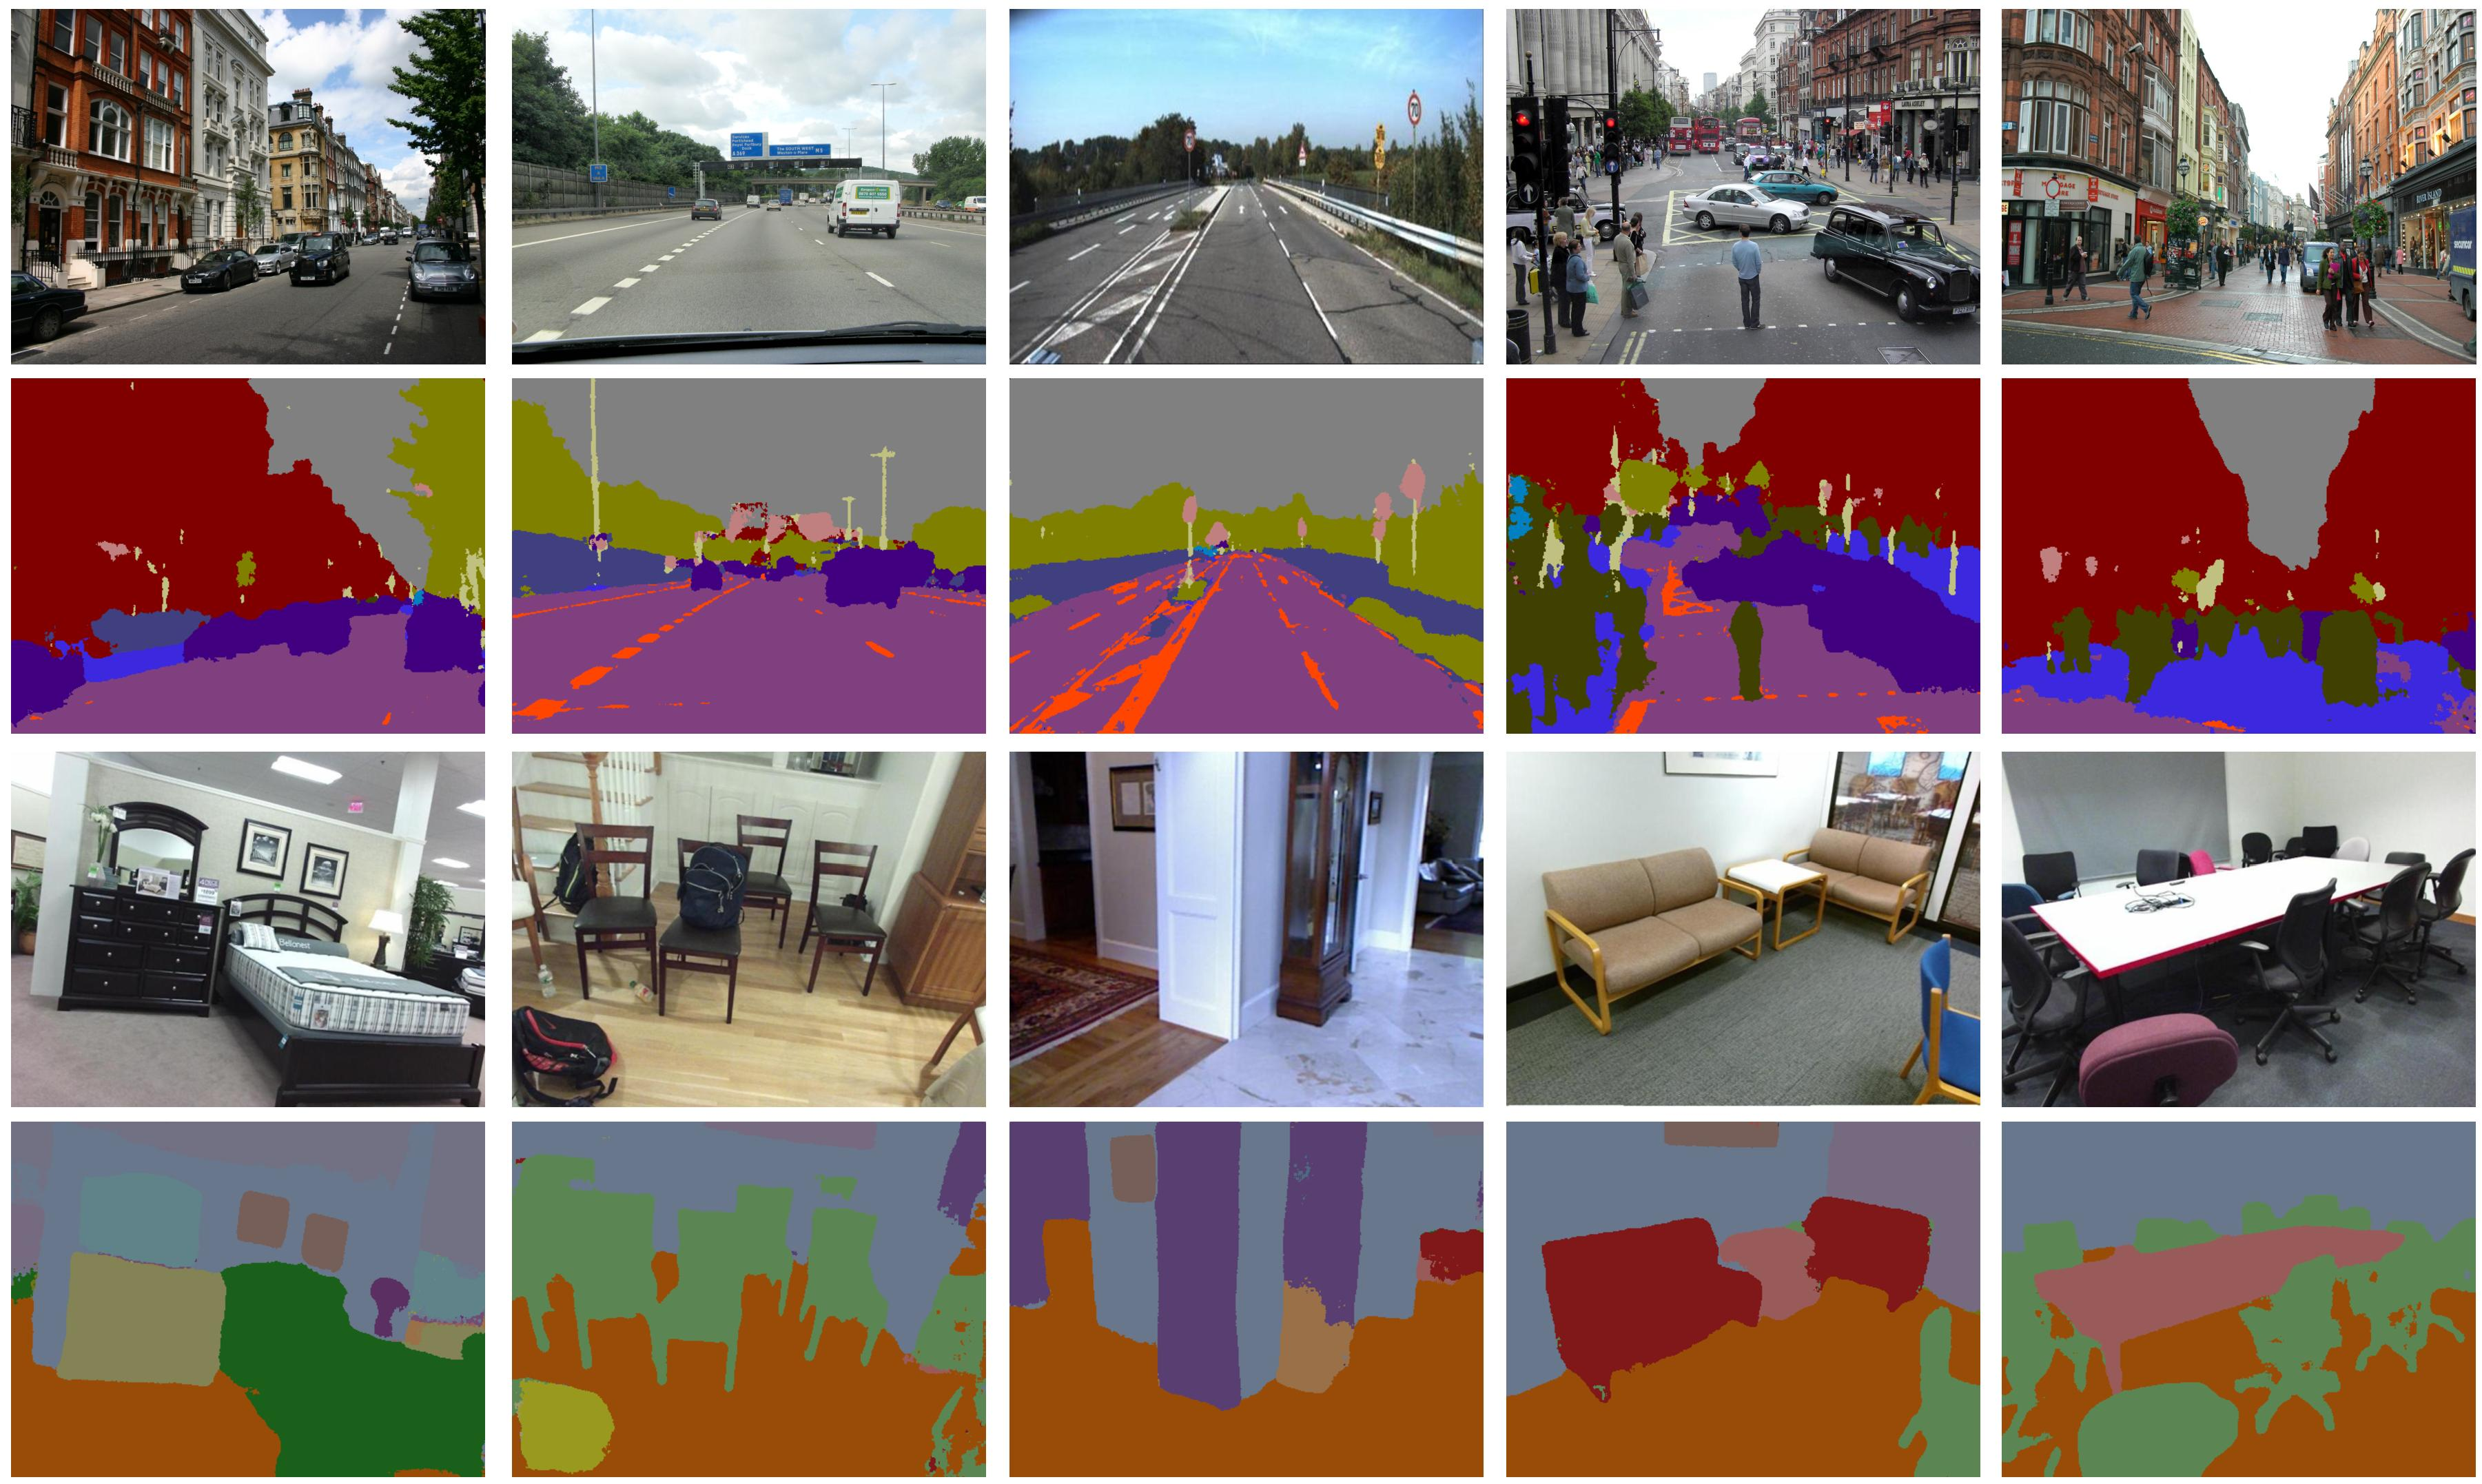
\includegraphics[width=\textwidth]{segnet/CamVidTeaserwithIndoorScenes.jpg}
\caption[SegNet semantic segmentation predictions on indoor and outdoor scenes.]{SegNet predictions on urban and highway scene test samples from the wild. To try our system yourself, please see our online web demo at \url{http://mi.eng.cam.ac.uk/projects/segnet/}.}
\label{Teaser}
\end{figure}

In this chapter, we address the problem of scene understanding. Scene understanding is a task which is fundamental to computer vision. It requires extracting information about what is where \citep{marr1982vision}. Visual scene understanding algorithms must extract information about objects and their contextual relationships from the observed environment. Scene understanding requires knowledge of semantics and geometry and can be broken down into many subtasks. In this work we focus on the tasks of semantic segmentation, instance segmentation and depth prediction. Collectively, these three representations provide a fine-grained, per-pixel representation of objects and their geometry.

We begin the chapter by proposing a deep convolutional encoder-decoder architecture, SegNet, capable of learning per-pixel output. Motivated by the problem of semantic segmentation, we analyse different architectures for upsampling features and producing dense pixel-wise output. We benchmark the efficacy of SegNet on many datasets on road scene, indoor and object segmentation datasets. Some results are shown in \cref{Teaser}.

For practical systems, it is important to understand what our models do not know. In \cref{seg_unc}, we discuss two types of uncertainty; aleatoric and epistemic uncertainty \citep{der2009aleatory}. We derive deep learning models which can capture both forms of uncertainty using Bayesian deep learning \citep{mackay1992practical} and probabilistic modelling. We build models for semantic segmentation and per-pixel depth estimation with these ideas. We show modelling uncertainty gives an improvement in performance. We empirically evaluate the quality of these uncertainty metrics and their properties with respect to novel examples, with increasing distinction from the training dataset.

However, scene understanding requires joint knowledge of semantics and geometry. In \cref{sec:mlttask}, we present a framework for designing models capable of learning many tasks from a single representation, using multi-task learning. We make the observation that the relative weighting of each task's loss greatly influences performance. We derive a loss function which learns the task weights using probabilistic modelling. The final model jointly predicts semantic segmentation, instance segmentation and depth regression. Interestingly, we show that jointly learning these tasks in a single multi-task model out-performs equivalent models individually trained on each task.

\section{Semantic Segmentation}
\label{segmentation}

We begin by introducing the task of semantic segmentation, which is a core task in scene understanding. Semantic pixel-wise segmentation requires an estimate of each pixel's semantic class (see \cref{Teaser}).
It is an active topic of research, fuelled by challenging datasets \citep{brostow2009semantic,silberman2012indoor,Geiger2012CVPR,pascal,song2015sun,Cordts2016Cityscapes}. Before the arrival of deep learning, the best performing methods mostly relied on hand engineered features classifying pixels independently. Typically, an image patch was fed into a classifier, \textit{e.g.} random forests \citep{Jamie2,brostow2008segmentation} or boosting \citep{Sturgess,LadickyECCV}, to predict the class probabilities of the centre pixel. Features based on appearance \citep{Jamie2} or motion and appearance \citep{brostow2008segmentation,Sturgess, LadickyECCV} have been explored. These per-pixel noisy predictions (often called \textit{unary} terms) from the classifiers are then smoothed by using a pair-wise (or higher order) conditional random fields (CRFs) \citep{Sturgess,LadickyECCV} to improve the accuracy. More recent approaches have aimed to produce high quality unaries by trying to predict the labels for all the pixels in a patch as opposed to only the centre pixel. This improves the results of random forest based unaries \citep{kontschieder2011structured}, but reduces performance on thin structures. Dense depth maps have also been used as input for classification using Random Forests \citep{zhang2010semantic}. Another approach argues for the use of a combination of popular hand designed features and spatio temporal super-pixels to obtain higher accuracy \citep{tighe2013superparsing}.

Indoor RGB-D pixel-wise semantic segmentation has also gained popularity since the release of the NYU dataset \citep{silberman2012indoor} which contains labelled RGB-D data collected from a Kinect sensor. Many papers demonstrate that inputting depth modality significantly improves segmentation performance \citep{ren2012rgb,silberman2012indoor,Hermans14ICRA,gupta2013perceptual}. However, all these methods use hand-engineered features for classifying RGB-D images. 

The success of deep convolutional neural networks for object classification has more recently led to researchers to exploit their feature learning capabilities for structured prediction problems such as segmentation. There have also been attempts to apply networks designed for object categorization to segmentation, particularly by replicating the deepest layer features in blocks to match image dimensions \citep{FarabetPAMI,FarabetPurityCover,Grangier,Gatta}. However, the resulting classification is coarse \citep{Grangier}. Another approach using recurrent neural networks \citep{pinheiro2014recurrent} merges several low resolution predictions to create input image resolution predictions. These techniques are already an improvement over hand engineered features \citep{FarabetPAMI} but their ability to delineate boundaries is poor. 

Newer deep architectures \citep{long2015fully,NohDeconvNets,eigen2015predicting,DecoupledNet,CRFRNN} particularly designed for segmentation have advanced the state-of-the-art by learning to decode or map low resolution image representations to pixel-wise predictions. These methods rely on pre-trained features from the large ImageNet object classification dataset \citep{deng2009imagenet}. For example, Fully Convolutional Networks (FCN) \citep{long2015fully} learns to up-sample its input feature map(s) and combines them with the corresponding encoder feature map to produce a dense output. It has a large number of trainable parameters in the encoder network (134M) but a very small decoder network (0.5M). The overall large size of this network makes it hard to train end-to-end on a relevant task. Therefore, the authors use a stage-wise training process. Each decoder in the decoder network is progressively added to an existing trained network. The network is grown until no further increase in performance is observed. 

The approach in FCN forms the \textit{core segmentation engine} for a number of other approaches \citep{ParseNetRabinovich,UrtasunSegmentation,CRFRNN,chen2016deeplab}. These methods append CRFs as a post-processing method to clean the segmentation. These methods are slow as they require either MAP inference over a CRF \citep{lin2015efficient}, \citep{UrtasunSegmentation} or aids such as region proposals \citep{NohDeconvNets} for inference. We believe the perceived performance increase obtained by using a CRF is due to the lack of good decoding techniques in their core feed-forward segmentation engine. 

Multi-scale deep architectures are also being pursued \citep{eigen2015predicting,lin2015efficient,hariharan2015hypercolumns,ParseNetRabinovich}. The common idea is to use features extracted at multiple scales to provide both local and global context \citep{mostajabi2014feedforward} and the using feature maps of the early encoding layers retain more high frequency detail leading to sharper class boundaries. Some of these architectures are difficult to train due to their large parameter size \citep{eigen2015predicting}. Again, a multi-stage training process is employed along with data augmentation. Inference is also expensive with multiple convolutional pathways for feature extraction.

All of the latest state-of-the-art semantic segmentation models use supervised deep learning \citep{badrinarayanan2017segnet,long2015fully}, benefiting from residual architectures \citep{he2016deep,huang2017densely}. Recent work has focused on improving the receptive field of features and providing them with more context for semantic reasoning, for example using dilated convolutions \citep{YuKoltun2016} and pyramid spatial pooling \citep{zhao2017pspnet}. We have also seen semantic segmentation combined with other tasks, such as instance segmentation \citep{he2017maskrcnn} and geometry \citep{kendall2017multi} in multi-task learning settings.

In the next section, we introduce the SegNet architecture, which was one of the first end-to-end deep convolutional neural networks for semantic segmentation. We compare the different decoding techniques to form pixel-wise prediction with deep learning and benchmark our approach on a number of challenging datasets.

\section{SegNet Architecture}
\label{segnet}

\begin{figure*}[t]
\center
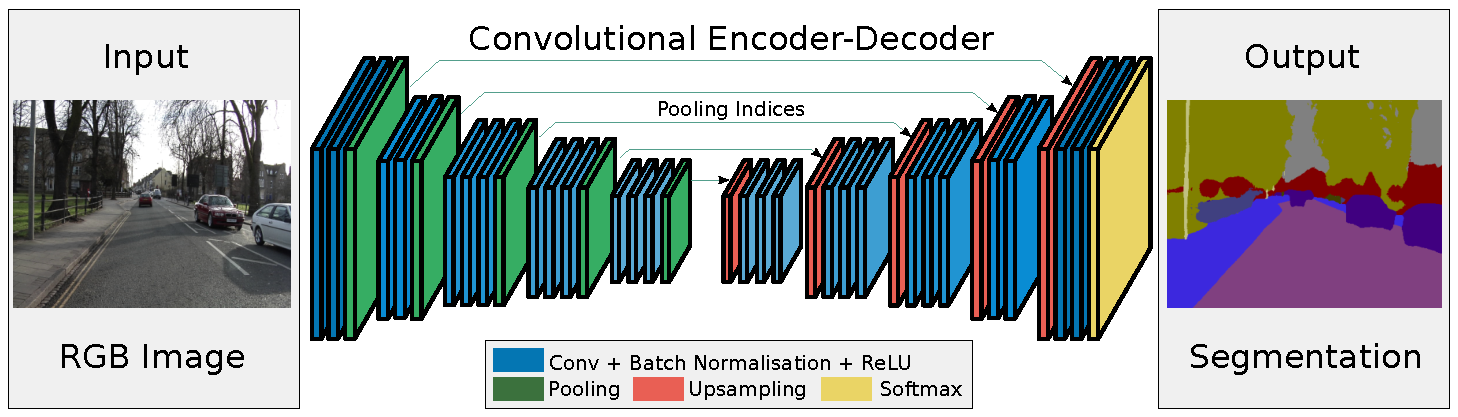
\includegraphics[width=0.95\textwidth]{segnet/segnet_softmax.pdf}
\caption[SegNet architecture.]{An illustration of the SegNet architecture. There are no fully connected layers and hence it is only convolutional. The decoder upsamples the encoded features using the corresponding pooling indices from the encoder to produce sparse feature maps. It then performs convolution with a trainable filter bank to densify the feature map. The final decoder output feature maps are fed to a softmax classifier for pixel-wise classification.}
\label{SegNetArchitecture}
\end{figure*}

The latest semantic segmentation architectures have tried to directly adopt deep architectures designed for category prediction to pixel-wise labelling \citep{long2015fully,FarabetPAMI}. The results, although very encouraging, appear coarse \citep{chen2016deeplab}. This is primarily because max-pooling and sub-sampling reduce feature map resolution in the encoder for recognition tasks. In this section, we design SegNet, a deep convolutional encoder-decoder architecture capable of outputting pixel-wise labels at full resolution. Our motivation to design SegNet arises from this need to map low resolution features to input resolution for pixel-wise classification. This mapping must produce features which are useful for accurate boundary localization. 

Our architecture, SegNet, is designed to be a \textit{core segmentation engine} for pixel-wise semantic segmentation. It is primarily motivated by road scene understanding applications which require the ability to model appearance (road, building), shape (cars, pedestrians) and understand the spatial-relationship (context) between different classes such as road and side-walk. In typical road scenes, the majority of the pixels belong to large classes such as road, building or sky and hence the network must produce smooth segmentations. The engine must also have the ability to delineate moving and other objects based on their shape despite their small size. Hence it is important to retain boundary information in the extracted image representation. From a computational perspective, it is necessary for the network to be efficient in terms of both memory and computation time during inference. It must also be able to train end-to-end in order to jointly optimise all the weights in the network using an efficient weight update technique such as stochastic gradient descent (SGD) \citep{Bottou}. Networks that are trained end-to-end or equivalently those that do not use multi-stage training \citep{long2015fully} or other supporting aids such as region proposals \citep{NohDeconvNets} help establish benchmarks that are more easily repeatable. The design of SegNet arose from a need to match these criteria.

SegNet has an encoder network and a corresponding decoder network, followed by a final pixel-wise classification layer. This architecture is illustrated in \cref{SegNetArchitecture}. The encoder network consists of $13$ convolutional layers which is topologically identical to the convolutional layers in VGG16 \citep{simonyan2014very}. We can therefore initialize the training process from weights trained for classification on large datasets \citep{deng2009imagenet}. We remove the fully connected layers of VGG16 which makes the SegNet encoder network significantly smaller (from $134$ million parameters to $14.7$ million) than many other recent architectures \citep{long2015fully,NohDeconvNets,ParseNetRabinovich,DecoupledNet}. 

The key component of SegNet is the decoder network which consists of a hierarchy of decoders one corresponding to each encoder. Of these, the appropriate decoders use the max-pooling indices received from the corresponding encoder to perform non-linear upsampling of their input feature maps. This idea was inspired from an architecture designed for unsupervised feature learning \citep{Ranzato}. Reusing max-pooling indices in the decoding process has several practical advantages; (i) it improves boundary delineation, (ii) it reduces the number of  parameters enabling end-to-end training, and (iii) this form of upsampling can be incorporated into any encoder-decoder architecture such as \citep{long2015fully,CRFRNN} with slight modification. The final decoder output is fed to a multi-class softmax classifier to produce class probabilities for each pixel independently.

Each \textit{encoder} in the encoder network performs convolution with a filter bank to produce a set of feature maps. These are then batch normalized \citep{BN}). Then an element-wise rectified-linear non-linearity (ReLU) $max(0,x)$ is applied. Following that, max-pooling with a $2\times2$ window and stride $2$ (non-overlapping window) is performed and the resulting output is sub-sampled by a factor of $2$. Max-pooling is used to achieve translation invariance over small spatial shifts in the input image. Sub-sampling results in a large receptive field for each pixel in the feature map. However, sub-sampling reduces spatial resolution of the features which is not beneficial for segmentation where boundary delineation is vital. Therefore, it is necessary to \textit{capture and store} boundary information in the encoder feature maps before sub-sampling is performed. If memory during inference is not constrained, then all the encoder feature maps (after sub-sampling) can be stored. This is usually not the case in practical applications and hence we propose a more efficient way to store this information. It involves storing only the max-pooling \textit{indices}, i.e, the locations of the maximum feature value in each pooling window is memorized for each encoder feature map. In principle, this can be done using 2 bits for each $2\times2$ pooling window and is thus much more efficient to store as compared to memorizing feature map(s) in float precision (such as U-Net \citep{ronneberger2015u}). As we show later in this work, this lower memory storage results in a slight loss of accuracy but is still suitable for practical applications.

The appropriate \textit{decoder} in the decoder network upsamples its input feature map(s) using the memorized max-pooling indices from the corresponding encoder feature map(s). This step produces sparse feature map(s). This SegNet decoding technique is illustrated in \cref{Upsampling}. These feature maps are then convolved with a trainable decoder filter bank to produce dense feature maps. A batch normalization step is then applied to each of these maps. Note that the decoder corresponding to the first encoder (closest to the input image) produces a multi-channel feature map, although its encoder input has 3 channels (RGB). This is unlike the other decoders in the network which produce feature maps with the same number of size and channels as their encoder inputs. The high dimensional feature representation at the output of the final decoder is fed to a trainable soft-max classifier. This soft-max classifies each pixel independently. The output of the soft-max classifier is a K channel image of probabilities where K is the number of classes. The predicted segmentation corresponds to the class with maximum probability at each pixel.

In the following Sections, we evaluate the performance of SegNet on a number of datasets \citep{pascal,hariharan2011semantic} and scene understanding challenges such as CamVid road scene segmentation \citep{brostow2009semantic}. We analyse different decoding techniques and the practical trade-offs when designing segmentation architecture. In addition, we present a real-time online demo of road scene segmentation into 11 classes of interest for autonomous driving (see \cref{Teaser}). Some example test results produced on randomly sampled road scene images from the internet are shown in \cref{Teaser}.

\begin{figure*}
\centering
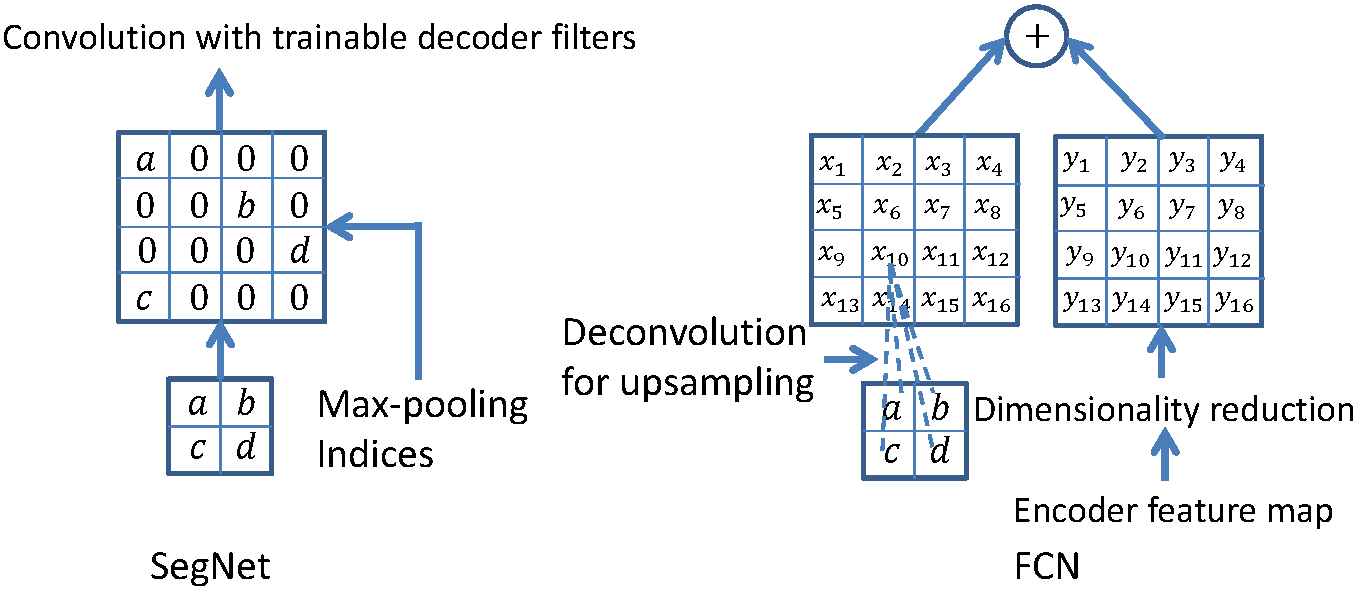
\includegraphics[width=\textwidth]{segnet/decoderVariantsNew.pdf}
\caption[SegNet decoder.]{An illustration of SegNet and FCN \citep{long2015fully} decoders. $a,b,c,d$ correspond to values in a feature map. SegNet uses the max pooling indices to upsample (without learning) the feature map(s) and convolves with a trainable decoder filter bank. FCN upsamples by learning to deconvolve the input feature map and adds the corresponding encoder feature map to produce the decoder output. This feature map is the output of the max-pooling layer (includes sub-sampling) in the corresponding encoder. Note that there are no trainable decoder filters in FCN.}
\label{Upsampling}
\end{figure*}

\subsection{Decoder Variants}
\label{Variants}

One of the main contributions of this Section is our analysis of decoding techniques for semantic segmentation. Most recent deep architectures for segmentation have identical encoder networks, \textit{i.e.} VGG16 \citep{simonyan2014very} or ResNet101 \citep{he2016deep}, but differ in the form of the decoder network, training and inference. Another common feature is they have trainable parameters in the order of hundreds of millions and thus encounter difficulties in performing end-to-end training \citep{NohDeconvNets}. The difficulty of training these networks has led to multi-stage training \citep{long2015fully}, appending networks to a pre-trained core segmentation engine such as FCN \citep{CRFRNN}, use of supporting aids such as region proposals for inference \citep{NohDeconvNets}, disjoint training of classification and segmentation networks \citep{DecoupledNet} and use of additional training data for pre-training \citep{ParseNetRabinovich} \citep{mottaghi2014role} or for full training \citep{CRFRNN}. In addition, performance boosting post-processing techniques \citep{chen2016deeplab} have also been popular. Although all these factors improve performance on challenging benchmarks \citep{pascal}, it is unfortunately difficult from their quantitative results to disentangle the key design factors necessary to achieve good performance. We therefore analyse many segmentation decoders in a controlled setting.

In order to analyse SegNet and compare its performance with other decoder variants we use a smaller version of SegNet, termed \textbf{SegNet-Basic}, which has 4 encoders and 4 decoders. All the encoders in SegNet-Basic perform max-pooling and sub-sampling and the corresponding decoders upsample its input using the received max-pooling indices. Batch normalization is used after each convolutional layer in both the encoder and decoder network. No biases are used after convolutions and no ReLU non-linearity is present in the decoder network. Further, a constant kernel size of $7\times7$ over all the encoder and decoder layers is chosen to provide a wide context for smooth labelling \textit{i.e.} a pixel in the deepest layer feature map (layer $4$) can be traced back to a context window in the input image of $106\times106$ pixels. This small size of SegNet-Basic allows us to explore many different variants (decoders) and train them in reasonable time. Similarly we create \textbf{FCN-Basic}, a comparable version of FCN for our analysis which shares the same encoder network as SegNet-Basic but with the FCN decoding technique in the corresponding decoders.  

On the left in \cref{Upsampling} is the decoding technique used by SegNet (also SegNet-Basic), where there is no learning involved in the upsampling step. However, the upsampled maps are convolved with trainable multi-channel decoder filters to densify the sparse inputs. Each decoder filter has the same number of channels as the number of upsampled feature maps. A smaller variant is one where the decoder filters are single channel, i.e they only convolve their corresponding upsampled feature map. This variant (\textbf{SegNet-Basic-SingleChannelDecoder}) reduces the number of trainable parameters and inference time significantly.

On the right in \cref{Upsampling} is the FCN (also FCN-Basic) decoding technique \citep{long2015fully}. The important design element of the FCN model is dimensionality reduction step of the encoder feature maps. This \textit{compresses} the encoder feature maps which are then used in the corresponding decoders. Dimensionality reduction of the encoder feature maps, say of 64 channels, is performed by convolving them with $1\times 1\times 64\times K$ trainable filters, where $K$ is the number of classes. The compressed $K$ channel final encoder layer feature maps are the input to the decoder network. In a decoder of this network, upsampling is performed by convolution using a trainable \textit{multi-channel upsampling kernel}. We set the kernel size to $8\times8$. This manner of upsampling is also termed as \textit{sub-pixel convolution}, \textit{deconvolution} or \textit{transposed convolution}. Note that in SegNet the multi-channel convolution using trainable decoder filters is performed after upsampling to densifying feature maps. The upsampled feature map in FCN is then added to the corresponding resolution encoder feature map to produce the output decoder feature map. The upsampling kernels are initialized using bilinear interpolation weights \citep{long2015fully}. 

The FCN decoder model requires storing encoder feature maps during inference. This can be memory intensive, for e.g. storing 64 feature maps of the first layer of FCN-Basic at $180\times240$ resolution in 32 bit floating point precision takes 11MB. This can be made smaller using dimensionality reduction to the 11 feature maps which requires $\approx$ 1.9MB storage. SegNet on the other hand requires almost negligible storage cost for the pooling indices ($0.17$MB if stored using 2 bits per $2\times2$ pooling window). We can also create a variant of the FCN-Basic model which discards the encoder feature map addition step and only learns the upsampling kernels (\textbf{FCN-Basic-NoAddition}). 

In addition to the above variants, we study upsampling using fixed bilinear interpolation weights which therefore requires no learning for upsampling (\textbf{Bilinear-Interpolation}). At the other extreme, we can add 64 encoder feature maps at each layer to the corresponding output feature maps from the SegNet decoder to create a more memory intensive variant of SegNet (\textbf{SegNet-Basic-EncoderAddition}). Another and more memory intensive FCN-Basic variant (\textbf{FCN-Basic-NoDimReduction}) is where there is no dimensionality reduction performed for the encoder feature maps. Finally, please note that to encourage reproduction of our results we release the Caffe \citep{jia2014caffe} implementation of all the variants\footnote{See \url{http://mi.eng.cam.ac.uk/projects/segnet/} for our SegNet code and web demo.}. 

We also tried other generic variants where feature maps are simply upsampled by \textit{replication} \citep{FarabetPAMI}, or by using a fixed (and sparse) array of indices for upsampling. These performed quite poorly in comparison to the above variants. A variant without max-pooling and sub-sampling in the encoder network (decoders are redundant) consumes more memory, takes longer to converge and performs poorly. 

\subsection{Training}
\label{Training}


\afterpage{%
    \clearpage% Flush earlier floats (otherwise order might not be correct)
    \begin{landscape}% Landscape page
\begin{table*}[t]
\centering
\resizebox{\linewidth}{!}{
\begin{tabular}{c|c|c|c|ccc|ccc}
%\hline
\multicolumn{4}{c}{} &  \multicolumn{3}{c}{Median frequency balancing} & \multicolumn{3}{|c}{Natural frequency balancing} \\
\hline
& & Encoder & Infer & \multicolumn{3}{c|}{} &  \multicolumn{3}{c}{}\\
Variant &Params (M) &  storage (MB) &  time (ms) & G & C & IoU & G & C & IoU \\ \hline \hline
\multicolumn{10}{c}{Fixed upsampling} \\ \hline
Bilinear-Interpolation & 0.625 & 0 & 24.2 & 77.9 & 61.1 & 43.3 & 82.7 & 52.5 & 43.8 \\ \hline
\multicolumn{10}{c}{Upsampling using max-pooling indices} \\ \hline
SegNet-Basic & 1.425 & 1x & 52.6 & 82.7 & 62.0 & 47.7 & 84.0 & 54.6 & 46.3 \\ \hline
SegNet-Basic-EncoderAddition &1.425 & 64x & 53.0 & 83.4 & \textbf{63.6} & 48.5 & \textbf{84.2} & 56.5 & \textbf{47.7} \\ \hline
SegNet-Basic-SingleChannelDecoder& 0.625 &  1x & 33.1 &  81.2 & 60.7 & 46.1 & 83.5 & 53.9 & 45.2 \\ \hline
\multicolumn{10}{c}{Learning to upsample (bilinear initialisation)} \\ \hline
FCN-Basic & 0.65 & 11x & 24.2  & 81.7 & 62.4 & 47.3 &  83.9 & 55.6 & 45.0 \\ \hline
FCN-Basic-NoAddition &0.65 & n/a & 23.8 & 80.5 & 58.6 & 44.1 & 82.3 & 53.9 & 44.2 \\ \hline
FCN-Basic-NoDimReduction &1.625 & 64x & 44.8 & \textbf{84.1} & 63.4 & \textbf{50.1} & 83.5 & \textbf{57.3} & 47.0 
\\ \hline
FCN-Basic-NoAddition-NoDimReduction &1.625 & 0 & 43.9 & 80.5 & 61.6 & 45.9 & 83.7 & 54.8 & 45.5 \\ \hline 
\end{tabular}}

\caption[Quantitative segmentation decoder comparison.]{Comparison of decoder variants. We quantify the performance using global (G), class average (C) and mean of intersection over union (IoU) metrics. The testing accuracies are shown as percentages for both natural frequency and median frequency balanced training loss function. SegNet-Basic performs at the same level as FCN-Basic but requires only storing max-pooling indices and is therefore more memory efficient during inference. Note that the theoretical memory requirement reported is based only on the size of the first layer encoder feature map. Networks with larger decoders and those using the encoder feature maps in full perform best, although they are least efficient.}
\label{PoolingQuantCAFFE}
\end{table*}
\end{landscape}}

We use the CamVid road scenes dataset to benchmark the performance of the decoder variants. This dataset is small, consisting of 367 training and 233 testing RGB images (day and dusk scenes) at $360\times480$ resolution. The challenge is to segment $11$ classes such as road, building, cars, pedestrians, signs, poles, side-walk \textit{etc}. We perform local contrast normalization \citep{Jarrett} to the RGB input.

The encoder and decoder weights were all initialized using the technique described in He \emph{et~al.} \citep{he2015delving}. To train all the variants we use stochastic gradient descent (SGD) with a fixed learning rate of 0.1 and momentum of 0.9 \citep{Bottou} using our Caffe implementation of SegNet-Basic \citep{jia2014caffe}. We train the variants until the training loss converges. Before each epoch, the training set is shuffled and each mini-batch (12 images) is then picked in order thus ensuring that each image is used only once in an epoch. We select the model which performs highest on a validation dataset.

We use the cross-entropy loss \citep{long2015fully} as the objective function for training the network. The loss is averaged up over all the pixels in a mini-batch which contain a valid label. When there is large variation in the number of pixels in each class in the training set (e.g road, sky and building pixels dominate the CamVid dataset) then there is a need to weight the loss differently based on the true class. This is termed \textit{class balancing}. We use \textit{median frequency balancing} \citep{eigen2015predicting} where the weight assigned to a class in the loss function is the ratio of the median of class frequencies computed on the entire training set divided by the class frequency. This implies that larger classes in the training set have a weight smaller than $1$ and the weights of the smallest classes are the highest. We also experimented with training the different variants without class balancing or equivalently using \textit{natural frequency balancing}.

\subsection{Analysis}
\label{Analysis}
To compare the quantitative performance of the different decoder variants, we use three commonly used performance measures: global accuracy (G) which measures the percentage of pixels correctly classified in the dataset, class average accuracy (C) is the mean of the predictive accuracy over all classes and mean intersection over union (IoU) over all classes as used in the Pascal VOC12 challenge \citep{pascal}. The mean IoU metric is the hardest metric since it penalizes false positive predictions unlike class average accuracy. However, IoU metric is not optimized for directly through the class balanced cross-entropy loss. 

We test each variant after each $1000$ iterations of optimization on the CamVid validation set until the training loss converges. With a training mini-batch size of 12 this corresponds to testing approximately every 33 epochs (passes) through the training set. We select the iteration wherein the global accuracy is highest amongst the evaluations on the validation set. We report all the three measures of performance at this point on the held-out CamVid test set. Although we use class balancing while training the variants, it is still important to achieve high global accuracy to result in an overall smooth segmentation. Another reason is that the contribution of segmentation towards autonomous driving is mainly for delineating classes such as roads, buildings, side-walk, sky. These classes dominate the majority of the pixels in an image and a high global accuracy corresponds to good segmentation of these important classes. We also observed that reporting the numerical performance when class average is highest can often correspond to low global accuracy indicating a perceptually noisy segmentation output.

In Table \ref{PoolingQuantCAFFE} we report the numerical results of our analysis. We also show the size of the trainable parameters and the highest resolution feature map or pooling indices storage memory, i.e, of the first layer feature maps after max-pooling and sub-sampling. We show the average time for one forward pass with our Caffe implementation, averaged over $50$ measurements using a $360\times480$ input on an NVIDIA Titan GPU with cuDNN v3 acceleration. We note that the upsampling layers in the SegNet variants are not optimised using cuDNN acceleration. We show the results for both testing and training for all the variants at the selected iteration. The results are also tabulated without class balancing (natural frequency) for training and testing accuracies. Below we analyse the results with class balancing.

From the Table \ref{PoolingQuantCAFFE}, we see that bilinear interpolation based upsampling without any learning performs the worst based on all the three measures of accuracy. All the other methods which either use learning for upsampling (FCN-Basic and variants) or learning decoder filters after upsampling (SegNet-Basic and its variants) perform significantly better. This emphasizes the need to learn decoders for segmentation. This is also supported by experimental evidence gathered by other authors when comparing FCN with SegNet-type decoding techniques \citep{NohDeconvNets}.

When we compare SegNet-Basic and FCN-Basic we see that both perform equally well on this test over all the three measures of accuracy. The difference is that SegNet uses less \textbf{memory} during inference since it only stores max-pooling indices. On the other hand FCN-Basic stores \textbf{encoder feature maps} in full which consumes much more memory (11 times more). SegNet-Basic has a decoder with 64 feature maps in each decoder layer. In comparison FCN-Basic, which uses dimensionality reduction, has fewer (11) feature maps in each decoder layer. This reduces the number of convolutions in the decoder network and hence FCN-Basic is faster during inference (forward pass). From another perspective, the decoder network in SegNet-Basic makes it overall a larger network than FCN-Basic. This endows it with more flexibility and hence achieves higher training accuracy than FCN-Basic for the same number of iterations. Overall we see that SegNet-Basic has an advantage over FCN-Basic when memory during inference is constrained but where inference time can be compromised to an extent. 

SegNet-Basic is most similar to FCN-Basic-NoAddition in terms of their decoders, although the decoder of SegNet is larger. Both learn to produce dense feature maps, either directly by learning to perform deconvolution as in FCN-Basic-NoAddition or by first upsampling and then convolving with trained decoder filters. 
The performance of SegNet-Basic is superior, in part due to its larger decoder size. Now, the accuracy of FCN-Basic-NoAddition is also lower as compared to FCN-Basic. This shows that it is important to capture the information present in the encoder feature maps for better performance. This can also explain the part of the reason why SegNet-Basic outperforms FCN-Basic-NoAddition. 

The size of the FCN-Basic-NoAddition-NoDimReduction model is slightly larger than SegNet-Basic and this makes it a fair comparison. The performance of this FCN variant is poorer than SegNet-Basic in test but also its training accuracy is lower for the same number of training epochs. This shows that using a larger decoder is not enough but it is also important to capture encoder feature map information to learn better. Here it is also interesting to see that SegNet-Basic has a competitive training accuracy when compared to larger models such FCN-Basic-NoDimReduction. 

Another interesting comparison between FCN-Basic-NoAddition and SegNet-Basic-SingleChannelDecoder shows that using max-pooling indices for upsampling and an overall larger decoder leads to better performance. This also lends evidence to SegNet being a good architecture for segmentation, particularly when there is a need to find a compromise between storage cos, accuracy versus inference time. In the best case, when both memory and inference time is not constrained, larger models such as FCN-Basic-NoDimReduction and SegNet-EncoderAddition are both more accurate than the other variants. Particularly, discarding dimensionality reduction in the FCN-Basic model leads to the best performance amongst the FCN-Basic variants. This once again emphasizes the trade-off involved between memory and accuracy in segmentation architectures.

The last column of Table \ref{PoolingQuantCAFFE} show the result when no class balancing is used (natural frequency). Here, we can observe that without weighting the results are poorer for all the variants, particularly for class average accuracy and mean IoU metric. The global accuracy is the highest without weighting since the majority of the scene is dominated by sky, road and building pixels. Apart from this all the inference from the comparative analysis of variants holds true for natural frequency balancing too. SegNet-Basic performs as well as FCN-Basic and is better than the larger FCN-Basic-NoAddition-NoDimReduction. The bigger but less efficient models FCN-Basic-NoDimReduction and SegNet-EncoderAddition perform better than the other variants.

We can now summarize the above analysis with the following general points.
\begin{enumerate}
\item The best performance is achieved when encoder feature maps are stored in full.
\item When memory during inference is constrained, then compressed forms of encoder feature maps (dimensionality reduction, max-pooling indices) can be stored and used with an appropriate decoder (e.g. SegNet type) to improve performance.
\item Larger decoders increase performance for a given encoder network.
\end{enumerate}



\subsection{Benchmarking}
\label{Benchmarking}
We quantify the performance of SegNet on three different benchmarks using our Caffe implementation \footnote{Our web demo and Caffe implementation is available for evaluation at \url{http://mi.eng.cam.ac.uk/projects/segnet/}}. Through this process we demonstrate the efficacy of SegNet for various scene segmentation tasks which have practical applications. In the first experiment, we test the performance of SegNet on the CamVid road scene dataset (see Sec. \ref{Training} for more information about this data). We use this result to compare SegNet with several methods including Random Forests \citep{Jamie2}, Boosting \citep{Jamie2,Sturgess} in combination with CRF based methods \citep{LadickyECCV}.  We also trained SegNet on a larger dataset of road scenes collected from various publicly available datasets \citep{brostow2009semantic,LabelMe,SpanishKITTI} and show that this leads to a large improvement in accuracy.

SUN RGB-D \citep{song2015sun} is a very challenging and large dataset of indoor scenes with $5285$ training and $5050$ testing images. The images are captured by different sensors and hence come in various resolutions. The task is to segment $37$ indoor scene classes including wall, floor, ceiling, table, chair, sofa etc. This task is made hard by the fact that object classes come in various shapes, sizes and in different poses. There are frequent partial occlusions since there are typically many different classes present in each of the test images. These factors make this one of the hardest segmentation challenges. We only use the RGB modality for our training and testing. Using the depth modality would necessitate architectural modifications/redesign \citep{long2015fully}. Also the quality of depth images from current cameras require careful post-processing to fill-in missing measurements. They may also require using fusion of many frames to robustly extract features for segmentation.

Pascal VOC12 \citep{pascal} is a RGB dataset for segmentation with $12031$ combined training and validation images of indoor and outdoor scenes. The task is to segment $21$ classes such as bus, horse, cat, dog, boat from a varied and large background class. The foreground classes often occupy a small part of an image. The evaluation is performed remotely on $1456$ images.

In all three benchmark experiments, we select random $224\times224$ resolution crops from the images for training. We used SGD with momentum to train SegNet. The learning rate was fixed to 0.001 and momentum to 0.9. The mini-batch size was 4. The optimization was performed for 100 epochs and then tested.

\begin{figure*}
\centering
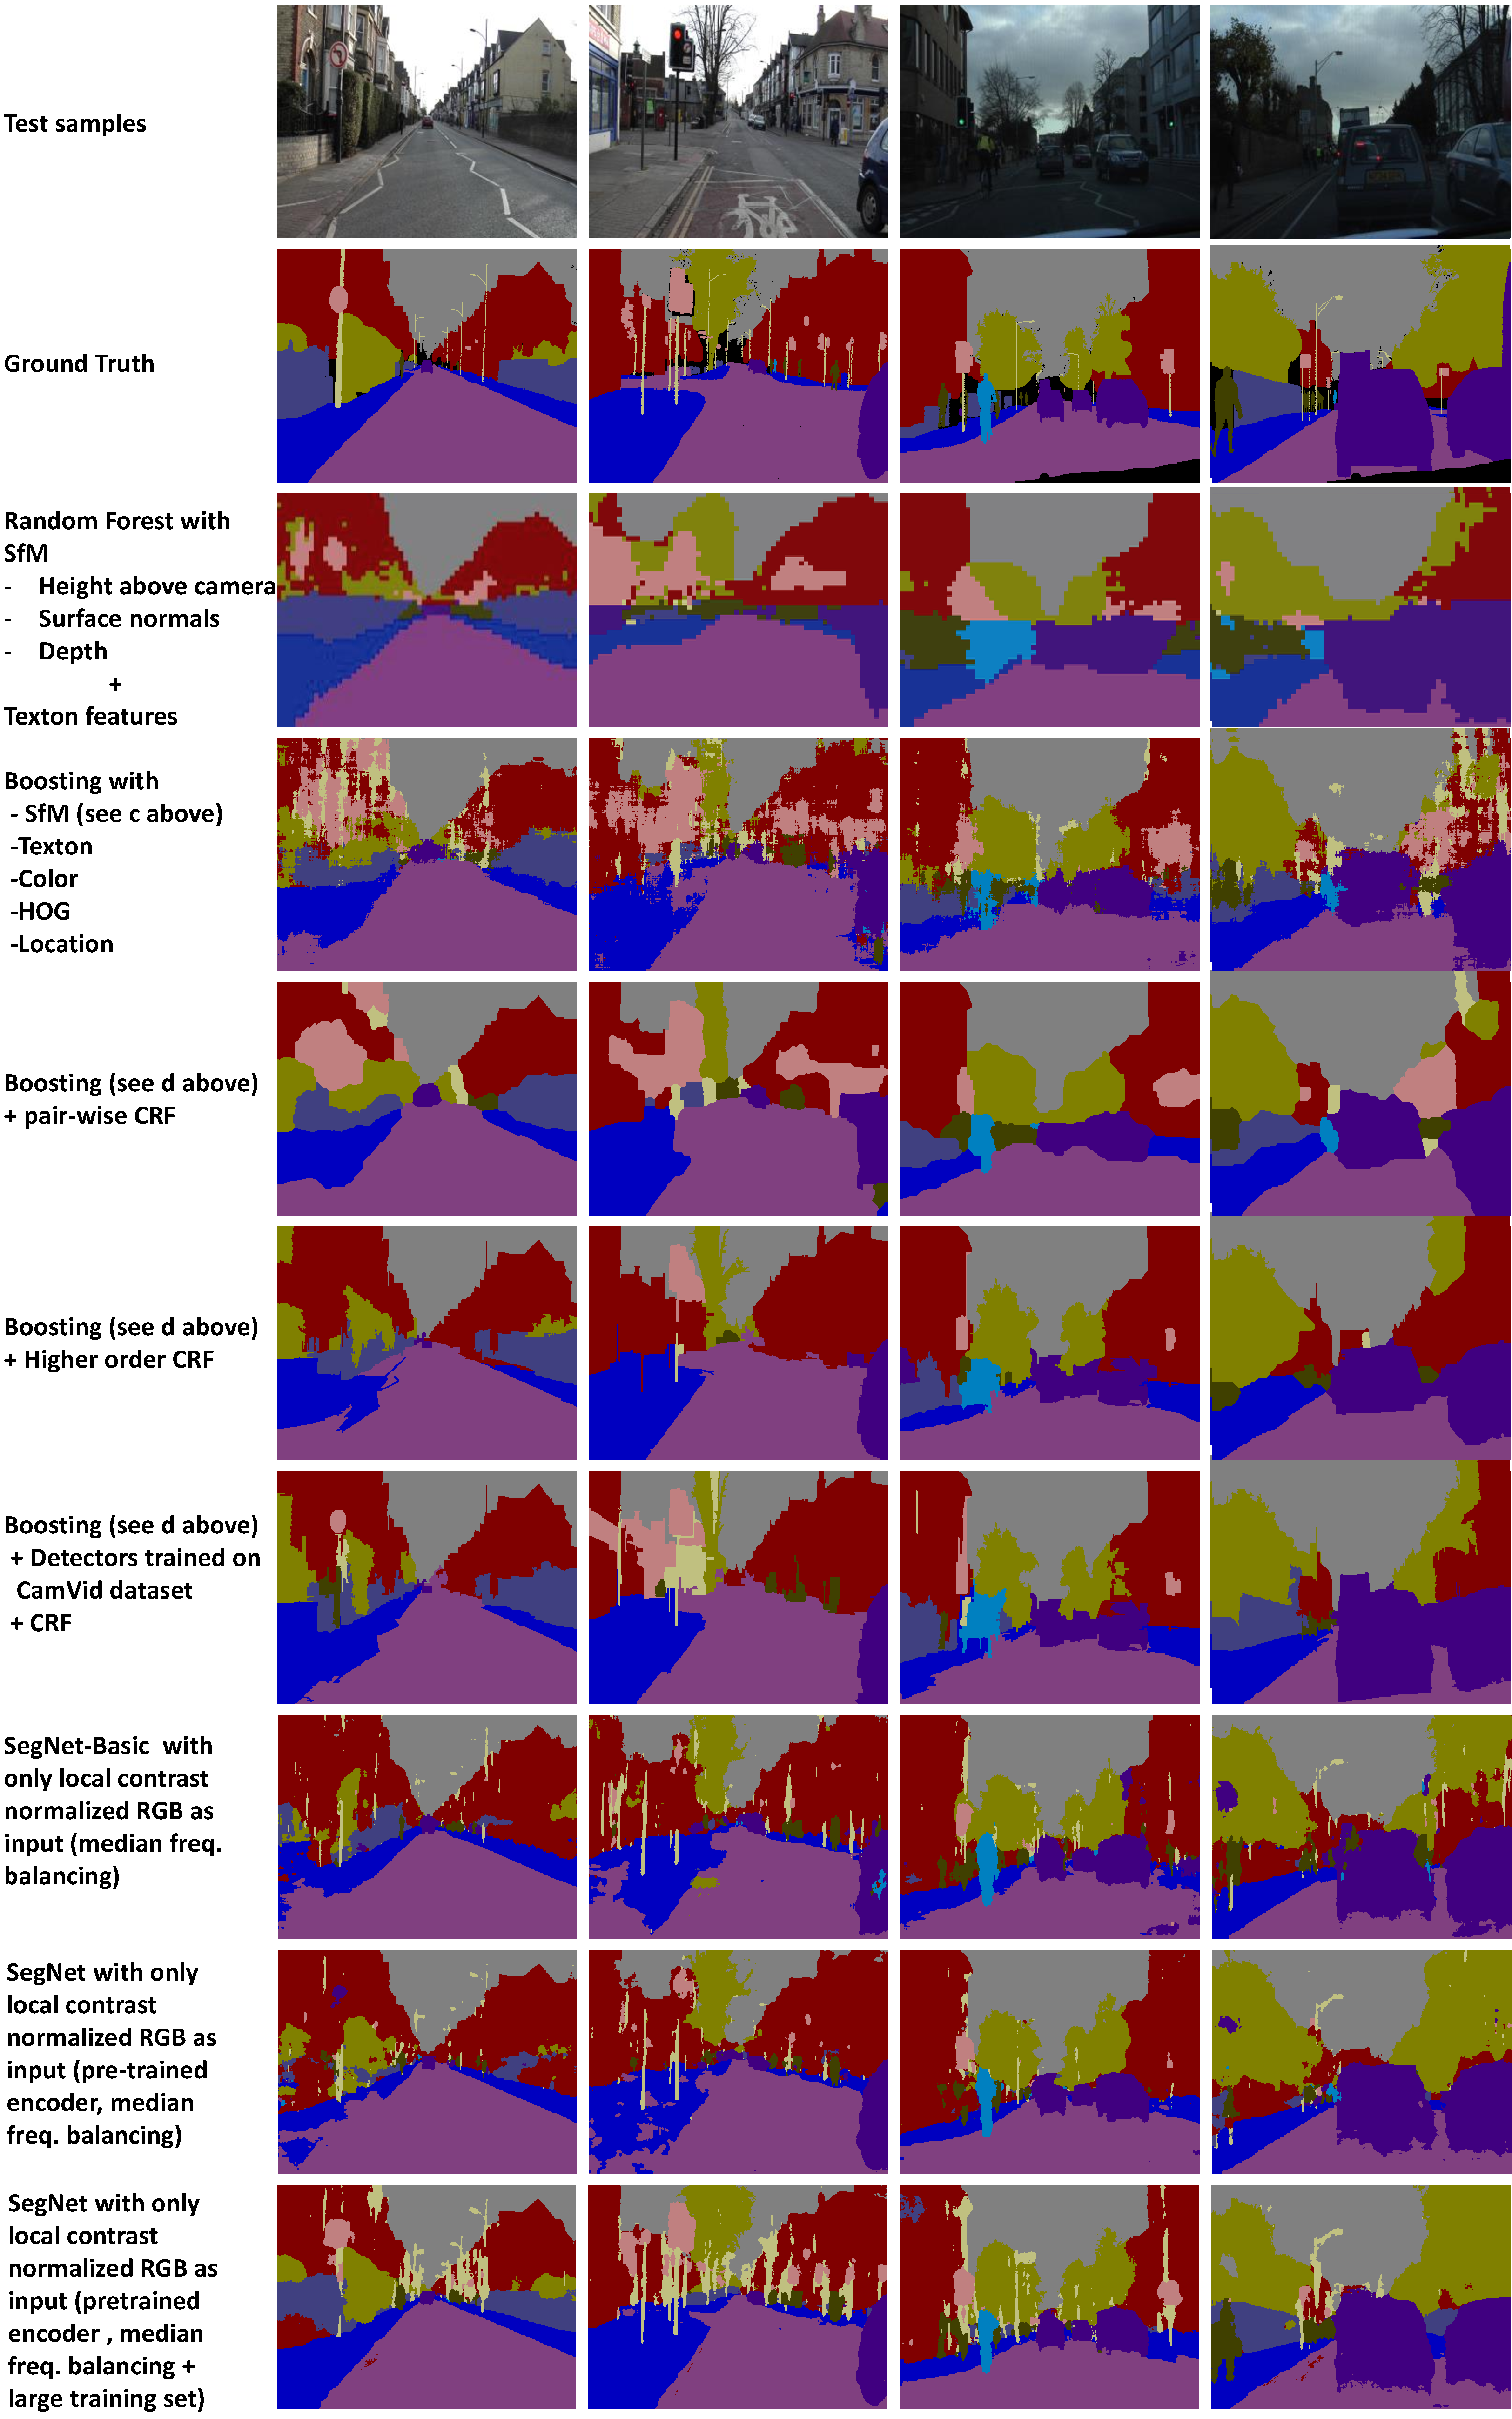
\includegraphics[width=0.85\textwidth]{segnet/CamVidQualitative.pdf}
\caption[CamVid qualitative results.]{Results on CamVid day and dusk test samples. The evolution of results from various patch based predictions \citep{Jamie2,brostow2008segmentation}, then CRF smoothing models \citep{LadickyECCV,Sturgess} and finally SegNet.
}
\label{CamVidQualy}
\end{figure*}

\subsubsection{CamVid Road Scenes}
\label{CamVid}
A number of outdoor scene datasets are available for semantic parsing \citep{gould2009decomposing,russell2008labelme,brostow2009semantic,Geiger2012CVPR}. From these, we choose to benchmark SegNet using the CamVid dataset \citep{brostow2009semantic} because it contains video sequences. This enables us to compare our proposed architecture with those which use motion and structure \citep{LadickyECCV,Sturgess,brostow2008segmentation} and video segments \citep{tighe2013superparsing}. We also combine \citep{gould2009decomposing,russell2008labelme,brostow2009semantic,Geiger2012CVPR} to form an ensemble of 3433 images to train SegNet for an additional benchmark.

The qualitative comparisons of SegNet-Basic and SegNet predictions with several prominent algorithms (unaries, unaries+CRF) are shown in \cref{CamVidQualy} along with the input modalities used to train the methods. The qualitative results show the ability of the proposed architectures to segment small (cars, pedestrians, bicyclist) classes while producing a smooth segmentation of the overall scene. The unary-only methods (like Random Forests or Boosting) which are trained to predict the label of the centre-pixel of a small patch produce low quality segmentations. Smoothing unaries with CRF's improve the segmentation quality considerably with higher order CRF's performing best. Although the CRF based results appear smooth, upon close scrutiny, we see that shape segmentation of smaller but important classes such as bicyclists, pedestrians are poor. In addition, natural shapes of classes like trees are not preserved and the details like the wheels of cars are lost.  More dense CRF models \citep{koltun2011efficient} can be better but with additional cost of inference. SegNet-Basic and SegNet (without large dataset training) clearly indicate their ability to retain the natural shapes of classes such as bicyclists, cars, trees, poles etc better than CRF based approaches. The overall segmentation quality is also smooth except for the side-walk class. This is because the side-walk class is highly varied in terms of size and texture and this cannot be captured with a small training set. Another explanation could be that the size of the receptive fields of the deepest layer feature units are smaller than their theoretical estimates \citep{zhou2014object,ParseNetRabinovich} and hence unable to group all the side-walk  pixels into one class. Illumination variations also affect performance on cars in the dusk examples. However, several of these issues can be ameliorated by using larger amounts of training data. In particular, we see that smaller classes such as pedestrians, cars, bicyclists, column-pole are segmented better than other methods in terms of shape retention. The side-walk class is also segmented smoothly.


\afterpage{%
    \clearpage% Flush earlier floats (otherwise order might not be correct)
    \begin{landscape}% Landscape page
\begin{table*}[th]
 \resizebox{\linewidth}{!}{
\small{
\begin{tabular}{c|c|c|c|c|c|c|c|c|c|c|c|ccc}

\multicolumn{1}{c}{Method}                   & \multicolumn{1}{c}{\rotatebox{90}{Building}} & \multicolumn{1}{c}{\rotatebox{90}{Tree}} & \multicolumn{1}{c}{\rotatebox{90}{Sky}}  & \multicolumn{1}{c}{\rotatebox{90}{Car}}  & \multicolumn{1}{c}{\rotatebox{90}{Sign-Symbol}} & \multicolumn{1}{c}{\rotatebox{90}{Road}} & \multicolumn{1}{c}{\rotatebox{90}{Pedestrian}} & \multicolumn{1}{c}{\rotatebox{90}{Fence}} & \multicolumn{1}{c}{\rotatebox{90}{Column-Pole}} & \multicolumn{1}{c}{\rotatebox{90}{Side-walk}} & \multicolumn{1}{c}{\rotatebox{90}{Bicyclist}} & \multicolumn{1}{c}{\rotatebox{90}{Class avg.}} & \multicolumn{1}{c}{\rotatebox{90}{Global avg.}} & \multicolumn{1}{c}{\rotatebox{90}{Mean IoU}}\\ \hline \hline



SfM+Appearance  \citep{brostow2008segmentation}           & 46.2     & 61.9 & 89.7 & 68.6 & 42.9        & 89.5 & 53.6       & 46.6  & 0.7         & 60.5     & 22.5      & 53.0       & 69.1  & n/a      \\ \hline

Boosting    \citep{Sturgess}              & 61.9     & 67.3 & 91.1 & 71.1 & 58.5        & 92.9 & 49.5       & 37.6  & 25.8        & 77.8     & 24.7      & 59.8       & 76.4  & n/a      \\ \hline

Dense Depth Maps   \citep{zhang2010semantic}          & 85.3     & 57.3 & 95.4 & 69.2 & 46.5        & \textbf{98.5} & 23.8       & 44.3  & 22.0        & 38.1     & 28.7      & 55.4       & 82.1    & n/a    \\ \hline

Structured Random Forests \citep{kontschieder2011structured}& \multicolumn{11}{c|}{n/a}                                                                          & 51.4       & 72.5    & n/a    \\ \hline

Neural Decision Forests \citep{BuloNeural}  & \multicolumn{11}{c|}{n/a}                                                                          & 56.1       & 82.1   & n/a     \\ \hline

Local Label Descriptors  \citep{yang2012local}  & 80.7     & 61.5 & 88.8 & 16.4 & n/a         & 98.0 & 1.09       & 0.05  & 4.13        & 12.4     & 0.07      & 36.3       & 73.6    & n/a    \\ \hline

Super Parsing   \citep{tighe2013superparsing}           & 87.0     & 67.1 & 96.9 & 62.7 & 30.1        & 95.9 & 14.7       & 17.9  & 1.7         & 70.0     & 19.4      & 51.2       & 83.3    & n/a    \\ \hline
SegNet-Basic          &  81.3    & 72.0  & 93.0 & 81.3 & 14.8 & 93.3 & 62.4 & 31.5 & 36.3  & 73.7 & 42.6  &   62.0    & 82.7   &   47.7   \\ \hline
SegNet-Basic (layer-wise training \citep{SegNetarXiv})         & 75.0     & 84.6 & 91.2 & 82.7 & 36.9        & 93.3 & 55.0       & 37.5  & 44.8        & 74.1     & 16.0      & 62.9       & 84.3   & n/a     \\ \hline
SegNet    &  \textbf{88.8}   & 87.3 & 92.4  & 82.1 & 20.5 & 97.2 &  57.1 & 49.3  &  27.5       &  84.4   &  30.7     &   65.2    &  \textbf{88.5}  & 55.6     \\ \hline
SegNet (3.5K dataset training)   & 73.9  & \textbf{90.6}  & 90.1  & \textbf{86.4}  &  \textbf{69.8}  & 94.5 &   \textbf{86.8}   & \textbf{67.9}  &   \textbf{74.0}	   &  \textbf{94.7}	   &  \textbf{52.9}    & \textbf{80.1}  & 86.7 &       \textbf{60.4}\\ \hline

\multicolumn{15}{c}{CRF based approaches}                                                                                                       \\ \hline

Boosting + pairwise CRF  \citep{Sturgess} & 70.7     & 70.8 & 94.7 & 74.4 & 55.9        & 94.1 & 45.7       & 37.2  & 13.0        & 79.3     & 23.1      & 59.9       & 79.8  & n/a      \\ \hline

Boosting+Higher order \citep{Sturgess}    & 84.5     & 72.6 & \textbf{97.5} & 72.7 & 34.1        & 95.3 & 34.2       & 45.7  & 8.1         & 77.6     & 28.5      & 59.2       & 83.8    & n/a    \\ \hline

Boosting+Detectors+CRF \citep{LadickyECCV}   & 81.5     & 76.6 & 96.2 & 78.7 & 40.2        & 93.9 & 43.0       & 47.6  & 14.3        & 81.5     & 33.9      & 62.5       & 83.8    & n/a    \\ \hline
\end{tabular}
}}
\caption[CamVid quantitative results.]{Quantitative results on CamVid \citep{brostow2009semantic} consisting of 11 road scene categories. SegNet outperforms all the other methods, including those using depth, video and/or CRF's. In comparison with the CRF based methods SegNet predictions are more accurate in 8 out of the 11 classes. It also shows a good $\approx 15\%$ improvement in class average accuracy when trained on a large dataset of 3.5K images and this sets a new benchmark for the majority of the individual classes. Particularly noteworthy are the significant improvements in accuracy for the smaller/thinner classes. 
}
\label{CamVidQuant}
\end{table*}
\end{landscape}}

The quantitative results in Table \ref{CamVidQuant} show SegNet-Basic, SegNet obtain competitive results even without CRF based processing. This shows the ability of the deep architecture to extract meaningful features from the input image and map it to accurate and smooth class segment labels. SegNet is better in performance than SegNet-Basic although trained with the same (small) training set. This indicates the importance of using pre-trained encoder weights and a deeper architecture. Interestingly, the use of the bigger and deeper SegNet architecture improves the accuracy of the larger classes as compared to SegNet-Basic and not the smaller classes as one might expect. We also find that SegNet-Basic \citep{SegNetarXiv} trained in a layer-wise manner using L-BFGS \citep{Nocedal} also performs competitively and is better than SegNet-Basic trained with SGD (see Sec. \ref{Training}). This is an interesting training approach but needs further research in order for it scale to larger datasets.

The most interesting result is the approximately $15\%$ performance improvement in class average accuracy that is obtained with a large training dataset, obtained by combining \citep{gould2009decomposing,russell2008labelme,brostow2009semantic,Geiger2012CVPR}. The mean of intersection over union metric is also very high. Correspondingly, the qualitative results of SegNet (see \cref{CamVidQualy}) are clearly superior to the rest of the methods. It is able to segment both small and large classes well. In addition, there is an overall smooth quality of segmentation much like what is typically obtained with CRF post-processing. Although the fact that results improve with larger training sets is not surprising, the percentage improvement obtained using pre-trained encoder network and this training set indicates that this architecture can potentially be deployed for practical applications. Our random testing on urban and highway images from the internet (see \cref{Teaser}) demonstrates that SegNet can \textit{absorb} a large training set and generalize well to unseen images. It also indicates the contribution of the prior (CRF) can be lessened when sufficient amount of training data is made available.

\subsubsection{SUN RGB-D Indoor Scenes}
\label{SUNRGBD}

\begin{figure*}
\centering
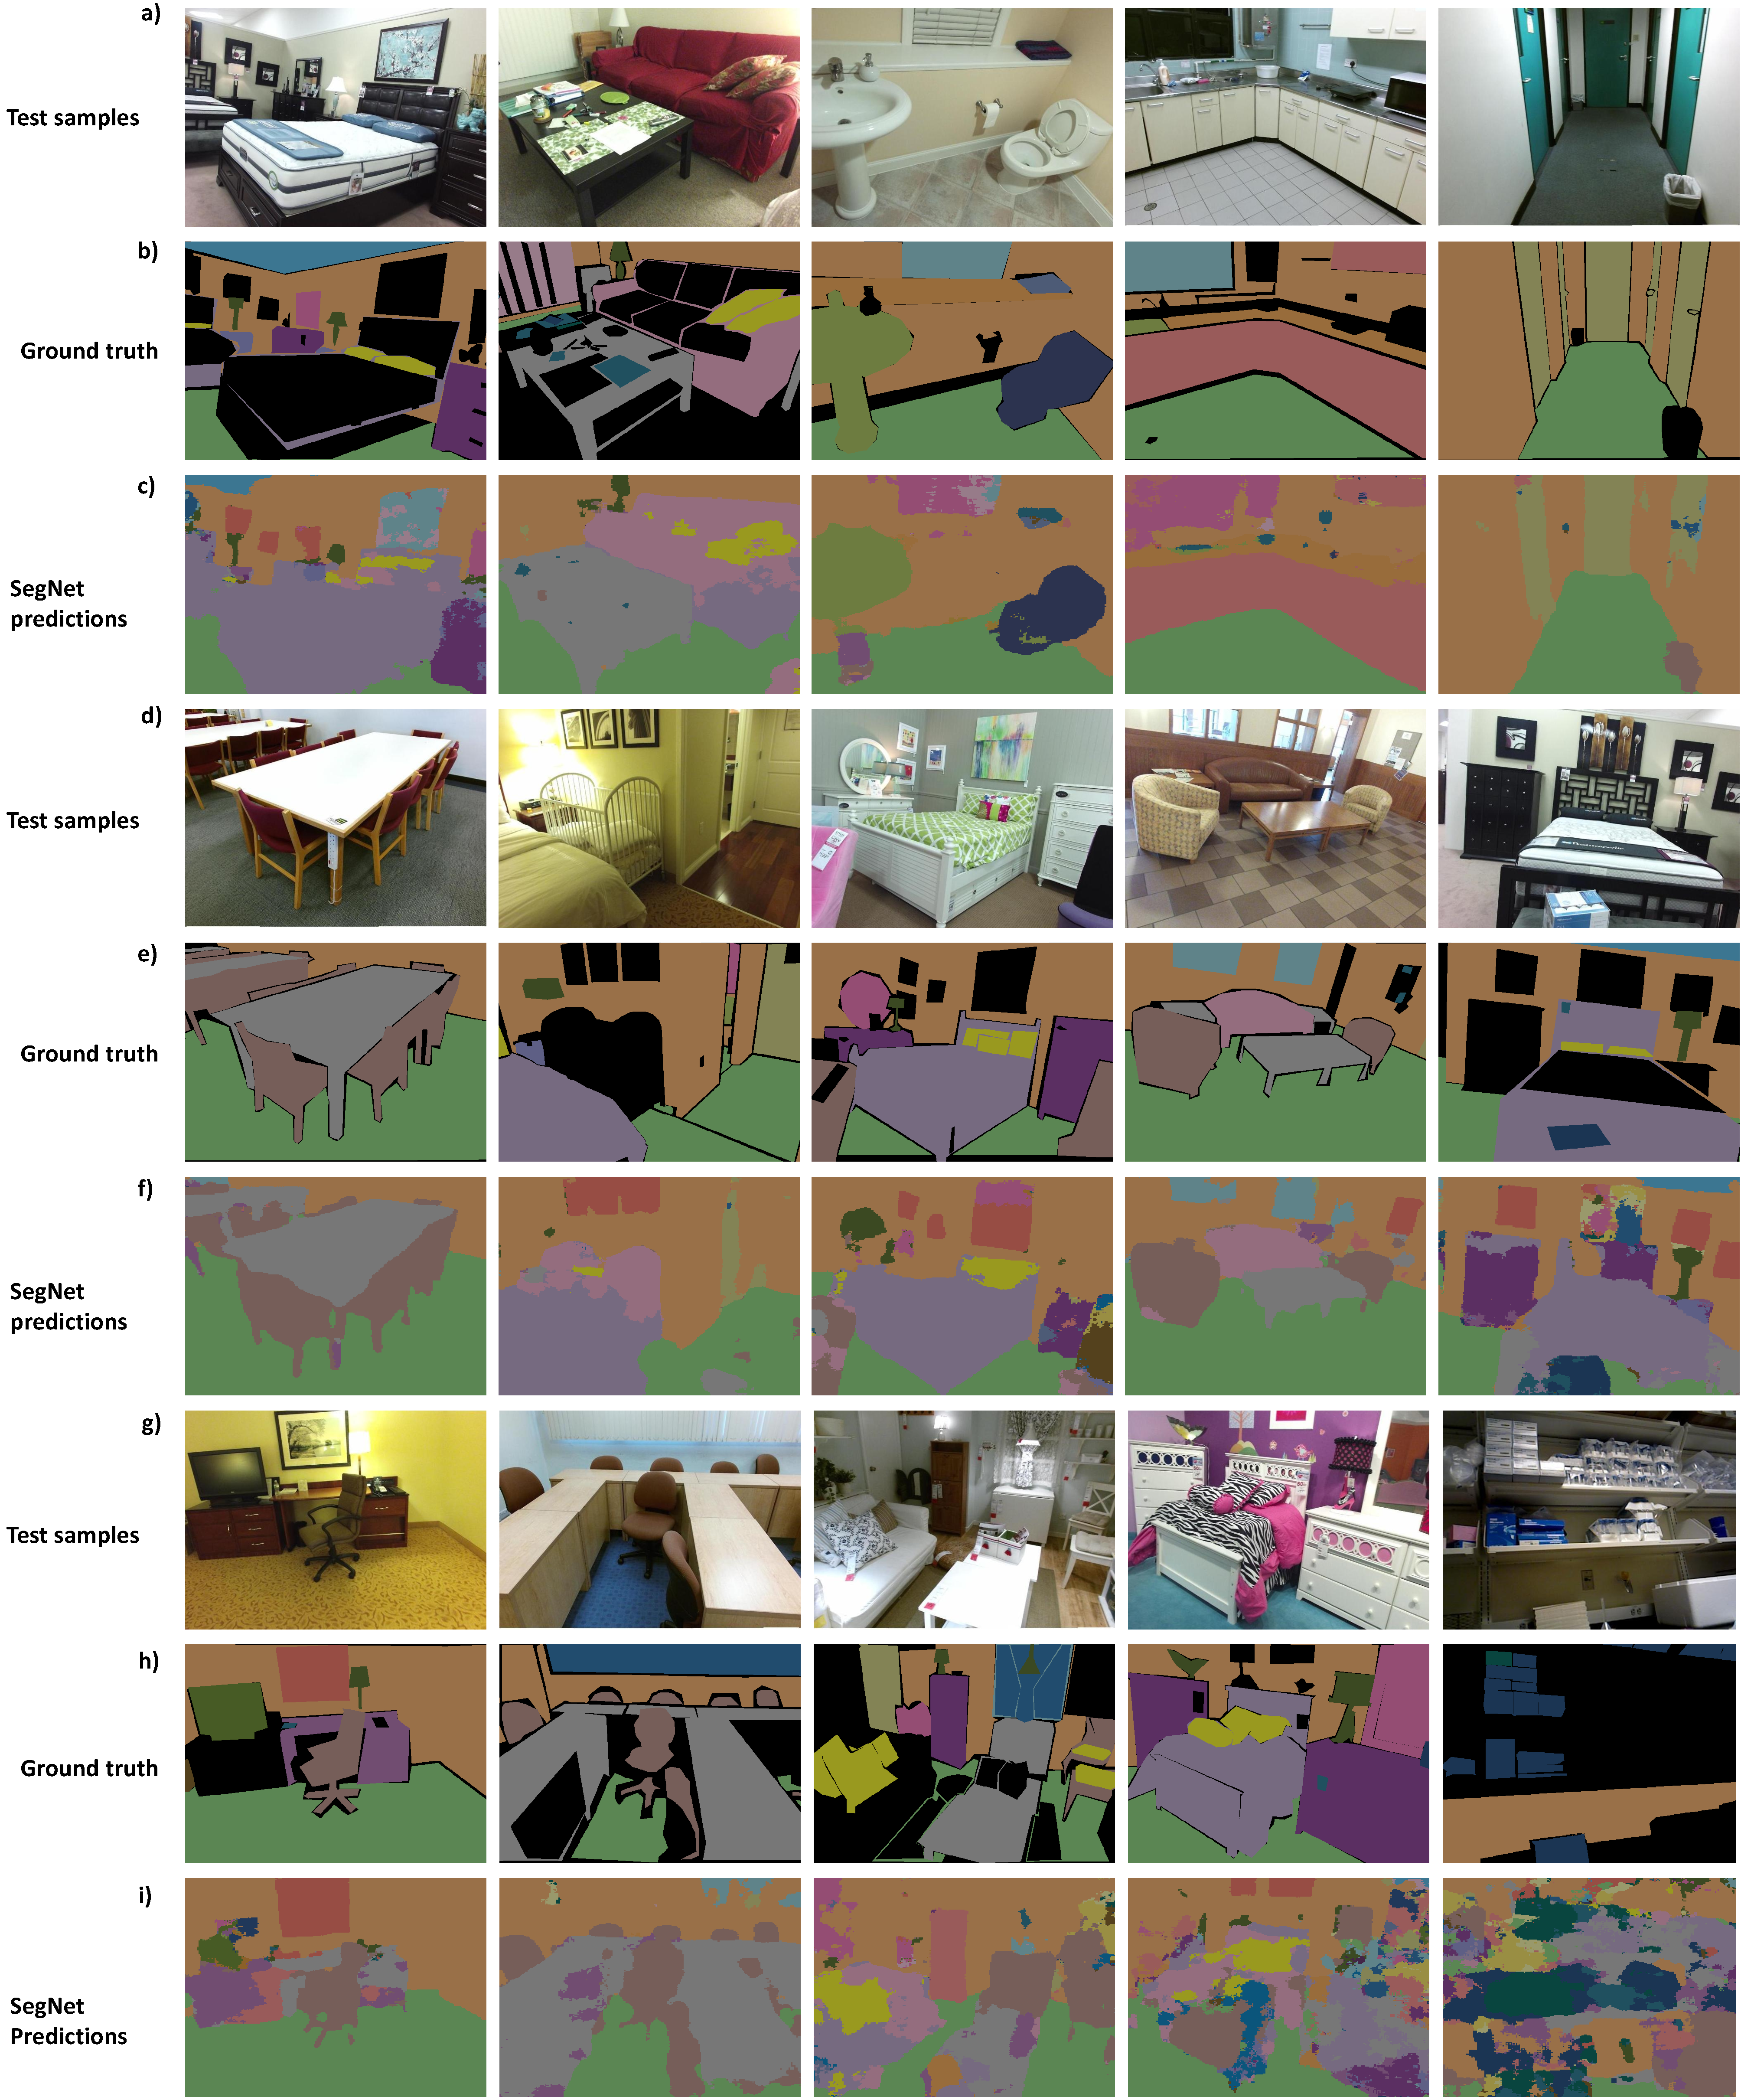
\includegraphics[width=\textwidth]{segnet/SUNRGBDQualy2.pdf}
\caption[SegNet qualitative results on RGB-D dataset.]{Qualitative assessment of SegNet predictions on RGB indoor test scenes from the recently released SUN RGB-D dataset \citep{song2015sun}. In this hard challenge, SegNet predictions delineate inter class boundaries well for object classes in a variety of scenes and their view-points. The segmentation quality is good when object classes are reasonably sized (rows (c,f)) but suffers when the scene is more cluttered (last two samples in row (i)). Unlabelled regions are shown as black in the ground truth.}
\label{SUNRGBDQualy}
\end{figure*}

Road scene images have limited variation, both in terms of the classes of interest and their spatial arrangements, especially when captured in a single sequence from a moving vehicle. In comparison, images of indoor scenes are more complex since the view points can vary significantly and there is less regularity in both the number of classes present in a scene and their spatial arrangement. Another difficulty is caused by the widely varying sizes of the object classes in the scene. Some test samples from the recent SUN RGB-D dataset \citep{song2015sun} are shown in \cref{SUNRGBDQualy}. We observe some scenes with few large classes and some others with dense clutter (bottom row and right). The appearance (texture and shape) can also widely vary in indoor scenes. Therefore, we believe this is the hardest challenge for segmentation architectures and methods in computer vision. Other challenges such as Pascal VOC12 \citep{pascal} salient object segmentation have occupied researchers more, but indoor scene segmentation is more challenging and has more practical applications such as in robotics. Our model advances state-of-the-art on the large SUN RGB-D dataset.

The qualitative results of SegNet on some images of indoor scenes of different types such as bedroom, kitchen, bathroom, classroom etc. are shown in \cref{SUNRGBDQualy}. We see that SegNet obtains sharp boundaries between classes when the scene consists of reasonable sized classes but even when view point changes are present (see bed segmentation from different view points). This is particularly interesting since the input modality is only RGB. It indicates the ability of SegNet to extract features from RGB images which are useful for view-point invariant segmentation provided there is sufficient training data (here 5285 images). RGB images are also useful to segment thinner structures such as the legs of chairs and tables, lamps which is difficult to achieve using depth images from currently available sensors. It is also useful to segment decorative objects such as paintings on the wall. 

In Table \ref{SUNRGBDtest} we report the quantitative results on the $37$ class segmentation task. We first note here that the other methods that have been benchmarked are not based on deep architectures and they only report class average accuracy. The existing top performing method \citep{ren2012rgb} relies on hand engineered features using colour, gradients and surface normals for describing super-pixels and then smooths super-pixel labels with a CRF. For SegNet we achieve a high global accuracy which correlates with an overall smooth segmentation. This also suggests that largest classes such as wall, floor, bed, table, sofa are segmented well in spite of view-point changes and appearance variations. However, the class average accuracy and mean IoU metric are poor, but at the same level as the hand engineered method which also includes the depth channel as input. This shows that smaller and thinner classes which have lesser training data are not segmented well. The individual class accuracies are reported in Table \ref{SUNRGBDClassavg}. From these we see that there is a clear correlation between the size and natural frequency of occurrence of classes and their individual accuracies. It is also informative to note RGB input is useful to segment widely varying (shape, texture) categories such as wall, floor, ceiling, table, chair, sofa with reasonable accuracy.

\begin{table}[t]
\centering
\begin{tabular}{c|ccc}
%\hline
{Method} & {Global avg.} & {Class avg.} & {Mean IoU} \\ \hline \hline
\multicolumn{4}{c}{RGB}                                                        \\ \hline
Liu \emph{et~al.}  \citep{SIFT_flow}      & n/a                  & 9.3                & n/a               \\ \hline
SegNet            & \textbf{70.3}                & 35.6               & \textbf{26.3}            \\ \hline
\multicolumn{4}{c}{RGB-D}                                                       \\ \hline
Liu \emph{et~al.}   \citep{SIFT_flow}    & n/a                  & 10.0               & n/a               \\ \hline
Ren et. al \citep{ren2012rgb}     & n/a                  & \textbf{36.3}               & n/a               \\ \hline
\end{tabular}
\caption[SegNet quantitative results on the SUN RGB-D dataset.]{Quantitative comparison on the SUN RGB-D dataset which consists of 5050 test images of indoor scenes with 37 classes. SegNet RGB based predictions have a high global accuracy and also matches the RGB-D based predictions \citep{ren2012rgb} in terms of class average accuracy.}
\label{SUNRGBDtest}
\end{table}

\begin{table*}[t]
\centering
\tabcolsep=3pt
 \resizebox{\textwidth}{!}{
\begin{tabular}{c|c|c|c|c|c|c|c|c|c|c|c|c}
%\hline
\multicolumn{1}{c|}{Wall} & \multicolumn{1}{c|}{Floor} & \multicolumn{1}{c|}{Cabinet} & \multicolumn{1}{c|}{Bed} & \multicolumn{1}{c|}{Chair} & \multicolumn{1}{c|}{Sofa} & \multicolumn{1}{c|}{Table} & \multicolumn{1}{c|}{Door} & \multicolumn{1}{c|}{Window} & \multicolumn{1}{c|}{Bookshelf} & \multicolumn{1}{c|}{Picture} & \multicolumn{1}{c|}{Counter} & \multicolumn{1}{c}{Blinds} \\ \hline
86.6                       & 92.0                       & 52.4                         & 68.4                     & 76.0                       & 54.3                      & 59.3                       & 37.4                      & 53.8                        & 29.2                           & 49.7                         & 32.5                         & 31.2                        \\ \hline
Desk                       & Shelves                    & Curtain                      & Dresser                  & Pillow                     & Mirror                    & Floor mat                  & Clothes                   & Ceiling                     & Books                          & Fridge                       & TV                           & Paper                       \\ \hline
17.8                       & 5.3                        & 53.2                         & 28.8                     & 36.5                       & 29.6                      & 0.0                        & 14.4                      & 67.7                        & 32.4                           & 10.2                         & 18.3                         & 19.2                        \\ \hline
Towel                      & Shower curtain             & Box                          & Whiteboard               & Person                     & Night stand               & Toilet                     & Sink                      & Lamp                        & Bathtub                        & Bag                          & \multicolumn{2}{c}{\multirow{2}{*}{}}                     \\ \cline{1-11}
11.5                       & 0.0                        & 8.9                          & 38.7                     & 4.9                        & 22.6                      & 55.6                       & 52.7                      & 27.9                        & 29.9                           & 8.1                          & \multicolumn{2}{c}{}                                      \\ \cline{1-11}
\end{tabular}}
\caption[SegNet class accuracy on SUN RGB-D.]{Class average accuracy of SegNet predictions for the 37 indoor scene classes in the SUN RGB-D benchmark dataset.}
\label{SUNRGBDClassavg}
\end{table*}

\subsubsection{Pascal VOC12 Segmentation Challenge}
\label{Pascal}
The Pascal VOC12 segmentation challenge \citep{pascal} consists of segmenting a few salient object classes from a widely varying background class. It is unlike the segmentation for scene understanding benchmarks described earlier which require learning both classes and their spatial context. A number of techniques have been proposed based on this challenge which are increasingly more accurate and complex.\footnote{\label{pascallb} See the leader board at \url{http://host.robots.ox.ac.uk:8080/leaderboard}} Our efforts in this benchmarking experiment have not been diverted towards attaining the top rank by either using multi-stage training \citep{long2015fully}, other datasets for pre-training such as MS-COCO \citep{lin2014microsoft, CRFRNN}, training and inference aids such as object proposals \citep{zitnick2014edge, NohDeconvNets} or post-processing using CRF based methods \citep{chen2016deeplab, NohDeconvNets}.  Although these supporting techniques clearly have value towards increasing the performance it unfortunately does not reveal the true performance of the deep architecture which is the \textit{core segmentation engine}. It however does indicate that some of the large deep networks are difficult to train end-to-end on this task even with pre-trained encoder weights. Therefore, to encourage more controlled benchmarking, we trained SegNet end-to-end without other aids and report this performance. 

In Table \ref{PascalQuant} we show the class average accuracy for some recent methods based on deep architectures. To the best of our ability, we have tried to gather the performance measures of the competing methods for their runs using minimum supporting techniques. We also specify when a method reports the performance of its core engine on the smaller validation set of $346$ images \citep{chen2016deeplab}. We find the performance on the full test set to be approximately  $1\%$ less as compared to the smaller validation set. 


\begin{figure*}[t]
\centering
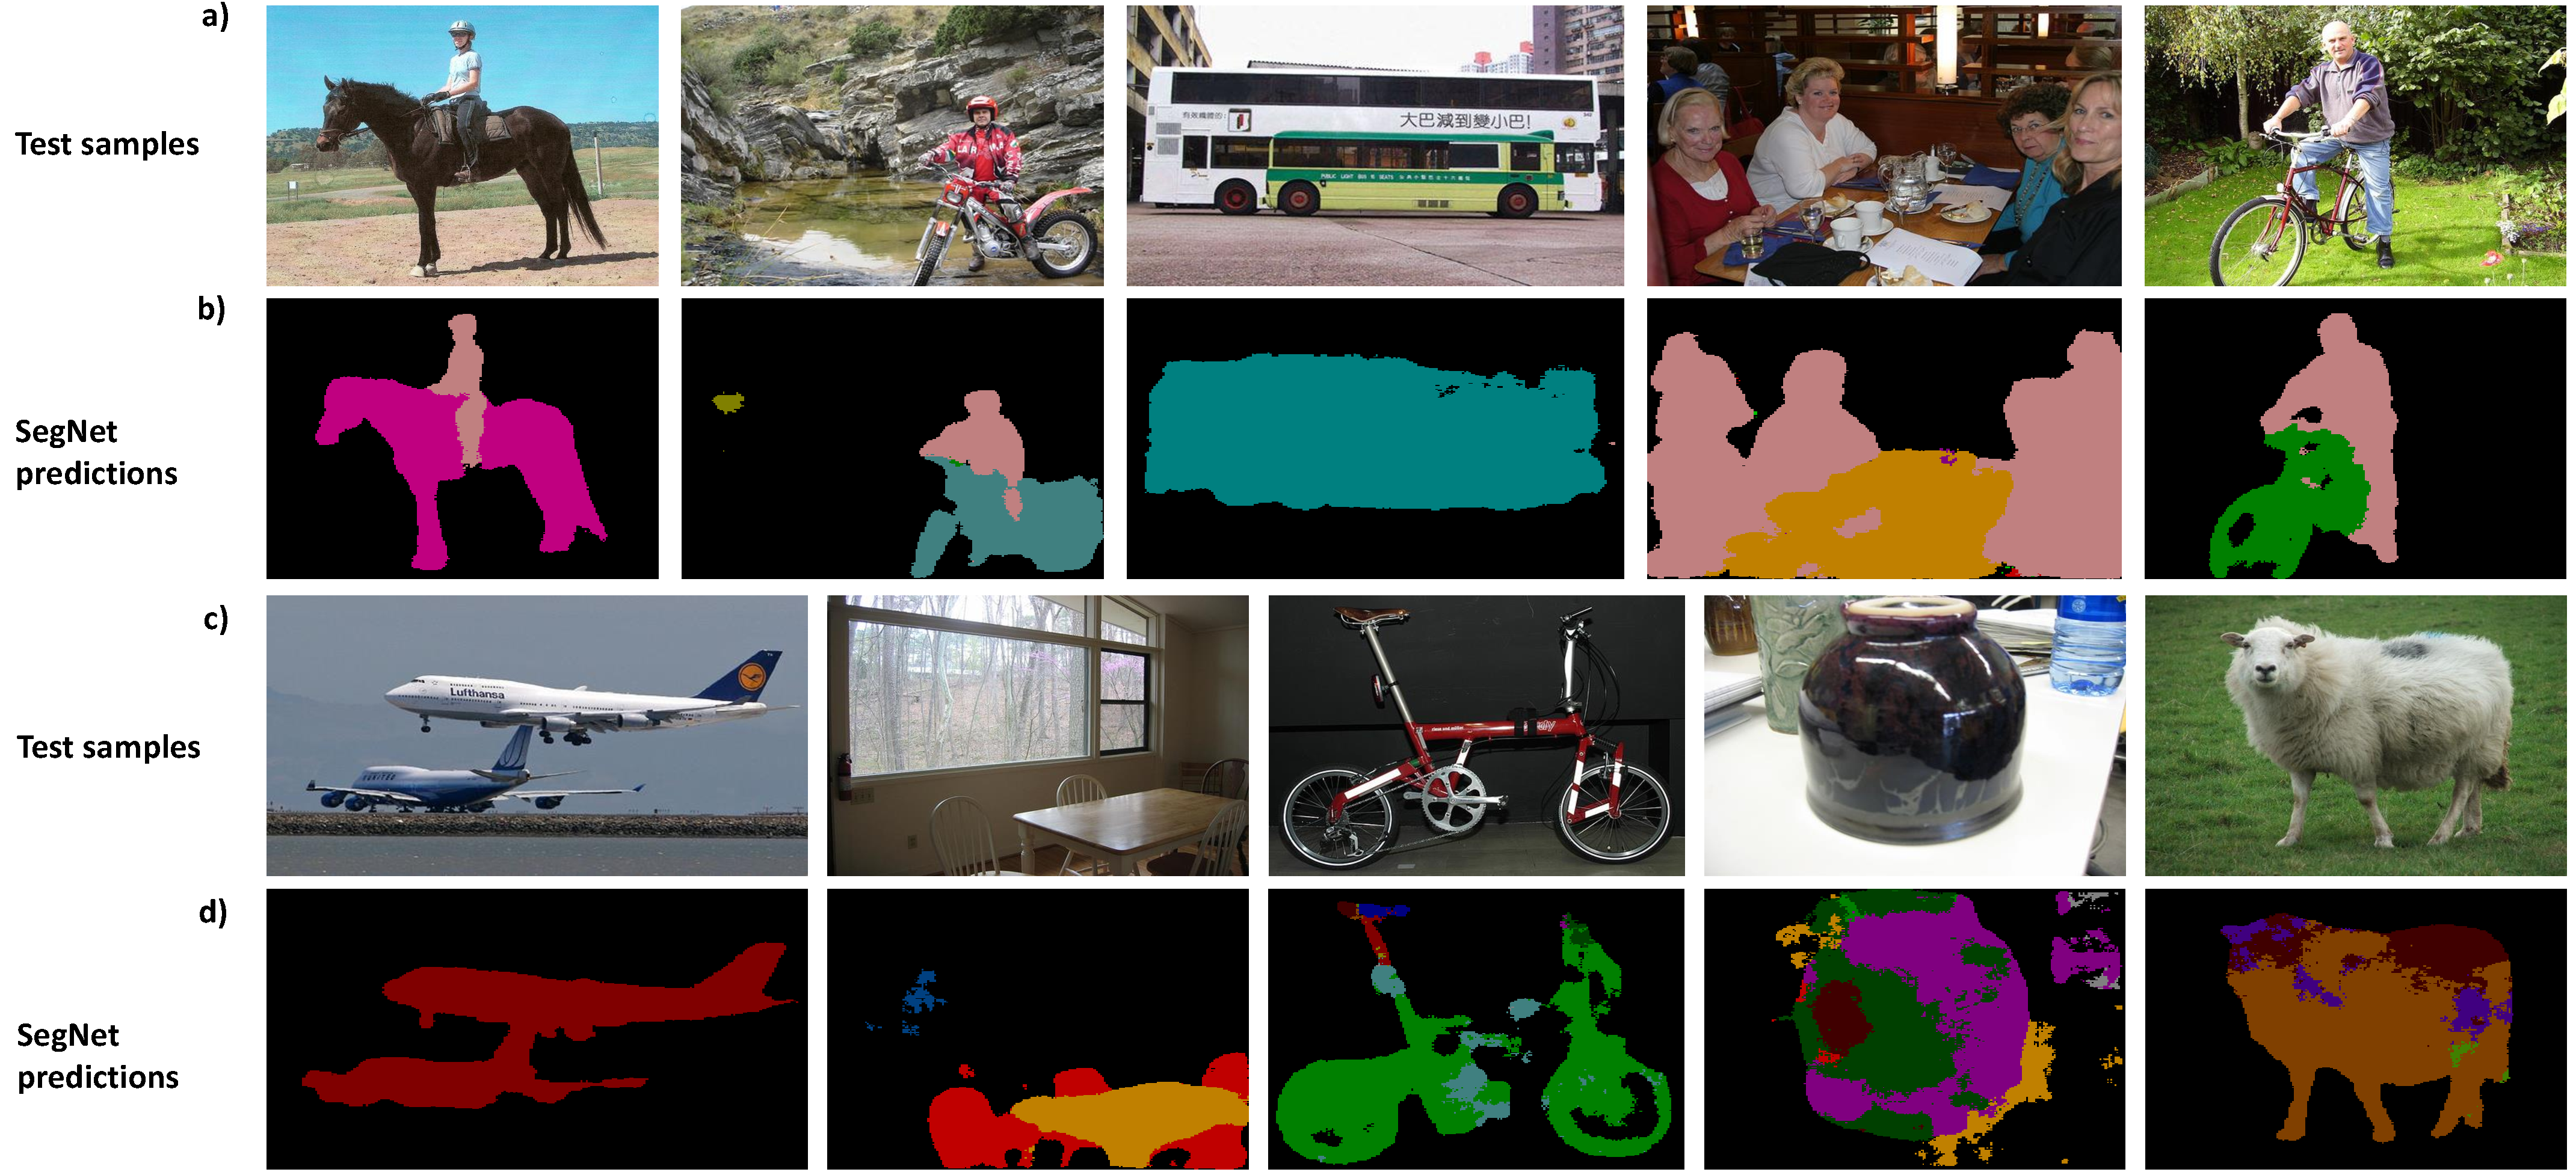
\includegraphics[width=\textwidth]{segnet/PascalQualy2.pdf}
\caption[Qualitative assessment of SegNet on Pascal VOC12]{Qualitative assessment of SegNet predictions on test samples from Pascal VOC12 \citep{pascal} dataset. SegNet performs competitively (row (b) on several object classes of varying shape and appearance. However, it lacks smoothness particularly on large objects (see row(d)). This can be perhaps be attributed to the smaller empirical size of the receptive field of the feature units in the deepest encoder layer size \citep{zhou2014object}.}
\label{PascalQualy}
\end{figure*}

\afterpage{%
    \begin{landscape}% Landscape page
\begin{table*}[]
\centering
\resizebox{\linewidth}{!}{
\tabcolsep=2pt
\begin{tabular}{c|c|c|c|c|c|c}
\hline
Method       & Encoder size (M) & Decoder size (M) & Total size (M) & Class avg. acc. & Inference $500 \times 500$ pixels & Inference $224 \times 224$ pixels \\ \hline \hline
chen2016deeplab \citep{chen2016deeplab} (validation set)  & n/a & n/a & $<$ 134.5 & 58   & n/a & n/a       \\ \hline
FCN-8 \citep{long2015fully}  (multi-stage training)  & 134 & \textbf{0.5} & 134.5 & 62.2  & 210ms & n/a       \\ \hline
Hypercolumns \citep{hariharan2015hypercolumns}  (object proposals) & n/a & n/a & $>$ 134.5 & 62.6  & n/a & n/a            \\ \hline
DeconvNet \citep{NohDeconvNets} (object proposals) &  138.35 & 138.35 & 276.7 & 69.6  & n/a & 92ms ($\times$ 50)        \\ \hline  
CRF-RNN \citep{CRFRNN} (multi-stage training)                  & n/a & n/a & $>$ 134.5 & \textbf{69.6} & n/a & n/a     \\ \hline
SegNet       & \textbf{14.725}       & 14.725 & \textbf{29.45} & 59.1   & \textbf{94ms}  & \textbf{28ms}  \\ \hline
\end{tabular}
}
\caption[SegNet performance on Pascal VOC 2012]{Quantitative comparison on Pascal VOC12 dataset. The accuracies for the competing architectures are gathered for their inference run using the least number of supporting training and inference techniques. However, since they are not trained end-to-end like SegNet and use aids such as object proposals, we have added corresponding qualifying comments. The first three columns show the number of trainable parameters in the encoder, decoder and full  network. Many of the models are approximately the same size as FCN. In comparison, SegNet is considerably smaller but achieves a competitive accuracy without resorting to supporting training or inference aids. This results in SegNet being significantly faster than other models in terms of inference time.}
\label{PascalQuant}
\end{table*}
\end{landscape}}

From the results in Table \ref{PascalQuant} we can see that the best performing networks are either very large (and slow) \citep{NohDeconvNets} and/or they use a CRF \citep{CRFRNN}. The CRF encourages large segments with a single label and this suits the Pascal challenge wherein there are one or two salient objects in the centre of the image. This prior also has a larger impact when training data is limited. This is shown in the experiments using CRF-RNN  \citep{CRFRNN} wherein the core FCN-8 model predictions are less accurate without extra training data. 

It is interesting that the DeepLab \citep{chen2016deeplab} architecture which is simply upsampling the FCN encoder features using bilinear interpolation performs reasonably well (on the validation set). The fact that a coarse segmentation is enough to produce this performance shows that this challenge is unlike scene understanding wherein many classes of varying shape and size need to be segmented.

Methods using object proposals during training and/or inference \citep{NohDeconvNets,hariharan2015hypercolumns} are very slow in inference time and it is hard to measure their true performance. These aids are necessitated by the very large size of their deep network \citep{NohDeconvNets} and also because the Pascal data can also be processed by a detect and segment approach. In comparison, SegNet is smaller by virtue of discarding the fully connected layers in the VGG16 \citep{simonyan2014very}. The authors of DeepLab \citep{chen2016deeplab} have also reported little loss in performance by reducing the size of the fully connected layers. The smaller size of SegNet makes end-to-end training possible for benchmarking. Although it may be argued that larger networks perform better, it is at the cost of a complex training mechanism, increased memory and inference time. This makes them unsuitable for real-time applications such as road scene understanding. 

The individual class accuracies for SegNet predictions on Pascal VOC12 are shown in Table \ref{PascalClassavg}. From this we once again see larger and more frequently occurring classes such as aeroplane, bus, cat \textit{etc}. have higher accuracy and smaller/thinner classes such as potted plant, bicycle are poorly segmented. We believe more training data \citep{lin2014microsoft} can help improve the performance of SegNet.

In the following section, we investigate techniques to improve our scene understanding algorithm by modelling uncertainty with deep learning.


\begin{table*}[t]
\centering
\resizebox{\linewidth}{!}{
\begin{tabular}{c|c|c|c|c|c|c|c|c|c|c}
\hline
Aeroplane & Bicycle & Bird & Boat & Bottle & Bus & Car & Cat & Chair & Cow & Dining table \\ \hline
74.5 & 30.6 & 61.4 & 50.8 & 49.8 & 76.2 & 64.3 & 69.7 & 23.8 & 60.8 & 54.7 \\ \hline
Dog  & Horse & Motor bike & Person & Potted plant & Sheep & Sofa & Train & TV & Background & \multirow{2}{*}{} \\ \cline{1-10}
62.0 & 66.4 & 70.2 & 74.1 & 37.5 & 63.7 & 40.6 & 67.8 & 53.0 & 88.6 & \\ \cline{1-10}
\end{tabular}}
\caption[Individual class accuracies of SegNet on Pascal VOC12]{Individual class accuracies of SegNet predictions on the Pascal VOC12 segmentation benchmark consisting of 21 object classes.}
\label{PascalClassavg}
\end{table*}









\section{Modelling Uncertainty}
\label{seg_unc}

The algorithms presented so far in this chapter produce accurate semantic segmentation predictions, however they are unaware of their uncertainty. Understanding what a model does not know is a critical part of many machine learning systems \citep{ghahramani2015probabilistic}.

Quantifying uncertainty in computer vision applications can be largely divided into regression settings such as depth regression, and classification settings such as semantic segmentation.
Existing approaches to model uncertainty in such settings in computer vision include particle filtering and conditional random fields \citep{blake1993framework, he2004multiscale}. However, many modern applications mandate the use of \textit{deep learning} to achieve state-of-the-art performance \citep{he2016deep}. Unfortunately most deep learning models not able to represent uncertainty.
For example, deep learning typically does not allow for uncertainty representation in regression settings. Deep learning classification models often give normalised score vectors, which do not necessarily capture model uncertainty. For both settings uncertainty can be captured with \textit{Bayesian deep learning} \citep{denker1991transforming, mackay1992practical, neal1995bayesian} approaches --
which offer a practical framework for understanding uncertainty with deep learning models 
\citep{gal2016thesis}.

In Bayesian modelling, there are two main types of uncertainty one can model \citep{der2009aleatory}. \textit{Aleatoric} uncertainty captures noise inherent in the observations.
This could be for example sensor noise or motion noise, resulting in uncertainty which cannot be reduced even if more data were to be collected.
On the other hand, \textit{epistemic} uncertainty accounts for uncertainty in the model parameters -- uncertainty which captures our ignorance about which model generated our collected data. 
This uncertainty can be explained away given enough data, and is often referred to as \textit{model uncertainty}. Aleatoric uncertainty can further be categorized into \textit{homoscedastic} uncertainty, uncertainty which stays constant for different inputs, and \textit{heteroscedastic} uncertainty. Heteroscedastic uncertainty depends on the inputs to the model, with some inputs potentially having more noisy outputs than others. 
Heteroscedastic uncertainty is especially important for computer vision applications. For example, for depth regression, highly textured input images with strong vanishing lines are expected to result in confident predictions, whereas an input image of a featureless wall is expected to have very high uncertainty.

In this section we make the observation that in many big data regimes (such as the ones common to deep learning with image data), it is most effective to model aleatoric uncertainty, uncertainty which cannot be explained away.
This is in comparison to epistemic uncertainty which is mostly explained away with the large amounts of data often available in machine vision.
We further show that modelling aleatoric uncertainty alone comes at a cost. Out-of-data examples, which can be identified with epistemic uncertainty, cannot be identified with aleatoric uncertainty alone.

For this we present a unified Bayesian deep learning framework which allows us to learn mappings from input data to aleatoric uncertainty and compose these together with epistemic uncertainty approximations. We derive our framework for both regression and classification applications and present results for per-pixel depth regression and semantic segmentation tasks (see \cref{fig:camvid_qual} for examples). 
We show how modelling aleatoric uncertainty in regression can be used to learn loss attenuation, and develop a complimentary approach for the classification case. 
This demonstrates the efficacy of our approach on difficult and large scale tasks.

The main contributions of this section are; 
\begin{enumerate}
\item We capture an accurate understanding of aleatoric and epistemic uncertainties, in particular with a novel approach for classification,
\item We improve model performance by $1-3\%$ over non-Bayesian baselines by reducing the effect of noisy data with the implied attenuation obtained from explicitly representing aleatoric uncertainty,
\item We study the trade-offs between modelling aleatoric or epistemic uncertainty by characterizing the properties of each uncertainty and comparing model performance and inference time.
\end{enumerate}

\begin{figure*}[t]
\centering
\resizebox{0.97\linewidth}{!}{
    \begin{subfigure}[t]{0.22\linewidth}
        \centering
		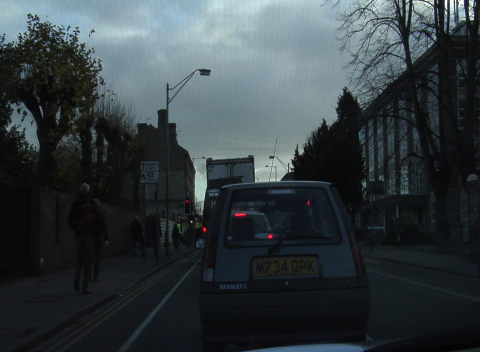
\includegraphics[width=\linewidth]{segnet_1_output_0.png}
        \vspace{1px}
		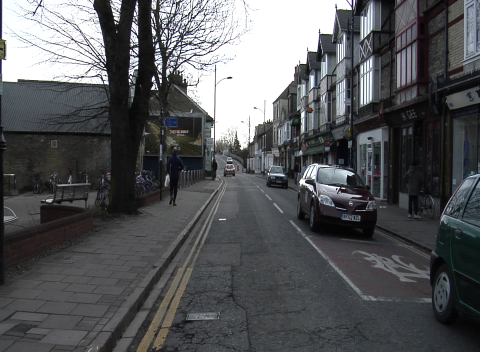
\includegraphics[width=\linewidth]{segnet_13_output_0.png}
        \vspace{1px}
        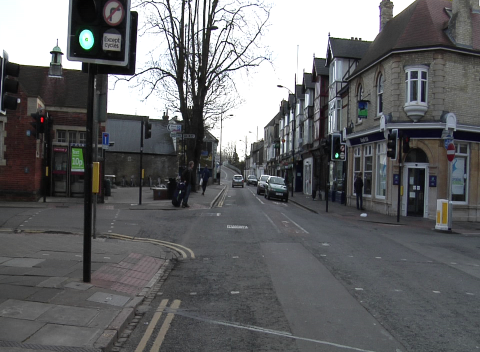
\includegraphics[width=\linewidth]{segnet_2_output_0.png}
        \caption{Input Image}
    \end{subfigure}
    \begin{subfigure}[t]{0.22\linewidth}
        \centering
		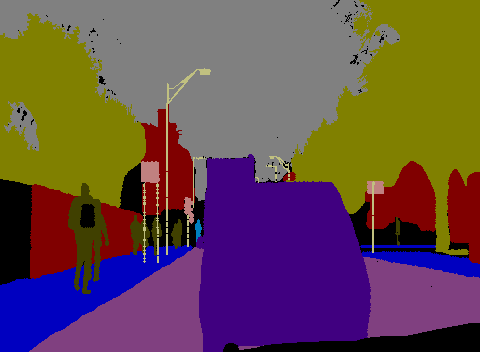
\includegraphics[width=\linewidth]{segnet_1_output_2.png}
        \vspace{1px}
		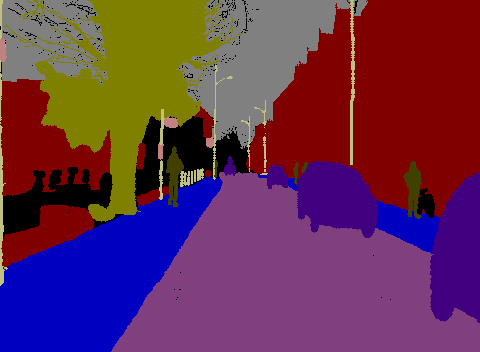
\includegraphics[width=\linewidth]{segnet_13_output_2.png}
        \vspace{1px}
        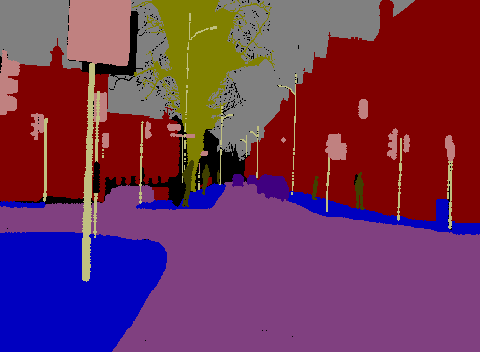
\includegraphics[width=\linewidth]{segnet_2_output_2.png}
        \caption{Ground Truth}
    \end{subfigure}
    \begin{subfigure}[t]{0.22\linewidth}
        \centering
		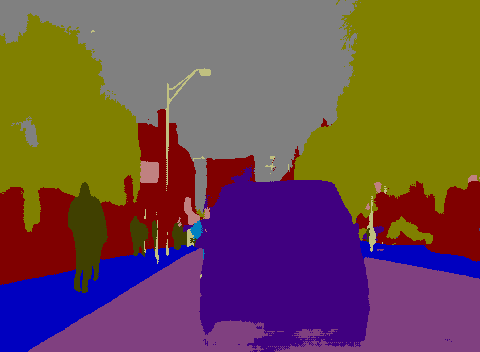
\includegraphics[width=\linewidth]{segnet_1_output_1.png}
        \vspace{1px}
		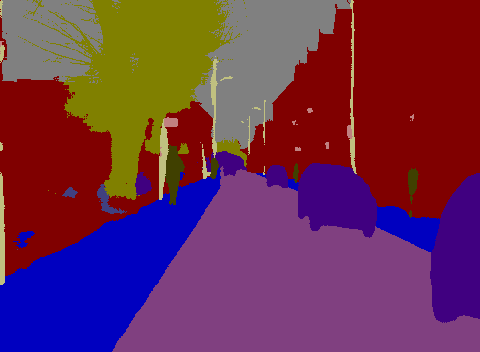
\includegraphics[width=\linewidth]{segnet_13_output_1.png}
        \vspace{1px}
        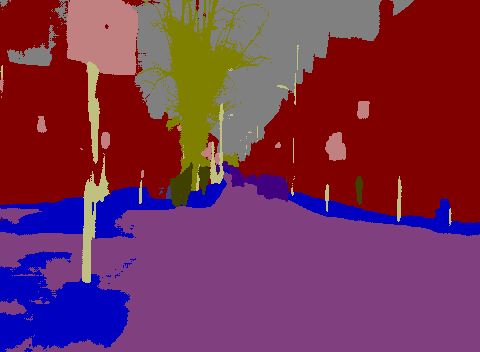
\includegraphics[width=\linewidth]{segnet_2_output_1.png}
        \caption{Semantic\\Segmentation}
    \end{subfigure}
    \begin{subfigure}[t]{0.22\linewidth}
        \centering
		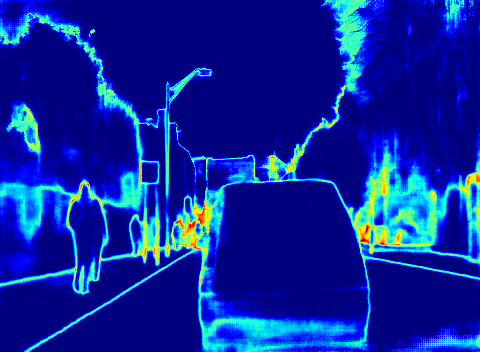
\includegraphics[width=\linewidth]{segnet_1_output_3.png}
        \vspace{1px}
		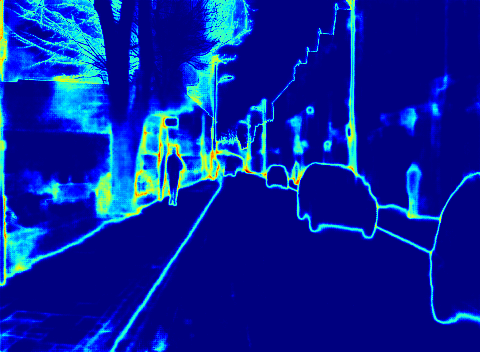
\includegraphics[width=\linewidth]{segnet_13_output_3.png}
        \vspace{1px}
        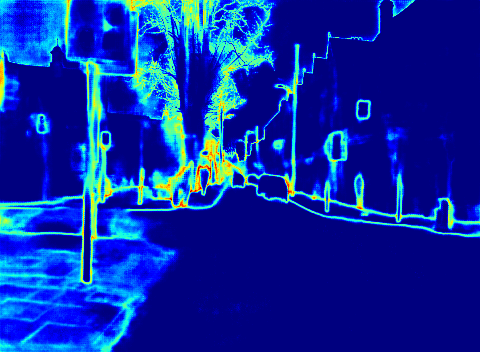
\includegraphics[width=\linewidth]{segnet_2_output_3.png}
        \caption{Aleatoric\\Uncertainty}
    \end{subfigure}
    \begin{subfigure}[t]{0.22\linewidth}
        \centering
		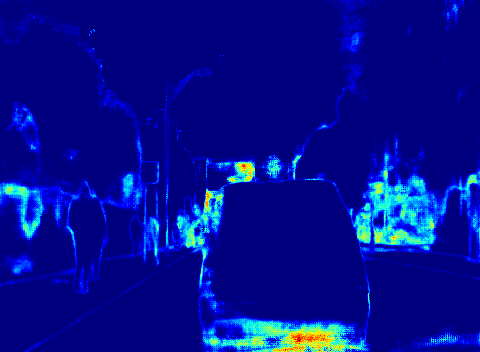
\includegraphics[width=\linewidth]{segnet_1_output_5.png}
        \vspace{1px}
		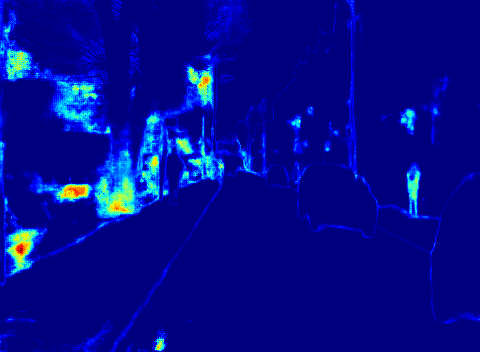
\includegraphics[width=\linewidth]{segnet_13_output_5.png}
        \vspace{1px}
        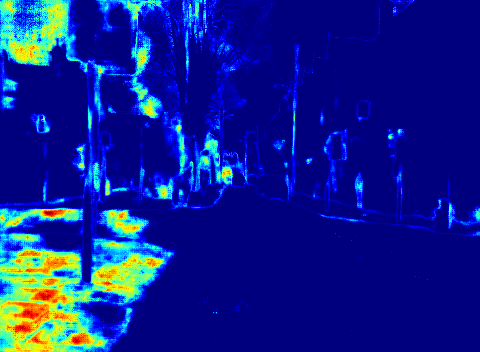
\includegraphics[width=\linewidth]{segnet_2_output_5.png}
        \caption{Epistemic\\Uncertainty}

\end{subfigure}}
\caption[Comparing different types of uncertainty in deep learning.]{\textbf{Illustrating the difference between aleatoric and epistemic uncertainty} for semantic segmentation on the CamVid dataset \citep{brostow2009semantic}. We observe aleatoric uncertainty captures object boundaries where labels are noisy. The bottom row shows a failure case of the segmentation model, when the model fails to segment the footpath, and the corresponding increased epistemic uncertainty.}
\label{fig:camvid_qual}
\end{figure*}

\subsection{Bayesian Deep Learning}
\label{related_work}

Existing approaches to Bayesian deep learning capture either epistemic uncertainty alone, or aleatoric uncertainty alone \citep{gal2016thesis}. These uncertainties are formalised as probability distributions over either the model parameters, or model outputs, respectively. Epistemic uncertainty is modelled by placing a prior distribution over a model's weights, and then trying to capture how much these weights vary given some data. Aleatoric uncertainty on the other hand is modelled by placing a distribution over the output of the model. For example, in regression our outputs might be modelled as corrupted with Gaussian random noise. In this case we are interested in learning the noise's variance as a function of different inputs (such noise can also be modelled with a constant value for all data points, but this is of less practical interest). These uncertainties, in the context of Bayesian deep learning, are explained in more detail in this section. 

\subsection{Epistemic Uncertainty in Bayesian Deep Learning}
\label{sect:dropout_VI}

To capture epistemic uncertainty in a neural network (NN) we put a prior distribution over its weights, for example a Gaussian prior distribution:
$\W \sim \N(0, I)$.

Such a model is referred to as a Bayesian neural network (BNN) \citep{ denker1991transforming, mackay1992practical, neal1995bayesian}. 
Bayesian neural networks replace the deterministic network's weight parameters with distributions over these parameters, and instead of optimising the network weights directly we average over all possible weights (referred to as \textit{marginalisation}). 
% (or optimise the parameters of the distributions (or integrate ) instead of .
Denoting the random output of the BNN as $\f^\W(\x)$, we define the model likelihood $p(\y | \f^\W(\x))$.
Given a dataset $\X=\{\x_1, ..., \x_N\}$, with labels $\Y=\{\y_1, ..., \y_N\}$, Bayesian inference is used to compute the posterior over the weights $p(\W | \X, \Y)$. This posterior captures the set of plausible model parameters, given the data.

For regression tasks we often define our likelihood as a Gaussian with mean given by the model output:
$
p(\y | \f^\W(\x)) = \N(\f^\W(\x), \sigma^2)
$,
with an observation noise scalar $\sigma$. 
For classification, on the other hand, we often squash the model output through a softmax function, and sample from the resulting probability vector:
% \newcommand{\softmax}{\text{softmax}}
$
p(\y | \f^\W(\x)) = \softmax(\f^\W(\x))
$.

BNNs are easy to formulate, but difficult to perform inference in. This is because the marginal probability $p(\Y | \X)$, required to evaluate the posterior,
\begin{equation}  
p(\W | \X, \Y) = \frac{p(\Y | \X, \W)p(\W)}{p(\Y | \X)},
\end{equation}  
cannot be evaluated analytically. Different approximations exist \citep{graves2011practical, blundell2015weight, hernandez2016black, Gal2016Bayesian}.
In these approximate inference techniques, the posterior $p(\W | \X, \Y)$ is fitted with a simple distribution $q_\theta^*(\W)$, parametrised by $\theta$. This replaces the intractable problem of averaging over all weights in the BNN with an optimisation task, where we seek to optimise over the \textit{parameters of the simple distribution} instead of optimising the original neural network's parameters.

Dropout variational inference is a practical approach for approximate inference in large and complex models \citep{Gal2016Bayesian}. 
This inference is done by training a model with dropout before every weight layer, and by also performing dropout at test time to sample from the approximate posterior (stochastic forward passes, referred to as Monte Carlo dropout).
More formally, this approach is equivalent to performing approximate variational inference where we find a simple distribution $q_\theta^*(\W)$ in a tractable family which minimises the Kullback-Leibler (KL) divergence to the true model posterior $p(\W | \X, \Y)$. 
Dropout can be interpreted as a variational Bayesian approximation, where the approximating distribution is a mixture of two Gaussians with small variances and the mean of one of the Gaussians is fixed at zero. 
%
The minimisation objective is given by \citep{jordan1999introduction}:
% \newcommand{\cL}{\mathcal{L}}
\begin{equation}  
\cL(\theta, p) = - \frac{1}{N} \sum_{i=1}^N \log p(\y_i | \f^{\Wh_i}(\x_i)) + \frac{1 - p}{2N} ||\theta||^2
\end{equation}
with $N$ data points, dropout probability $p$, samples $\Wh_i \sim q_\theta^*(\W)$, and $\theta$ the set of the simple distribution's parameters to be optimised (weight matrices in dropout's case). In regression, for example, the negative log likelihood can be further simplified as
\begin{equation}
-\log p(\y_i | \f^{\Wh_i}(\x_i)) \propto  \frac{1}{2 \sigma^2}||\y_i - \f^{\Wh_i}(\x_i)||^2 + \frac{1}{2} \log \sigma^2
\end{equation}
for a Gaussian likelihood,
% or 
% \begin{align*}
% -\log p(\y_i | \f^{\Wh_i}(\x_i)) \propto \frac{1}{\sigma^2}||\y_i - \f^{\Wh_i}(\x_i)|| + \log \sigma^2 
% \end{align*}
% for a Laplace likelihood,
with $\sigma$ the model's observation noise parameter -- capturing how much noise we have in the outputs.

Epistemic uncertainty in the weights can be reduced by observing more data. This uncertainty induces prediction uncertainty by marginalising over the (approximate) weights posterior distribution. For classification this can be approximated using Monte Carlo integration as follows:
\begin{equation}
p(y=c | \x, \X, \Y) 
% &= \int p(y=c | \x, \W) p(\W | \X, \Y) \td \W \\
% &\approx 
% \int p(y=c | \x, \W) q_\theta^*(\W) \td \W \\
% &\approx 
% \frac{1}{T} \sum_{t=1}^T p(y=c | \x, \Wh_t) \\
% &=
\approx
\frac{1}{T} \sum_{t=1}^T \softmax(\f^{\Wh_t}(\x))
\end{equation}
with $T$ sampled masked model weights $\Wh_t \sim q_\theta^*(\W)$, where $q_\theta(\W)$ is the Dropout distribution \citep{gal2016thesis}. 
The uncertainty of this probability vector $\p$ can then be summarised using the entropy of the probability vector:
$H(\p) = - \sum_{c=1}^C p_c \log p_c.$
For regression this epistemic uncertainty is captured by the predictive variance, which can be approximated as:
\begin{equation}
\text{Var}(\y) \approx \sigma^2 + \frac{1}{T} \sum_{t=1}^T \f^{\Wh_t}(\x)^T \f^{\Wh_t}(\x_t) - E(\y)^T E(\y)
\end{equation}
with predictions in this epistemic model done by approximating the predictive mean: 
$E(\y) \approx \frac{1}{T} \sum_{t=1}^T \f^{\Wh_t}(\x).$
The first term in the predictive variance, $\sigma^2$, corresponds to the amount of noise inherent in the data (heteroscedastic noise -- which will be explained in more detail soon). The second part of the predictive variance measures how much the model is uncertain about its predictions -- this term will vanish when we have zero parameter uncertainty (i.e.\ when all draws $\Wh_t$ take the same constant value). 

\subsection{Heteroscedastic Aleatoric Uncertainty}
\label{sect:hetero}

In the above we captured model uncertainty -- uncertainty over the model parameters -- by approximating the distribution $p(\W | \X, \Y)$. To capture aleatoric uncertainty in regression, we would have to tune the observation noise parameter $\sigma$.

Homoscedastic regression assumes constant observation noise $\sigma$ for every input point $\x$. Heteroscedastic regression, on the other hand, assumes that observation noise can vary with input $\x$ \citep{nix1994estimating, le2005heteroscedastic}. Heteroscedastic models are useful in cases where parts of the observation space might have higher noise levels than others.
In non-Bayesian neural networks, this observation noise parameter is often fixed as part of the model's weight decay, and ignored. However, when made data-dependent, it can be learned as a function of the data:
\begin{equation}
\cL_\text{NN}(\theta) = \frac{1}{N} \sum_{i=1}^N \frac{1}{2\sigma(\x_i)^2} ||\y_i - \f(\x_i)||^2 + \frac{1}{2} \log \sigma(\x_i)^2 %+ \lambda ||\theta||^2
% \cL(\theta, p) = \frac{1}{N} \sum_{i=1}^N \log \frac{1}{\sigma(\x_i)^2}||\y_i - \f^{\Wh_i}(\x_i)||^2 + \log \sigma(\x_i)^2 + \frac{1 - p}{N} ||\theta||^2.
\end{equation}
% \red{TODO: change Gaussian to Laplace likelihood}
with added weight decay parametrized by $\lambda$ (and similarly for $l_1$ loss).
Note that here, unlike the above, variational inference is \textit{not} performed over the weights, but instead we perform maximum a posteriori (MAP) inference -- finding a single value for the model parameters $\theta$. This approach \textit{does not} capture epistemic model uncertainty, as epistemic uncertainty is a property of the model and not of the data.

In the next section we will combine these two types of uncertainties together in a single model. We will see how heteroscedastic noise can be interpreted as model attenuation, and develop a complimentary approach for the classification case. %We will study how each uncertainty affects the models trained.


\subsection{Combining Aleatoric and Epistemic Uncertainty in One Model}
\label{sec:method}

In the previous section we described existing Bayesian deep learning techniques. In this section we present novel contributions which extend this existing literature. We develop models that will allow us to study the effects of modelling either aleatoric uncertainty alone, epistemic uncertainty alone, or modelling both uncertainties together in a single model. This is followed by an observation that aleatoric uncertainty in regression tasks can be interpreted as learned loss attenuation -- making the loss more robust to noisy data. We follow that by extending the ideas of heteroscedastic regression to classification tasks. This allows us to learn loss attenuation for classification tasks as well. %, and obtain improved aleatoric uncertainty estimates in classification.


We wish to capture both epistemic and aleatoric uncertainty in a vision model.
For this we turn the heteroscedastic neural network in \cref{sect:hetero} into a Bayesian neural network by placing a distribution over its weights, with our construction in this section developed specifically for the case of vision models\footnote{Although this construction can be generalised for any heteroscedastic neural network architecture.}.

We need to infer the posterior distribution for a BNN model $\f$ mapping an input image, $\x$, to a unary output, $\hat{\y} \in \mathbb{R}$, and a measure of aleatoric uncertainty given by variance, $\mathbf{\sigma}^2$. We approximate the posterior over the BNN with a dropout variational distribution using the tools of \cref{sect:dropout_VI}. 
As before, we draw model weights from the approximate posterior $\Wh \sim q(\W)$ to obtain a model output, this time composed of both predictive mean as well as predictive variance:
\begin{equation}
[\hat{\y}, \hat{\mathbf{\sigma}}^2] = \f^{\Wh}(\textbf{x})
\end{equation}
where $\f$ is a Bayesian convolutional neural network parametrised by model weights $\Wh$. We can use a single network to transform the input $\x$, with its head split to predict both $\hat{\y}$ as well as $\hat{\sigma}^2$.

% For regression tasks we train our network to learn a continuous valued function and predict the unaries $x_i \in \mathbb{R}$. 
We fix a Gaussian likelihood to model our aleatoric uncertainty.
This induces a minimisation objective given labelled output points $x$:
\begin{equation}
\cL_{BNN}(\theta) = \frac{1}{D} \sum_i \frac{1}{2} \hat{\sigma}^{-2}_i ||\y_i-\hat{\y}_i||^2 + \frac{1}{2} \log{\hat{\sigma}_i^2}
\end{equation}
where $D$ is the number of output pixels $\y_i$ corresponding to input image $\x$, indexed by i (additionally, the loss includes weight decay which is omitted for brevity). For example, we may set $D=1$ for image-level regression tasks, or $D$ equal to the number of pixels for dense prediction tasks (predicting a unary corresponding to each input image pixel). $\hat{\sigma}^2_i$ is the BNN output for the predicted variance for pixel $i$.

This loss consists of two components; the residual regression obtained with a stochastic sample through the model -- making use of the uncertainty over the parameters  -- and an uncertainty regularization term. We do not need `uncertainty labels' to learn uncertainty. Rather, we only need to supervise the learning of the regression task. We learn the variance, $\sigma^2$, implicitly from the loss function. The second regularization term prevents the network from predicting infinite uncertainty (and therefore zero loss) for all data points.

In practice, we train the network to predict the log variance, $s_i := \log \hat{\sigma}_i^2$: 
\begin{equation}
\cL_{BNN}(\theta) = \frac{1}{D} \sum_i \frac{1}{2} \exp (-s_i) ||\y_i-\hat{\y}_i||^2 + \frac{1}{2} s_i.
\label{eqn:aleatoric_regression_loss}
\end{equation}
This is because it is more numerically stable than regressing the variance, $\sigma^2$, as the loss avoids a potential division by zero. The exponential mapping also allows us to regress unconstrained scalar values, where $\exp(-s_i)$ is resolved to the positive domain giving valid values for variance.

% Following the notation of the previous section, the predictive uncertainty in this combined model can be approximated using:
% \begin{align*}
% \text{Var}(\y) &\approx \frac{1}{T} \sum_{t=1}^T \f^{\Wh_t}(\x)^T \f^{\Wh_t}(\x_t)
% - E(\y)^T E(\y) \\
% &\qquad + \frac{1}{T} \sum_{t=1}^T (\sigma^{\Wh_t}(\x))^2.
% \end{align*}
To summarize, the predictive uncertainty for pixel $\y$ in this combined model can be approximated using:
\begin{equation}
\text{Var}(\y) \approx \frac{1}{T} \sum_{t=1}^T \hat{\y}_{t}^2
- \bigg( \frac{1}{T} \sum_{t=1}^T \hat{\y}_{t} \bigg)^2 + \frac{1}{T} \sum_{t=1}^T \hat{\sigma}_{t}^2
\end{equation}
with $\{ \hat{\y}_{t}, \hat{\sigma}_{t}^2 \}_{t=1}^T$ a set of $T$ sampled outputs: $\hat{\y}_{t}, \hat{\sigma}_{t}^2 = \f^{\Wh_t}(\x)$ for randomly masked weights $\Wh_t \sim q(\W)$.


\subsection{Heteroscedastic Uncertainty as Learned Loss Attenuation}

We observe that allowing the network to predict uncertainty, allows it effectively to temper the residual loss by $\exp(-s_i)$, which depends on the data. This acts similarly to an intelligent robust regression function. It allows the network to adapt the residual's weighting, and even allows the network to learn to attenuate the effect from erroneous labels. This makes the model more robust to noisy data: inputs for which the model learned to predict high uncertainty will have a smaller effect on the loss.

The model is discouraged from predicting high uncertainty for all points -- in effect ignoring the data -- through the $\log \sigma^2$ term. Large uncertainty increases the contribution of this term, and in turn penalizes the model: The model \textit{can} learn to ignore the data -- but is penalised for that. The model is also discouraged from predicting very low uncertainty for points with high residual error, as low $\sigma^2$ will exaggerate the contribution of the residual and will penalize the model. It is important to stress that this learned attenuation is not an ad-hoc construction, but a consequence of the probabilistic interpretation of the model. 

This learned loss attenuation property of heteroscedastic neural networks in regression is a desirable effect for classification models as well. 
However, heteroscedastic neural networks in classification are peculiar models because technically any classification task has input-dependent uncertainty. Nevertheless, the ideas above can be extended from regression heteroscedastic networks to classification heteroscedastic networks, which we discuss.


\subsection{Heteroscedastic Uncertainty in Classification Tasks}

We extend the results above to classification models, allowing us to get the equivalent of the learned loss attenuation property in classification as well.
For this we adapt the standard classification model to marginalise over intermediate heteroscedastic regression uncertainty placed over the \textit{logit space}.
We therefore explicitly refer to our proposed model adaptation as a \textit{heteroscedastic} classification neural network.

For classification tasks our model predicts a vector of unaries $\f_i$ for each pixel $i$, which when passed through a softmax operation, forms a probability vector $\p_i$. We change the model by placing a Gaussian distribution over the unaries vector:
\begin{equation}
\begin{split}
\hat{\x}_i | \W \sim \N(\f^\W_i, (\sigma_i^\W)^2)
\\
\hat{\p}_i = \softmax(\hat{\x}_i).
\end{split}
\end{equation}
Here $\f^\W_i, \sigma_i^\W$ are the network outputs with parameters $\W$.
This vector $\f^\W_i$ is corrupted with Gaussian noise with variance $(\sigma_i^\W)^2$ (a diagonal matrix with one element for each logit value), and the corrupted vector is then squashed with the softmax function to obtain $\p_i$, the probability vector for pixel $i$.

Our expected log likelihood for this model is given by:
\begin{equation}
E_{\N(\hat{\x}_i; \f^\W_i, (\sigma_i^\W)^2)}[\log \hat{\p}_{i,c}]
\end{equation}
with $c$ the observed class for input $i$,
which gives us our loss function.
Ideally, we would want to analytically integrate out this Gaussian distribution, but no analytic solution is known.
We therefore approximate the objective through Monte Carlo integration, and sample unaries through the softmax function.
We note that this operation is extremely fast because we perform the computation once (passing inputs through the model to get logits). We only need to sample from the logits, which is a fraction of the network's compute, and therefore does not significantly increase the model's test time. 
We can rewrite the above and obtain the following numerically-stable stochastic loss:
\begin{equation}
\begin{split}
\hat{\x}_{i,t} &= \f^\W_i + \epsilon_t, \quad \epsilon_t \sim \mathcal{N}(0,\,(\sigma_i^\W)^2)
\\
\cL_x &= \frac{1}{T} \sum_{i,t} (- \hat{x}_{i,t,c} + \log \sum_{c'} \exp \hat{x}_{i,t,c'})
\end{split}
\label{eqn:aleatoric_classification_loss}
\end{equation}
with $x_{i,t,c'}$ the $c'$ element in the logit vector $\x_{i,t}$. 

This objective can be interpreted as learning loss attenuation, similarly to the regression case.
To understand this objective, we concentrate on a single pixel $i$ and reformulate the objective as $\sum_{t} \log \sum_{c'} \exp (\hat{x}_{t,c'} - \hat{x}_{t,c})$ with $c$ the observed class and $t$ Gaussian samples. We shall analyse what this objective behaves like for various settings.
When the model gives the observed class a high logit value $f_{c}$ (compared to the logit values of other classes) and a low noise value $\sigma_{c}$, this loss will be near zero -- the ideal case. When the model attempts to give the observed class a low logit value (for example if the label is noisy and $f_{c'}$ is the highest logit for some incorrect $c' \neq c$), there are two cases of interest. If the observed class logit has a low noise value, then the loss will be penalised by approximately $f_{c'} - f_{c}$\footnote{To see this, pull the term $f_{c'} - f_{c}$ out of the log-sum-exp; the corresponding exponent will now be $\exp(0)=1$, and since this was the largest exponent, the remaining exp terms in the sum will be near zero.}. However, if the model increases the noise value for this last case, then some noise samples will take a high value and the penalisation will be decreased from this last quantity. Lastly, the model is discouraged from increasing the noise when the observed class is given a high logit value. This is because large noise would lead some logit samples to take high negative values, and these samples will increase the loss.


We next assess the above ideas empirically.


\subsection{Experiments}
\label{sec:results}

In this section we evaluate our methods with pixel-wise depth regression and semantic segmentation. An analysis of these results is given in the following section. To show the robustness of our learned loss attenuation -- a side-effect of modelling uncertainty -- we present results on an array of popular datasets, CamVid \citep{brostow2009semantic}, Make3D \citep{saxena2009make3d}, and NYUv2 Depth \citep{silberman2012indoor}, where we advance state-of-the-art.


For the following experiments we use the DenseNet architecture \citep{huang2016densely} which has been adapted for dense prediction tasks by \citep{jegou2016one}. We use our own independent implementation of the architecture using TensorFlow \citep{abadi2016tensorflow} (which slightly outperforms the original authors' implementation on CamVid by 0.2\%, see Table \ref{camvid}). For all experiments we train with $224\times224$ crops of batch size 4, and then fine-tune on full-size images with a batch size of 1. We train with RMS-Prop with a constant learning rate of $0.001$ and weight decay $10^{-4}$.



We model the benefit of combining both epistemic uncertainty as well as aleatoric uncertainty using our developments presented in \cref{sec:method}. 

\subsubsection{Semantic Segmentation}

To demonstrate our method for semantic segmentation, we use two datasets, CamVid \citep{brostow2009semantic} and NYU v2 \citep{silberman2012indoor}. CamVid is a road scene understanding dataset with 367 training images and 233 test images, of day and dusk scenes, with $11$ classes. We resize images to $360\times480$ pixels for training and evaluation. In Table \ref{camvid} we present results for our architecture. Our method sets a new state-of-the-art on this dataset with mean intersection over union (IoU) score of $67.5\%$. We observe that modelling both aleatoric and epistemic uncertainty improves over the baseline result.  The implicit attenuation obtained from the aleatoric loss provides a larger improvement than the epistemic uncertainty model. However, the combination of both uncertainties improves performance even further. This shows that for this application it is more important to model aleatoric uncertainty, suggesting that epistemic uncertainty can be mostly explained away in this large data setting.

Secondly, NYUv2 \citep{silberman2012indoor} is a challenging indoor segmentation dataset with 40 different semantic classes. It has 1449 images with resolution $640\times480$ from 464 different indoor scenes. Table \ref{nyuv2} shows our results. This dataset is much harder than CamVid because there is significantly less structure in indoor scenes compared to street scenes, and because of the increased number of semantic classes. We use DeepLabLargeFOV \citep{chen2016deeplab} as our baseline model. We improve baseline performance by giving the model flexibility to estimate uncertainty and attenuate the loss. The effect is more pronounced, perhaps because the dataset is more difficult. Additional qualitative results are given in \cref{fig:qual_camvid}, \cref{fig:qual_sun} and \cref{fig:qual_pascal}.



\subsubsection{Pixel-wise Depth Regression}

We demonstrate the efficacy of our method for regression using two popular monocular depth regression datasets, Make3D \citep{saxena2009make3d} and NYUv2 Depth \citep{silberman2012indoor}. The Make3D dataset consists of 400 training and 134 testing images, gathered using a 3-D laser scanner. We evaluate our method using the same standard as \citep{laina2016deeper}, resizing images to $345\times460$ pixels and evaluating on pixels with depth less than $70m$. NYUv2 Depth is taken from the same dataset used for classification above. It contains RGB-D imagery from 464 different indoor scenes. We compare to previous approaches for Make3D in Table \ref{make3d} and NYUv2 Depth in Table \ref{nyuv2depth}, using standard metrics (for a description of these metrics please see \citep{eigen2014depth}).





\begin{table}
\begin{subtable}[b]{.47\textwidth}
\centering
\scalebox{0.85}{
\begin{tabular}{l|c}
    \toprule
\textbf{CamVid} & IoU \\
    \midrule
SegNet \citep{badrinarayanan2017segnet} & 46.4 \\
FCN-8 \citep{long2015fully} & 57.0 \\
chen2016deeplab-LFOV \citep{chen2016deeplab} & 61.6 \\
Bayesian SegNet \citep{kendall2015bayesian}  & 63.1 \\
Dilation8 \citep{YuKoltun2016} & 65.3 \\
Dilation8 + FSO \citep{kundu2016feature} & 66.1 \\
DenseNet \citep{jegou2016one} & 66.9 \\
    \midrule
\multicolumn{2}{c}{\textit{This work:}} \\
    \midrule
DenseNet  (Our Implementation) & 67.1 \\
+ Aleatoric Uncertainty & 67.4 \\
+ Epistemic Uncertainty & 67.2 \\
+ Aleatoric \& Epistemic & \textbf{67.5} \\
    \bottomrule
\end{tabular}}
\caption{CamVid dataset for road scene segmentation.}
\label{camvid}
\end{subtable}
\quad
\begin{subtable}[b]{.47\textwidth}
\centering
\scalebox{0.85}{
\begin{tabular}{p{4cm}|c|c}
    \toprule
\textbf{NYUv2 40-class} & Accuracy & IoU \\
    \midrule
\citet{gupta2014learning} & 60.3 & 28.6 \\
SegNet \citep{badrinarayanan2017segnet} & 66.1 & 23.6 \rule{0pt}{2.6ex} \\
FCN-8 \citep{long2015fully} & 61.8 & 31.6 \\
Bayesian SegNet \citep{kendall2015bayesian} & 68.0 & 32.4 \\
\citet{eigen2015predicting} & 65.6 & 34.1 \\
    \midrule
\multicolumn{3}{c}{\textit{This work:}} \\
    \midrule
chen2016deeplabLargeFOV & 70.1 & 36.5 \\
+ Aleatoric Uncertainty & 70.4 & 37.1 \\
+ Epistemic Uncertainty & 70.2 & 36.7 \\
+ Aleatoric \& Epistemic & \textbf{70.6} & \textbf{37.3} \\
    \bottomrule
\end{tabular}}
\caption{NYUv2 40-class dataset for indoor scenes.}
\label{nyuv2}
\end{subtable}
\caption[Probabilisitc semantic segmentation performance.]{\textbf{Semantic segmentation performance.} Modelling both aleatoric and epistemic uncertainty gives a notable improvement in segmentation accuracy over state of the art baselines.}
\end{table}


\begin{table}[p]
\begin{subtable}[b]{\textwidth}
\centering
\begin{tabular}{l|c|c|c}%|c|c|c}
    \toprule
\textbf{Make3D} & rel & rms & log$_{10}$ \\ 
    \midrule
\citet{karsch2012depth} & 0.355 & 9.20 & 0.127 \\ %& - & - & - \\
\citet{liu2014discrete} & 0.335 & 9.49 & 0.137 \\ %& - & - & - \\
\citep{liu2015deep} & 0.314 & 8.60 & 0.119 \\ %& - & - & - \\
\citet{li2015depth} & 0.278 & 7.19 & 0.092 \\ %& - & - & - \\
\citet{laina2016deeper} & 0.176 &  4.46 & 0.072 \\ 
    \midrule
\multicolumn{4}{c}{\textit{This work:}} \\ 
    \midrule
DenseNet Baseline & 0.167 & 3.92 & 0.064 \\ %& 82.7\% & 93.7\% & 97.5\% \\
+ Aleatoric Uncertainty & \textbf{0.149} & 3.93 & \textbf{0.061} \\ %& \textbf{83.7\%} & \textbf{93.9\%} & \textbf{97.6\%} \\
+ Epistemic Uncertainty & 0.162 & \textbf{3.87} & 0.064 \\ %& 82.6\% & 93.8\% & \textbf{97.6\%} \\
+ Aleatoric \& Epistemic & \textbf{0.149} & 4.08 & 0.063 \\ %& 83.1\% & 93.3\% & 97.0\% \\
    \bottomrule
\end{tabular}
\caption{Make3D depth dataset \citep{saxena2009make3d}.}
\label{make3d}
\end{subtable}


\begin{subtable}[b]{\textwidth}
\centering
\begin{tabular}{l|c|c|c|c|c|c}
    \toprule
\textbf{NYU v2 Depth}  & rel & rms & log$_{10}$ & $\delta_1$ & $\delta_2$ & $\delta_3$ \rule{0pt}{2.6ex} \\ 
    \midrule
\citet{karsch2012depth} & 0.374 & 1.12 & 0.134 & - & - & - \\
\citet{ladicky2014pulling} & - & - & - & 54.2\% & 82.9\% & 91.4\% \\
\citet{liu2014discrete} & 0.335 & 1.06 & 0.127 & - & - & - \\
\citet{li2015depth} & 0.232 & 0.821 & 0.094 & 62.1\% & 88.6\% & 96.8\% \\
\citet{liu2015deep} & 0.230 & 0.824 & 0.095 & 61.4\% & 88.3\% & 97.1\% \\
\citet{eigen2014depth} & 0.215 & 0.907 & - & 61.1\% & 88.7\% & 97.1\% \\
\citet{eigen2015predicting} & 0.158 & 0.641 & - & 76.9\% & 95.0\% & 98.8\% \\
\citet{laina2016deeper} & 0.127 & 0.573 & 0.055 & 81.1\% & 95.3\% & 98.8\% \\ 
    \midrule
\multicolumn{7}{c}{\textit{This work:}} \\ 
    \midrule
DenseNet Baseline & 0.117 & 0.517 & 0.051 & 80.2\% & 95.1\% & 98.8\% \\
+ Aleatoric Uncertainty & 0.112 & 0.508 & 0.046 & 81.6\% & 95.8\% & 98.8\% \\
+ Epistemic Uncertainty & 0.114 & 0.512 & 0.049 & 81.1\% & 95.4\% & 98.8\% \\
+ Aleatoric \& Epistemic & \textbf{0.110} & \textbf{0.506} & \textbf{0.045} & \textbf{81.7\%} & \textbf{95.9\%} & \textbf{98.9\%} \\
    \bottomrule
\end{tabular}
\caption{NYUv2 depth dataset \citep{silberman2012indoor}.}
\label{nyuv2depth}
\end{subtable}
\caption[Probabilistic monocular depth regression performance.]{\textbf{Monocular depth regression performance.} Comparison to previous approaches on depth regression dataset NYUv2 Depth. Modelling the combination of uncertainties improves accuracy.}
\end{table}



These results show that aleatoric uncertainty is able to capture many aspects of this task which are inherently difficult. For example, in the qualitative results in Figure \ref{fig:nyud_qual} and \ref{fig:make3d_qual} we observe that aleatoric uncertainty is greater for large depths, reflective surfaces and occlusion boundaries in the image. These are common failure modes of monocular depth algorithms \citep{laina2016deeper}. On the other hand, these qualitative results show that epistemic uncertainty captures difficulties due to lack of data. For example, we observe larger uncertainty for objects which are rare in the training set such as humans in the third example of Figure \ref{fig:nyud_qual}.




In summary, we have demonstrated that our model can improve performance over non-Bayesian baselines by implicitly learning attenuation of systematic noise and difficult concepts. For example we observe high aleatoric uncertainty for distant objects and on object and occlusion boundaries.

\subsection{What Do Aleatoric and Epistemic Uncertainties Capture?}

In \cref{sec:results} we showed that modelling aleatoric and epistemic uncertainties improves prediction performance, with the combination performing even better.
In this section we wish to study the effectiveness of modelling aleatoric and epistemic uncertainty. In particular, we wish to quantify the performance of these uncertainty measurements and analyse what they capture.

\begin{figure}[p]
\vspace{-5mm}
\begin{center}
\resizebox{0.85\linewidth}{!}{
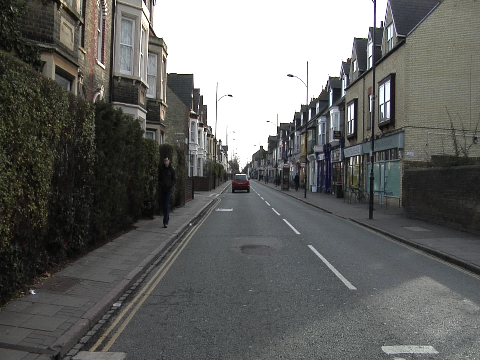
\includegraphics[height=0.125\linewidth]{BayesianSegNet/segnet_bayes_00016_input.png}
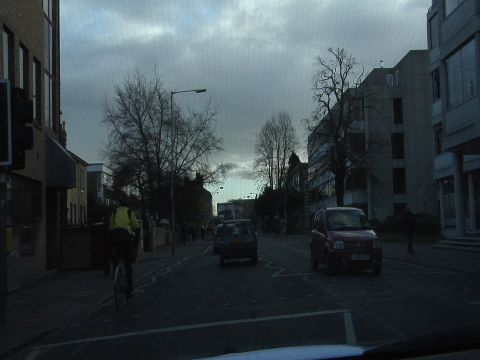
\includegraphics[height=0.125\linewidth]{BayesianSegNet/segnet_bayes_00172_input.png}
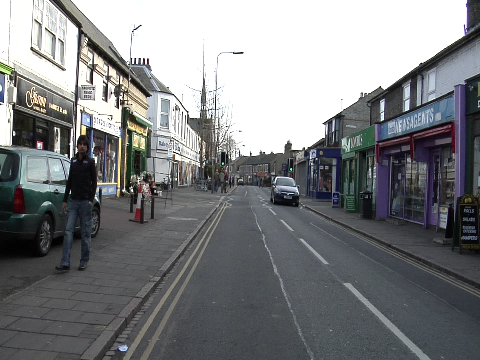
\includegraphics[height=0.125\linewidth]{BayesianSegNet/segnet_bayes_00145_input.png}
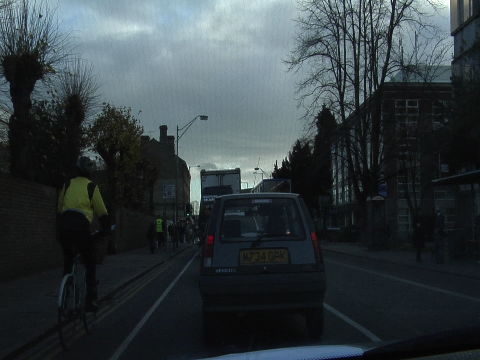
\includegraphics[height=0.125\linewidth]{BayesianSegNet/segnet_bayes_00183_input.png}
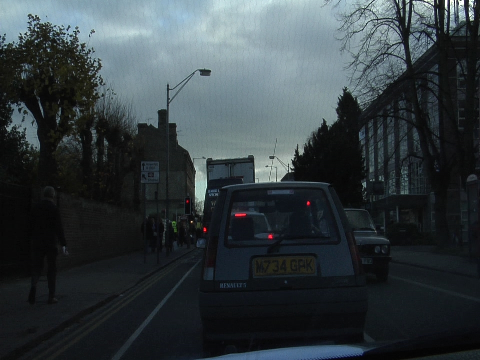
\includegraphics[height=0.125\linewidth]{BayesianSegNet/segnet_bayes_00193_input.png}
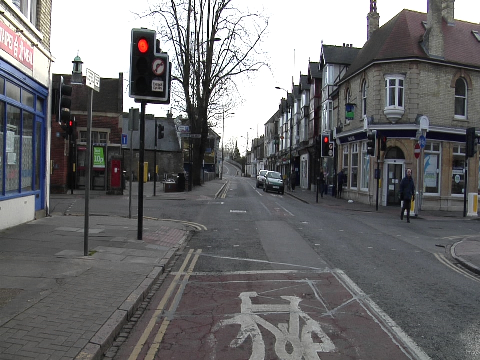
\includegraphics[height=0.125\linewidth]{BayesianSegNet/segnet_bayes_00083_input.png}
}
\resizebox{0.85\linewidth}{!}{
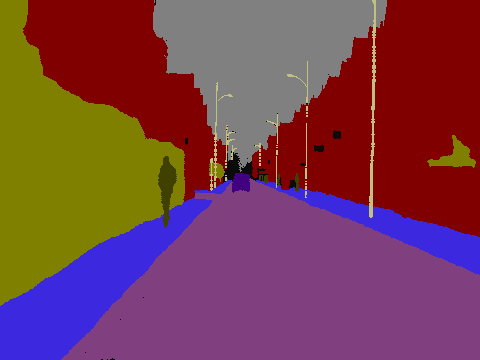
\includegraphics[height=0.125\linewidth]{BayesianSegNet/segnet_bayes_00016_gt.png}
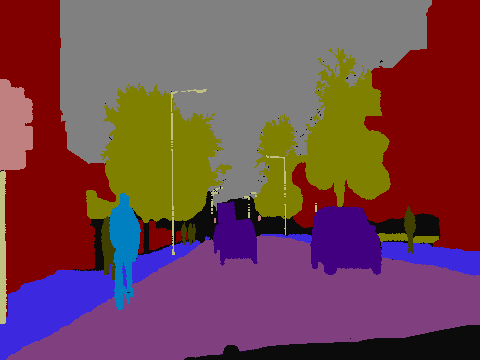
\includegraphics[height=0.125\linewidth]{BayesianSegNet/segnet_bayes_00172_gt.png}
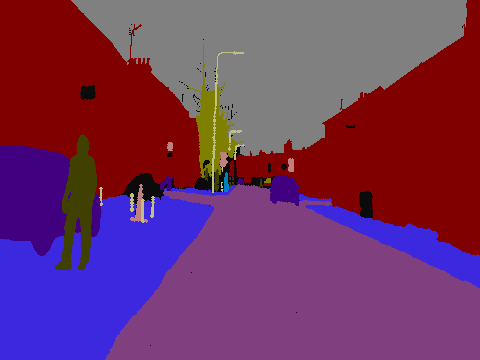
\includegraphics[height=0.125\linewidth]{BayesianSegNet/segnet_bayes_00145_gt.png}
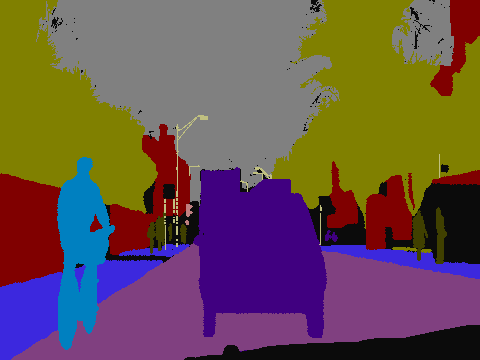
\includegraphics[height=0.125\linewidth]{BayesianSegNet/segnet_bayes_00183_gt.png}
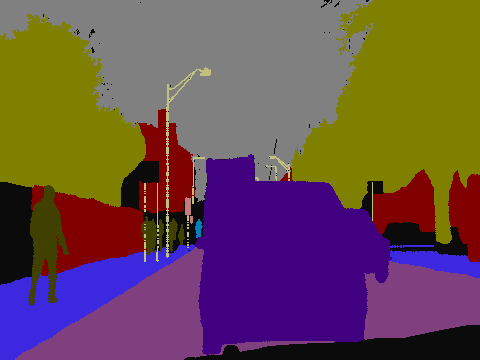
\includegraphics[height=0.125\linewidth]{BayesianSegNet/segnet_bayes_00193_gt.png}
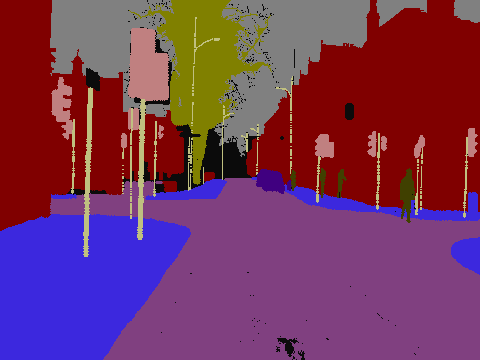
\includegraphics[height=0.125\linewidth]{BayesianSegNet/segnet_bayes_00083_gt.png}
}
\resizebox{0.85\linewidth}{!}{
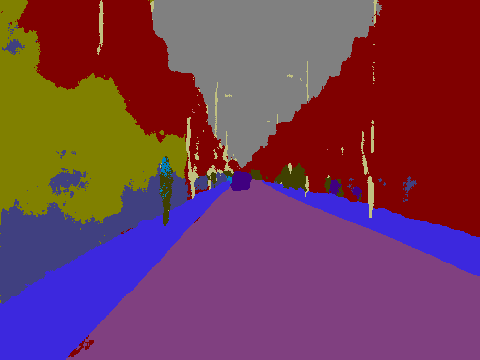
\includegraphics[height=0.125\linewidth]{BayesianSegNet/segnet_bayes_00016_segmentation.png}
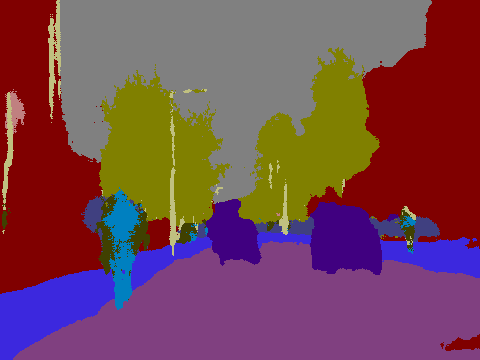
\includegraphics[height=0.125\linewidth]{BayesianSegNet/segnet_bayes_00172_segmentation.png}
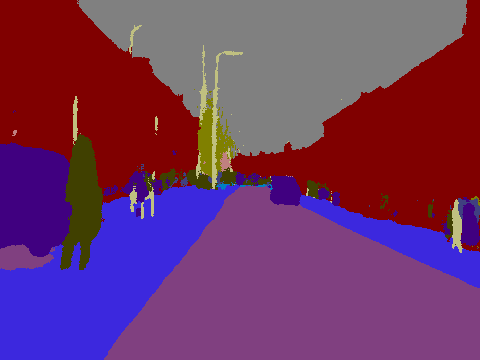
\includegraphics[height=0.125\linewidth]{BayesianSegNet/segnet_bayes_00145_segmentation.png}
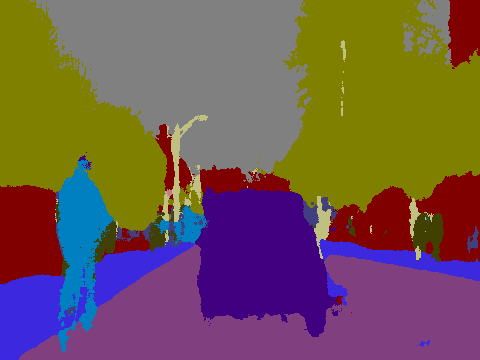
\includegraphics[height=0.125\linewidth]{BayesianSegNet/segnet_bayes_00183_segmentation.png}
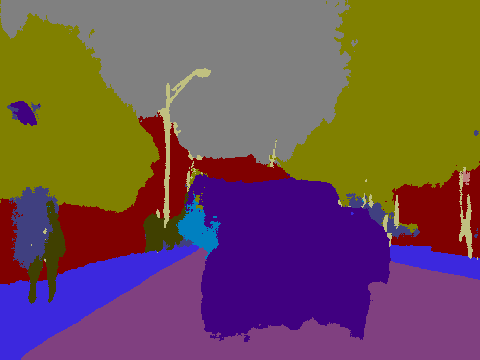
\includegraphics[height=0.125\linewidth]{BayesianSegNet/segnet_bayes_00193_segmentation.png}
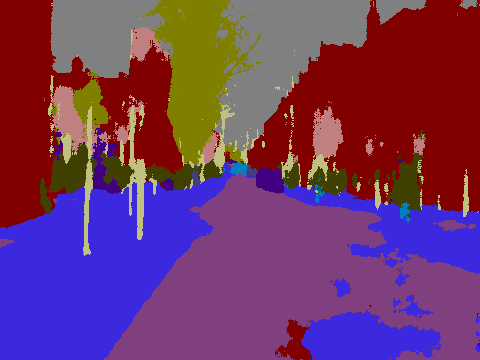
\includegraphics[height=0.125\linewidth]{BayesianSegNet/segnet_bayes_00083_segmentation.png}
}
\resizebox{0.85\linewidth}{!}{
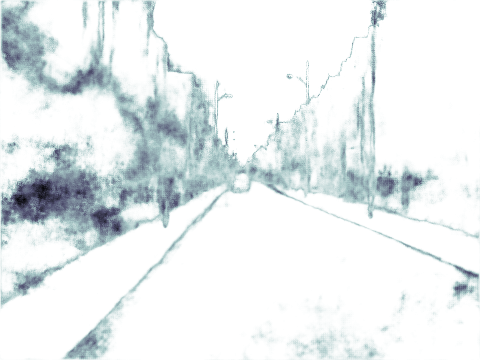
\includegraphics[height=0.125\linewidth]{BayesianSegNet/segnet_bayes_00016_uncertainty.png}
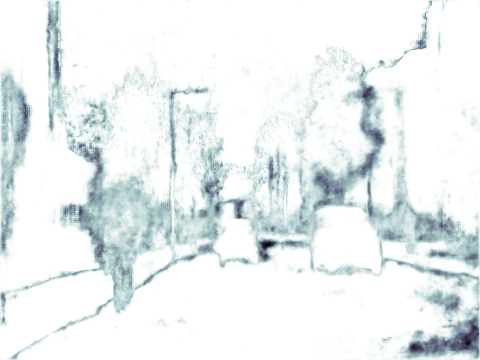
\includegraphics[height=0.125\linewidth]{BayesianSegNet/segnet_bayes_00172_uncertainty.png}
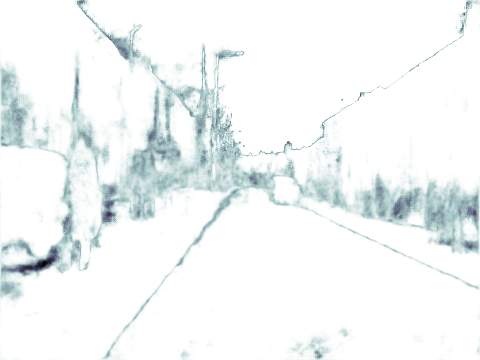
\includegraphics[height=0.125\linewidth]{BayesianSegNet/segnet_bayes_00145_uncertainty.png}
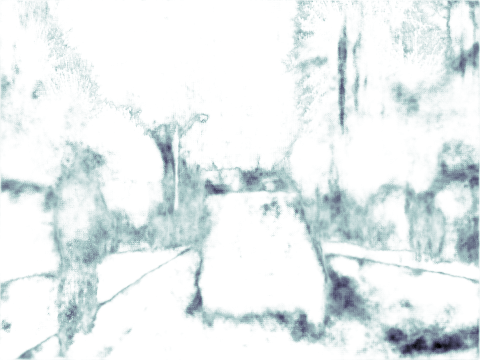
\includegraphics[height=0.125\linewidth]{BayesianSegNet/segnet_bayes_00183_uncertainty.png}
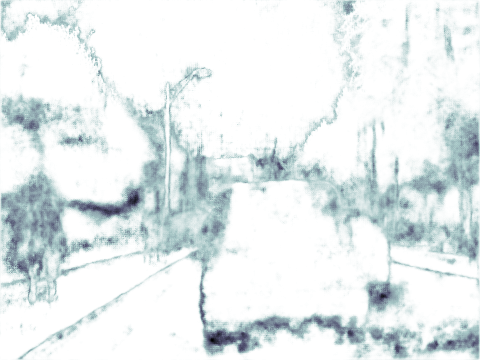
\includegraphics[height=0.125\linewidth]{BayesianSegNet/segnet_bayes_00193_uncertainty.png}
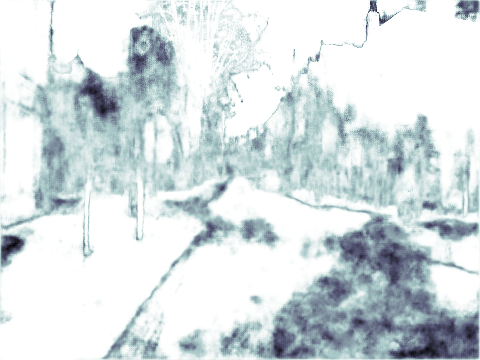
\includegraphics[height=0.125\linewidth]{BayesianSegNet/segnet_bayes_00083_uncertainty.png}
}
\end{center}
   \small{\caption[Bayesian SegNet results on the CamVid dataset.]{\footnotesize\textbf{Bayesian SegNet results on CamVid dataset \citep{brostow2009semantic}.} From top: input image, ground truth, Bayesian SegNet's segmentation prediction, and overall model uncertainty averaged across all classes.
   }}
\label{fig:qual_camvid}

\begin{center}
\resizebox{0.85\linewidth}{!}{
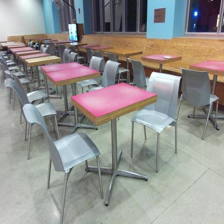
\includegraphics[height=0.125\linewidth]{BayesianSegNet/segnet_bayes_00244_input.png}
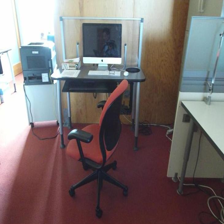
\includegraphics[height=0.125\linewidth]{BayesianSegNet/segnet_bayes_00309_input.png}
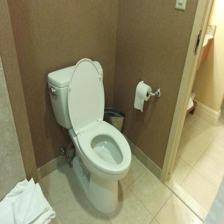
\includegraphics[height=0.125\linewidth]{BayesianSegNet/segnet_bayes_00414_input.png}
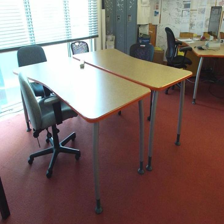
\includegraphics[height=0.125\linewidth]{BayesianSegNet/segnet_bayes_00375_input.png}
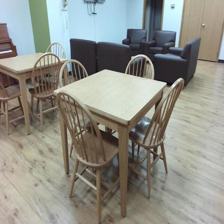
\includegraphics[height=0.125\linewidth]{BayesianSegNet/segnet_bayes_00461_input.png}
\includegraphics[height=0.125\linewidth]{BayesianSegNet/segnet_bayes_00116_input.png}
\includegraphics[height=0.125\linewidth]{BayesianSegNet/segnet_bayes_01035_input.png}
\includegraphics[height=0.125\linewidth]{BayesianSegNet/segnet_bayes_00856_input.png}
}
\resizebox{0.85\linewidth}{!}{
\includegraphics[height=0.125\linewidth]{BayesianSegNet/segnet_bayes_00244_gt.png}
\includegraphics[height=0.125\linewidth]{BayesianSegNet/segnet_bayes_00309_gt.png}
\includegraphics[height=0.125\linewidth]{BayesianSegNet/segnet_bayes_00414_gt.png}
\includegraphics[height=0.125\linewidth]{BayesianSegNet/segnet_bayes_00375_gt.png}
\includegraphics[height=0.125\linewidth]{BayesianSegNet/segnet_bayes_00461_gt.png}
\includegraphics[height=0.125\linewidth]{BayesianSegNet/segnet_bayes_00116_gt.png}
\includegraphics[height=0.125\linewidth]{BayesianSegNet/segnet_bayes_01035_gt.png}
\includegraphics[height=0.125\linewidth]{BayesianSegNet/segnet_bayes_00856_gt.png}
}
\resizebox{0.85\linewidth}{!}{
\includegraphics[height=0.125\linewidth]{BayesianSegNet/segnet_bayes_00244_segmentation.png}
\includegraphics[height=0.125\linewidth]{BayesianSegNet/segnet_bayes_00309_segmentation.png}
\includegraphics[height=0.125\linewidth]{BayesianSegNet/segnet_bayes_00414_segmentation.png}
\includegraphics[height=0.125\linewidth]{BayesianSegNet/segnet_bayes_00375_segmentation.png}
\includegraphics[height=0.125\linewidth]{BayesianSegNet/segnet_bayes_00461_segmentation.png}
\includegraphics[height=0.125\linewidth]{BayesianSegNet/segnet_bayes_00116_segmentation.png}
\includegraphics[height=0.125\linewidth]{BayesianSegNet/segnet_bayes_01035_segmentation.png}
\includegraphics[height=0.125\linewidth]{BayesianSegNet/segnet_bayes_00856_segmentation.png}
}
\resizebox{0.85\linewidth}{!}{
\includegraphics[height=0.125\linewidth]{BayesianSegNet/segnet_bayes_00244_uncertainty.png}
\includegraphics[height=0.125\linewidth]{BayesianSegNet/segnet_bayes_00309_uncertainty.png}
\includegraphics[height=0.125\linewidth]{BayesianSegNet/segnet_bayes_00414_uncertainty.png}
\includegraphics[height=0.125\linewidth]{BayesianSegNet/segnet_bayes_00375_uncertainty.png}
\includegraphics[height=0.125\linewidth]{BayesianSegNet/segnet_bayes_00461_uncertainty.png}
\includegraphics[height=0.125\linewidth]{BayesianSegNet/segnet_bayes_00116_uncertainty.png}
\includegraphics[height=0.125\linewidth]{BayesianSegNet/segnet_bayes_01035_uncertainty.png}
\includegraphics[height=0.125\linewidth]{BayesianSegNet/segnet_bayes_00856_uncertainty.png}
}
\end{center}
\caption[Bayesian SegNet results on the SUN RGB-D dataset.]{\footnotesize \textbf{Bayesian SegNet results on the SUN RGB-D dataset \citep{song2015sun}.}}
\label{fig:qual_sun}

\begin{center}
\resizebox{0.85\linewidth}{!}{
\includegraphics[height=0.125\linewidth]{BayesianSegNet/segnet_bayes_00005_input.png}
\includegraphics[height=0.125\linewidth]{BayesianSegNet/segnet_bayes_00052_input.png}
\includegraphics[height=0.125\linewidth]{BayesianSegNet/segnet_bayes_00202_input.png}
\includegraphics[height=0.125\linewidth]{BayesianSegNet/segnet_bayes_00147_input.png}
\includegraphics[height=0.125\linewidth]{BayesianSegNet/segnet_bayes_00148_input.png}
\includegraphics[height=0.125\linewidth]{BayesianSegNet/segnet_bayes_00166_input.png}
\includegraphics[height=0.125\linewidth]{BayesianSegNet/segnet_bayes_00017_input.png}
\includegraphics[height=0.125\linewidth]{BayesianSegNet/segnet_bayes_00023_input.png}
}
\resizebox{0.85\linewidth}{!}{
\includegraphics[height=0.125\linewidth]{BayesianSegNet/segnet_bayes_00005_segmentation.png}
\includegraphics[height=0.125\linewidth]{BayesianSegNet/segnet_bayes_00052_segmentation.png}
\includegraphics[height=0.125\linewidth]{BayesianSegNet/segnet_bayes_00202_segmentation.png}
\includegraphics[height=0.125\linewidth]{BayesianSegNet/segnet_bayes_00147_segmentation.png}
\includegraphics[height=0.125\linewidth]{BayesianSegNet/segnet_bayes_00148_segmentation.png}
\includegraphics[height=0.125\linewidth]{BayesianSegNet/segnet_bayes_00166_segmentation.png}
\includegraphics[height=0.125\linewidth]{BayesianSegNet/segnet_bayes_00017_segmentation.png}
\includegraphics[height=0.125\linewidth]{BayesianSegNet/segnet_bayes_00023_segmentation.png}
}
\resizebox{0.85\linewidth}{!}{
\includegraphics[height=0.125\linewidth]{BayesianSegNet/segnet_bayes_00005_uncertainty.png}
\includegraphics[height=0.125\linewidth]{BayesianSegNet/segnet_bayes_00052_uncertainty.png}
\includegraphics[height=0.125\linewidth]{BayesianSegNet/segnet_bayes_00202_uncertainty.png}
\includegraphics[height=0.125\linewidth]{BayesianSegNet/segnet_bayes_00147_uncertainty.png}
\includegraphics[height=0.125\linewidth]{BayesianSegNet/segnet_bayes_00148_uncertainty.png}
\includegraphics[height=0.125\linewidth]{BayesianSegNet/segnet_bayes_00166_uncertainty.png}
\includegraphics[height=0.125\linewidth]{BayesianSegNet/segnet_bayes_00017_uncertainty.png}
\includegraphics[height=0.125\linewidth]{BayesianSegNet/segnet_bayes_00023_uncertainty.png}
}
\end{center}
\caption[Bayesian SegNet results on the Pascal VOC dataset.]{\footnotesize \textbf{Pascal VOC 2012 dataset \citep{pascal}.}}
\label{fig:qual_pascal}
\end{figure}
% \begin{figure}[h!]
% \centering
% \resizebox{\linewidth}{!}{
% \includegraphics[width=0.18\linewidth]{segnet_5_output_0.png}
% \includegraphics[width=0.18\linewidth]{segnet_5_output_2.png}
% \includegraphics[width=0.18\linewidth]{segnet_5_output_1.png}
% \includegraphics[width=0.18\linewidth]{segnet_5_output_3.png}
% \includegraphics[width=0.18\linewidth]{segnet_5_output_4.png}}
% \caption[NYUv2 40-Class segmentation.]{NYUv2 40-Class segmentation. From top-left: input image, ground truth, segmentation, aleatoric and epistemic uncertainty.}
% \label{fig:nyu_qual}
% \end{figure}

\begin{figure*}[p]
\centering
\resizebox{\linewidth}{!}{
\includegraphics[width=0.3\linewidth,trim={40 10 40 60},clip]{segnet_55_output_0.png}
\includegraphics[width=0.3\linewidth,trim={40 10 40 60},clip]{segnet_55_output_1.png}
\includegraphics[width=0.3\linewidth,trim={40 10 40 60},clip]{segnet_55_output_2.png}
\includegraphics[width=0.3\linewidth,trim={40 10 40 60},clip]{segnet_55_output_3.png}
\includegraphics[width=0.3\linewidth]{segnet_55_output_4.png}}
~
\resizebox{\linewidth}{!}{
\includegraphics[width=0.3\linewidth,trim={40 10 40 60},clip]{segnet_60_output_0.png}
\includegraphics[width=0.3\linewidth,trim={40 10 40 60},clip]{segnet_60_output_1.png}
\includegraphics[width=0.3\linewidth,trim={40 10 40 60},clip]{segnet_60_output_2.png}
\includegraphics[width=0.3\linewidth,trim={40 10 40 60},clip]{segnet_60_output_3.png}
\includegraphics[width=0.3\linewidth]{segnet_60_output_4.png}}
~
\resizebox{\linewidth}{!}{
\includegraphics[width=0.3\linewidth,trim={40 10 40 60},clip]{segnet_139_output_0.png}
\includegraphics[width=0.3\linewidth,trim={40 10 40 60},clip]{segnet_139_output_1.png}
\includegraphics[width=0.3\linewidth,trim={40 10 40 60},clip]{segnet_139_output_2.png}
\includegraphics[width=0.3\linewidth,trim={40 10 40 60},clip]{segnet_139_output_3.png}
\includegraphics[width=0.3\linewidth]{segnet_139_output_4.png}}
\caption[NYUv2 Depth results.]{NYUv2 Depth results. From left: input image, ground truth, depth regression, aleatoric uncertainty, and epistemic uncertainty.}
\label{fig:nyud_qual}
% \end{figure*}

% \begin{figure*}[h]
\centering
\resizebox{\linewidth}{!}{
\includegraphics[width=0.3\linewidth]{segnet_125_output_0.png}
\includegraphics[width=0.3\linewidth]{segnet_125_output_1.png}
\includegraphics[width=0.3\linewidth]{segnet_125_output_2.png}
\includegraphics[width=0.3\linewidth]{segnet_125_output_3.png}
\includegraphics[width=0.3\linewidth]{segnet_125_output_4.png}}
~
\resizebox{\linewidth}{!}{
\includegraphics[width=0.3\linewidth]{segnet_117_output_0.png}
\includegraphics[width=0.3\linewidth]{segnet_117_output_1.png}
\includegraphics[width=0.3\linewidth]{segnet_117_output_2.png}
\includegraphics[width=0.3\linewidth]{segnet_117_output_3.png}
\includegraphics[width=0.3\linewidth]{segnet_117_output_4.png}}
~
% \resizebox{\linewidth}{!}{
% \includegraphics[width=0.3\linewidth]{segnet_111_output_0.png}
% \includegraphics[width=0.3\linewidth]{segnet_111_output_1.png}
% \includegraphics[width=0.3\linewidth]{segnet_111_output_2.png}
% \includegraphics[width=0.3\linewidth]{segnet_111_output_3.png}
% \includegraphics[width=0.3\linewidth]{segnet_111_output_4.png}}
% ~
\resizebox{\linewidth}{!}{
\includegraphics[width=0.3\linewidth]{segnet_11_output_0.png}
\includegraphics[width=0.3\linewidth]{segnet_11_output_1.png}
\includegraphics[width=0.3\linewidth]{segnet_11_output_2.png}
\includegraphics[width=0.3\linewidth]{segnet_11_output_3.png}
\includegraphics[width=0.3\linewidth]{segnet_11_output_4.png}}
\caption[Qualitative results on the Make3D depth regression dataset.]{Qualitative results on the Make3D depth regression dataset. Left to right: input image, ground truth, depth prediction, aleatoric uncertainty, epistemic uncertainty. 
% Make3D does not provide labels for depth greater than 70m, therefore these distances dominate the epistemic uncertainty signal. Aleatoric uncertainty is prevalent around depth edges or distant points.
}
\label{fig:make3d_qual}
\end{figure*}


\subsubsection{Qualitative observations}
\cref{fig:qual_camvid} shows segmentations and model uncertainty results from Bayesian SegNet (SegNet evaluated with Monte Carlo dropout \citep{kendall2015bayesian}) on CamVid Road Scenes \citep{brostow2009semantic}. \cref{fig:qual_sun} shows SUN RGB-D Indoor Scene Understanding \citep{song2015sun} results and \cref{fig:qual_pascal} has Pascal VOC \citep{pascal} results. These figures show the qualitative performance of Bayesian SegNet. We observe that segmentation predictions are smooth, with a sharp segmentation around object boundaries. Also, when the model predicts an incorrect label, the model uncertainty is generally very high. More generally, we observe that a high model uncertainty is predominantly caused by three situations.

Firstly, at class boundaries the model often displays a high level of uncertainty. This reflects the ambiguity surrounding the definition of defining where these labels transition. The Pascal results clearly illustrated this in \cref{fig:qual_pascal}.

Secondly, objects which are visually difficult to identify often appear uncertain to the model. This is often the case when objects are occluded or at a distance from the camera.

The third situation causing model uncertainty is when the object appears visually ambiguous to the model. As an example, cyclists in the CamVid results (\cref{fig:qual_camvid}) are visually similar to pedestrians, and the model often displays uncertainty around them. We observe similar results with visually similar classes in SUN (\cref{fig:qual_sun}) such as chair and sofa, or bench and table. In Pascal this is often observed between cat and dog, or train and bus classes.

\begin{figure}[t]
    \centering
    \begin{subfigure}[t]{0.45\linewidth}
        \centering
        \includegraphics[width=\linewidth]{scatter_camvid-eps-converted-to.pdf}
        \label{fig:unc_acc2}
        \caption{Performance vs. mean model uncertainty}
    \end{subfigure}
    \begin{subfigure}[t]{0.45\linewidth}
        \centering
        \includegraphics[width=\linewidth]{scatter_camvid_freq-eps-converted-to.pdf}
        \label{fig:unc_freq2}
        \caption{Class frequency vs. mean model uncertainty}
    \end{subfigure}
	\caption[Analysis of Bayesian SegNet's model uncertainty.]{\textbf{Bayesian SegNet performance and frequency compared to mean model uncertainty} for each class in CamVid road scene understanding dataset. These figures show a strong inverse relationships. We observe in (a) that the model is more confident with more accurate classes. (b) shows classes that Bayesian SegNet is more confident at are more prevalent in the dataset. Conversely, for the more rare classes such as Sign Symbol and Bicyclist, Bayesian SegNet has a much higher model uncertainty.}
\end{figure}

\subsubsection{Quality of Uncertainty Metric}

To understand what causes the model to be uncertain, we have plotted the relationship between uncertainty and accuracy in \cref{fig:unc_acc2} and between uncertainty and the frequency of each class in the dataset in \cref{fig:unc_freq2}. Uncertainty is calculated as the mean uncertainty value for each pixel of that class in a test dataset. We observe an inverse relationship between uncertainty and class accuracy or class frequency. This shows that the model is more confident about classes which are easier or occur more often, and less certain about rare and challenging classes.

In \cref{sec:results} we showed that modelling aleatoric and epistemic uncertainty improves prediction performance, with the combination performing even better. In this section we show similar trade-offs for the performance of the uncertainty estimate. We compare aleatoric and epistemic uncertainty quantitatively and again show that aleatoric is more effective in big-data settings, however the combination performs best.

\begin{figure}[h]
    \centering
    \begin{subfigure}[t]{0.45\linewidth}
        \centering
        \includegraphics[width=\linewidth]{class_precision_recall}
        \caption{Classification (CamVid)}
    \end{subfigure}
    ~ 
    \begin{subfigure}[t]{0.45\linewidth}
        \centering
        \includegraphics[width=\linewidth]{regression_precision_recall}
        \caption{Regression (Make3D)}
    \end{subfigure}
    \caption[Precision Recall plots.]{Precision Recall plots demonstrating both measures of uncertainty can effectively capture accuracy for examples similar to the training dataset, as precision decreases with increasing uncertainty.}
\label{fig:prec_recall}
\end{figure}

Firstly, in \cref{fig:prec_recall} we show precision-recall curves for regression and classification models. They show how our model performance improves by removing pixels with uncertainty larger than various percentile thresholds. This illustrates two behaviours of aleatoric and epistemic uncertainty measures. Firstly, it shows that the uncertainty measurements are able to correlate well with accuracy, because all curves are strictly decreasing functions. We observe that precision is lower when we have more points that the model is not certain about. Secondly, the curves for epistemic and aleatoric uncertainty models are very similar. This shows that each uncertainty ranks pixel confidence similarly to the other uncertainty, in the absence of the other uncertainty.
This suggests that when only one uncertainty is explicitly modelled, it attempts to compensate for the lack of the alternative uncertainty when possible.

\begin{figure*}[h]
\centering
    \begin{subfigure}[t]{0.33\linewidth}
        \centering
       \includegraphics[width=\linewidth]{calibration_plots_regression}
        \caption{Regression (Make3D)}
    \end{subfigure}
    \begin{subfigure}[t]{0.3\linewidth}
        \centering
       \includegraphics[width=\linewidth, trim=10mm 0mm 115mm 0mm, clip]{calibration_plots}
        \caption{Classification (CamVid)}
    \end{subfigure}
    \begin{subfigure}[t]{0.32\linewidth}
        \centering
       \includegraphics[width=\linewidth, trim=140mm 15mm 0mm 0mm, clip]{calibration_plots}
%         \caption{Classification (CamVid)}
    \end{subfigure}
\caption[Uncertainty calibration plots.]{Uncertainty calibration plots. This plot shows how well uncertainty is calibrated, where perfect calibration corresponds to the line $y=x$, shown in black. We observe an improvement in calibration mean squared error with aleatoric, epistemic and the combination of uncertainties.}
\label{fig:calibrationplot}
\end{figure*}


Secondly, in \cref{fig:calibrationplot} we analyse the quality of our uncertainty measurement using calibration plots from our model on the test set. To form calibration plots for classification models, we discretize our model’s predicted probabilities into a number of bins, for all classes and all pixels in the test set. We then plot the frequency of correctly predicted labels for each bin of probability values. Better performing uncertainty estimates should correlate more accurately with the line $y=x$ in the calibration plots. For regression models, we can form calibration plots by comparing the frequency of residuals lying within varying thresholds of the predicted distribution. Figure \ref{fig:calibrationplot} shows the calibration of our classification and regression uncertainties.




\begin{table*}[t]
\centering
    \begin{subtable}[t]{\linewidth}
        \centering
          \begin{tabular}{l|l|c|c|c}
    \toprule
          Train & Test & & Aleatoric & Epistemic  \\
          dataset & dataset & RMS & variance & variance  \\ 
          \midrule
          Make3D / 4 & Make3D & 5.76 & 0.506 & 7.73 \\
          Make3D / 2 & Make3D & 4.62 & 0.521 & 4.38 \\
          Make3D & Make3D & 3.87 & 0.485 & 2.78\\
          \midrule
          Make3D / 4 & NYUv2 & - & 0.388 & 15.0 \\
          Make3D & NYUv2 & - & 0.461 & 4.87 \\
    \bottomrule
          \end{tabular}
        \caption{Regression}
    \end{subtable}%
    
    
    \begin{subtable}[t]{\linewidth}
        \centering
          \begin{tabular}{l|l|c|c|c}
    \toprule
          Train & Test & & Aleatoric & Epistemic logit \\
          dataset & dataset & IoU & entropy & variance ($\times10^{-3}$)  \\ 
    \midrule
          CamVid / 4 & CamVid & 57.2 & 0.106 & 1.96 \\
          CamVid / 2 & CamVid & 62.9 & 0.156 & 1.66 \\
          CamVid & CamVid & 67.5 & 0.111 & 1.36 \\
    \midrule
          CamVid / 4 & NYUv2 & - & 0.247 & 10.9 \\
          CamVid & NYUv2 & - & 0.264 & 11.8 \\
    \bottomrule
          \end{tabular}
        \caption{Classification}
    \end{subtable}
\caption[Accuracy of aleatoric and epistemic uncertainties.]{Accuracy of aleatoric and epistemic uncertainties for a range of different train and test dataset combinations. We show aleatoric and epistemic uncertainty as the mean value of all pixels in the test dataset. We compare reduced training set sizes (1, \sfrac{1}{2}, \sfrac{1}{4}) and unrelated test datasets. This shows that aleatoric uncertainty remains approximately constant, while epistemic uncertainty decreases the closer the test data is to the training distribution, demonstrating that epistemic uncertainty can be explained away with sufficient training data (but not for out-of-distribution data).}
\label{datasetsize}
\end{table*}


\subsubsection{Uncertainty with Distance from Training Data}

In this section we show two results:
\begin{enumerate}
\item Aleatoric uncertainty cannot be explained away with more data,
\item Aleatoric uncertainty does not increase for out-of-data examples (situations different from training set), whereas epistemic uncertainty is required to capture uncertainty from situations different from training set.
\end{enumerate}

% Firstly, in 
In Table \ref{datasetsize} we give accuracy and uncertainty for models trained on increasing sized subsets of datasets. This shows that epistemic uncertainty decreases as the training dataset gets larger. It also shows that aleatoric uncertainty remains relatively constant and cannot be explained away with more data.
Testing the models with a different test set (bottom two lines) shows that epistemic uncertainty increases considerably on those test points which lie far from the training sets.
% and the test data is further from each training point (note the two different test sets used for each training set)







% To run this metric:
%CUDA_VISIBLE_DEVICES=0 python experiments/uncertainty/evaluate_uncertainty_regression.py --data-dir /data/cvfs/agk34/Make3D/ --data-type make3d --height 352 --width 448 --data-uncertainty --classification --snapshot /data/cvfs/agk34/experiments/icml/session_2017_02_18_19_38_21_make3d_depth_densenet_448x320_b3_rmsprop_uncertainty/snapshots/snapshot_155000

% Secondly, in Figure \ref{fig:featurevector} we plot the relationship between uncertainty and distance to the training dataset. As a distance measure, we use the dense feature vectors of the BNN before the final logit regression layer, and compute the Euclidean distance to the nearest neighbor in the training dataset. This is done on an image level, taking the mean feature vector over all pixels. We observe that epistemic uncertainty has a slight increasing trend as we get further from the training dataset, while aleatoric uncertainty decreases. 

These results reinforce the case that epistemic uncertainty can be explained away with enough data, but is required to capture situations not encountered in the training set. This is particularly important for safety-critical systems, where epistemic uncertainty is required to detect situations which have never been seen by the model before.



% \begin{figure}[b]
%     \centering
%     \begin{subfigure}[t]{0.5\linewidth}
%         \centering
%         \includegraphics[width=\linewidth]{regression_nearest_neighbour_aleatoric}
%         \caption{Aleatoric}
%     \end{subfigure}%
%     ~ 
%     \begin{subfigure}[t]{0.5\linewidth}
%         \centering
%         \includegraphics[width=\linewidth]{regression_nearest_neighbour_epistemic}
%         \caption{Epistemic}
%     \end{subfigure}
%     \caption{Plot of uncertainty against distance to the nearest training example (in BNN feature space) for the Make3D depth regression test set, with a line of best fit plotted.}
% \label{fig:featurevector}
% \end{figure}



\subsubsection{Real-Time Application}

Our model based on DenseNet \citep{jegou2016one} can process a $640\times480$ resolution image in $150ms$ on a NVIDIA Titan X GPU. The aleatoric uncertainty models add negligible compute. However, epistemic models require expensive Monte Carlo dropout sampling. For models such as ResNet \citep{he2004multiscale}, this is possible to achieve economically because only the last few layers contain dropout. Other models, like DenseNet, require the entire architecture to be sampled. This is difficult to parallelise due to GPU memory constraints, and often results in a $50\times$ slow-down for 50 Monte Carlo samples.

































%%%%%%%%% BODY TEXT
\section{Jointly Learning Geometry and Semantics}
\label{sec:mlttask}

Scene understanding requires knowledge of both geometry and semantics. In this section, we wish to jointly learn both geometry and semantics with a single representation.
This is a form of multi-task learning, which aims to improve learning efficiency and prediction accuracy by learning multiple objectives from a shared representation \citep{caruana1998multitask}. Multi-task learning is prevalent in many applications of machine learning -- from computer vision \citep{kokkinos2016ubernet} to natural language processing \citep{collobert2008unified} to speech recognition \citep{huang2013cross}.

We explore multi-task learning within the setting of visual scene understanding in computer vision. Scene understanding algorithms must understand both the geometry and semantics of the scene at the same time. This forms an interesting multi-task learning problem because scene understanding involves joint learning of various regression and classification tasks with different units and scales. Multi-task learning of visual scene understanding is of crucial importance in systems where long computation run-time is prohibitive, such as the ones used in robotics. Combining all tasks into a single model reduces computation and allows these systems to run in real-time.

Prior approaches to simultaneously learning multiple tasks use a na{\"i}ve weighted sum of losses, where the loss weights are uniform, or manually tuned \citep{sermanet2013overfeat,kokkinos2016ubernet,eigen2015predicting}. However, we show that performance is highly dependant on an appropriate choice of weighting between each task's loss. Searching for an optimal weighting is prohibitively expensive and difficult to resolve with manual tuning. We observe that the optimal weighting of each task is dependant on the measurement scale (e.g. meters, centimetres or millimetres) and ultimately the magnitude of the task's noise. In this work we propose a principled way of combining multiple loss functions to simultaneously learn multiple objectives using homoscedastic uncertainty. We interpret homoscedastic uncertainty as task-dependant weighting and show how to derive a principled multi-task loss function which can learn to balance various regression and classification losses. Our method can learn to balance these weightings optimally, resulting in superior performance, compared with learning each task individually. 

\begin{figure*}[t]
\begin{center}
		\includegraphics[width=\linewidth]{figures/multitask-architecture.pdf}    
\end{center}
   \caption[Multitask deep learning for scene understanding.]{\textbf{Multi-task deep learning.} We derive a principled way of combining multiple regression and classification loss functions for multi-task learning. Our architecture takes a single monocular RGB image as input and produces a pixel-wise classification, an instance semantic segmentation and an estimate of per pixel depth. Multi-task learning can improve accuracy over separately trained models because cues from one task, such as depth, are used to regularize and improve the generalization of another domain, such as segmentation.}
\label{fig:teaser}
\end{figure*}

Specifically, we demonstrate our method in learning scene geometry and semantics with three tasks. Firstly, we learn to classify objects at a pixel level, also known as semantic segmentation \citep{long2015fully,badrinarayanan2017segnet,YuKoltun2016,chen2016deeplab,CRFRNN}. Secondly, our model performs instance segmentation, which is the harder task of segmenting separate masks for each individual object in an image (for example, a separate, precise mask for each individual car on the road) \citep{pinheiro2015learning,hariharan2015hypercolumns,dai2016instance,bai2016deep}. This is a more complicated task than semantic segmentation, as it requires not only an estimate of each pixel's class, but also which object that pixel belongs to. It is also more complicated than object detection, which often predicts object bounding boxes alone \citep{girshick2014rich}. Finally, our model predicts pixel-wise metric depth. Depth by recognition has been demonstrated using dense prediction networks with supervised \citep{eigen2015predicting} and unsupervised \citep{garg2016unsupervised} deep learning. However it is very hard to estimate depth in a way which generalises well. We show that we can improve our estimation of geometry \textit{and} depth by using semantic labels and multi-task deep learning.

In existing literature, separate deep learning models would be used to learn depth regression, semantic segmentation and instance segmentation to create a complete scene understanding system. Given a single monocular input image, our system is the first to produce a semantic segmentation, a dense estimate of metric depth and an instance level segmentation jointly (\fig{teaser}). While other vision models have demonstrated multi-task learning, we show how to learn to combine semantics and geometry. Combining these tasks into a single model ensures that the model agrees between the separate task outputs while reducing computation. Finally, we show that using a shared representation with multi-task learning improves performance on various metrics, making the models more effective.

In summary, the key contributions of this Section are:
\begin{enumerate}
\item a novel and principled multi-task loss to simultaneously learn various classification and regression losses of varying quantities and units using homoscedastic task uncertainty,
\item a unified architecture for semantic segmentation, instance segmentation and depth regression,
\item demonstrating the importance of loss weighting in multi-task deep learning and how to obtain superior performance compared to equivalent separately trained models.
\end{enumerate}

\subsection{Multitask Learning}

We first review related work from the field of multi-task learning. Multi-task learning aims to improve learning efficiency and prediction accuracy for for each task, when compared to training the models separately \citep{thrun1996learning,baxter2000model}. It can be considered an approach to inductive knowledge transfer which improves generalisation by sharing the domain information between complimentary tasks. It does this by using a shared representation to learn multiple tasks -- what is learned from one task can help other tasks be learned better \citep{caruana1998multitask}.

Fine-tuning \citep{agrawal2015learning,oquab2014learning} is a basic example of multi-task learning, where we can leverage different learning tasks by considering them as a pre-training step.
Other models alternate learning between each training task, for example in natural language processing \citep{collobert2008unified}.
Multi-task learning can also be used in a data streaming setting \citep{thrun1996learning}, or to prevent forgetting previously learned tasks in reinforcement learning \citep{kirkpatrick2017overcoming}. It can also be used to learn unsupervised features from various data sources with an auto-encoder \citep{ngiam2011multimodal}.

In computer vision there are many examples of methods for multi-task learning. Many focus on semantic tasks, such as classification and semantic segmentation \citep{liao2016understand} or classification and detection \citep{sermanet2013overfeat}. MultiNet \citep{teichmann2016multinet} proposes an architecture for detection, classification and semantic segmentation. CrossStitch networks \citep{misra2016cross} explore methods to combine multi-task neural activations. Uhrig et al. \citep{uhrig2016pixel} learn semantic and instance segmentations under a classification setting. Multi-task deep learning has also been used for geometry and regression tasks. \citep{eigen2015predicting} show how to learn semantic segmentation, depth and surface normals. PoseNet \citep{kendall2015posenet} is a model which learns camera position and orientation. UberNet \citep{kokkinos2016ubernet} learns a number of different regression and classification tasks under a single architecture. In this work we are the first to propose a method for jointly learning depth regression, semantic and instance segmentation. Like the model of \citep{eigen2015predicting}, our model learns both semantic and geometry representations, which is important for scene understanding. However, our model learns the much harder task of instance segmentation which requires knowledge of both semantics and geometry. This is because our model must determine the class and spatial relationship for each pixel in each object for instance segmentation.

More importantly, all previous methods which learn multiple tasks simultaneously use a na{\"i}ve weighted sum of losses, where the loss weights are uniform, or crudely and manually tuned. In this work we propose a principled way of combining multiple loss functions to simultaneously learn multiple objectives using homoscedastic task uncertainty. We illustrate the importance of appropriately weighting each task in deep learning to achieve good performance and show that our method can learn to balance these weightings optimally.

\begin{figure*}[t]
\centering
\begin{subfigure}[c]{0.5\linewidth}
\resizebox{\linewidth}{!}{
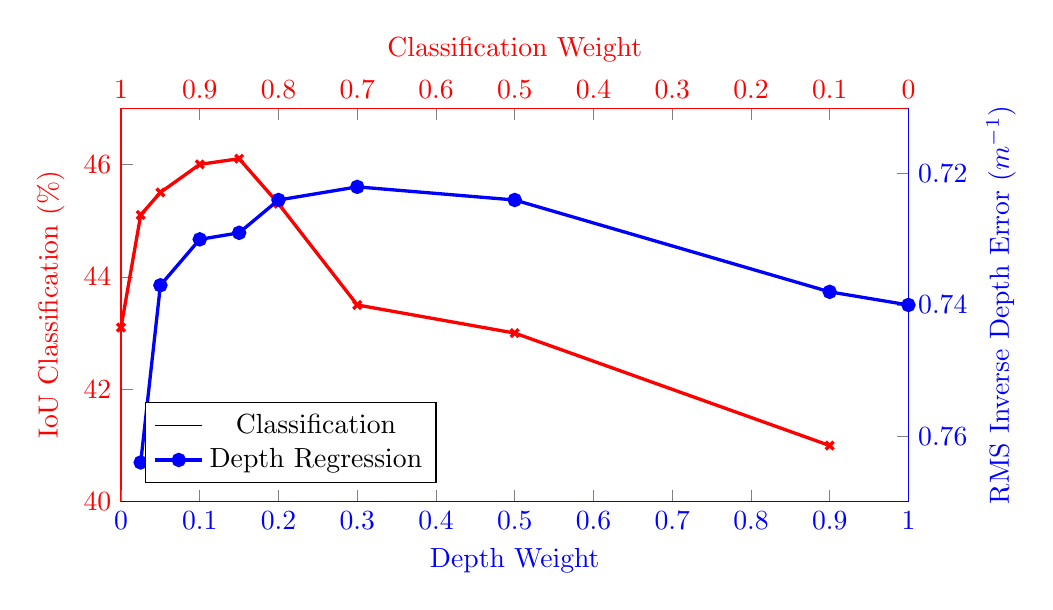
\begin{tikzpicture}
\pgfplotsset{
    compat=1.3,
    scale only axis,
    height=5cm,
    width=10cm, % \textwidth minus width of longest label text minus label offset
    legend style={at={(0.03,0.15)},anchor=west},
}

\pgfplotsset{
  axis line style={red},
  every axis label/.append style ={red},
  every tick label/.append style={red}  
}

\begin{axis}[
  axis y line*=left,
  axis x line*=top,
  ymin=40, ymax=47,
  x dir=reverse,
  xlabel=Classification Weight,
  ylabel=IoU Classification ($\%$),
  xmin=0, xmax=1,
]
\addplot[mark=x,red,very thick]
  coordinates{
    (1.0,43.1)
    (0.975,45.1)
    (0.95,45.5)
    (0.9,46.0)
    (0.85,46.1)
    (0.8,45.3)
    (0.7,43.5)
    (0.5,43.0)
    (0.1,41.0)
}; \label{plot_one2}
\addlegendentry{Classification}
\end{axis}

\pgfplotsset{
  axis line style={blue},
  every axis label/.append style ={blue},
  every tick label/.append style={blue}  
}

\begin{axis}[
  axis y line*=right,
  axis x line*=bottom,
  xlabel=Depth Weight,
  xmin=0, xmax=1,
  ymin=0.71, ymax=0.77,
  ylabel=RMS Inverse Depth Error ($m^{-1}$),
  y dir=reverse,
]
\addlegendimage{/pgfplots/refstyle=plot_one2}\addlegendentry{Classification}
\addplot[mark=*,blue,very thick]
  coordinates{
    (0.025,0.764)
    (0.05,0.737)
    (0.1,0.730)
    (0.15,0.729)
    (0.2,0.724)
    (0.3,0.722)
    (0.5,0.724)
    (0.9,0.738)
    (1.0,0.740)
}; \label{plot_two2}
\addlegendentry{Depth Regression}
\end{axis}
\end{tikzpicture}}
\end{subfigure}
\qquad\qquad
\begin{subfigure}[c]{0.3\linewidth}
\resizebox{\linewidth}{!}{
\begin{tabular}{cc|cc}
    \toprule
\multicolumn{2}{c|}{Task Weights} & Class & Depth \\
Class & Depth & IoU {[}$\%${]} & RMS {[}$m^{-1}${]}\\
    \midrule
1.0 & 0.0 & 43.1 & - \\ %
0.975&0.025& 45.1 & 0.764 \\ % 91k
0.95& 0.05& 45.5 & 0.737 \\ %
0.9 & 0.1 & 46.0 & 0.730 \\ % 63k
0.85& 0.15& 46.1 & 0.729 \\ % 180k
0.8 & 0.2 & 45.3 & 0.724 \\ %
0.7 & 0.3 & 43.5 & 0.722 \\ %
0.5 & 0.5 & 43.0 & 0.724 \\ % 87k
0.1 & 0.9 & 41.0 & 0.738 \\ %
0.0 & 1.0 & - & 0.740 \\ %
    \midrule
\multicolumn{2}{c|}{\textbf{Learned weights}} & \multirow{3}{*}{\textbf{46.2}} & \multirow{3}{*}{\textbf{0.714}} \\
\multicolumn{2}{c|}{\textbf{with task uncertainty}} && \\
\multicolumn{2}{c|}{\textbf{(this work, \sct{mt_loss})}} && \\
    \bottomrule
\end{tabular}}
\end{subfigure}
\vspace{2pt}

(a) Comparing loss weightings when learning \textbf{semantic classification and depth regression}
%%%%%%%%%%%%%%%%%%%%%%%%%%%%%%%%%%%%%%%%%%%%%%%%%%%%%%%%%%%%%
%\noindent\rule{14cm}{0.4pt}

\begin{subfigure}[c]{0.5\linewidth}
\resizebox{\linewidth}{!}{
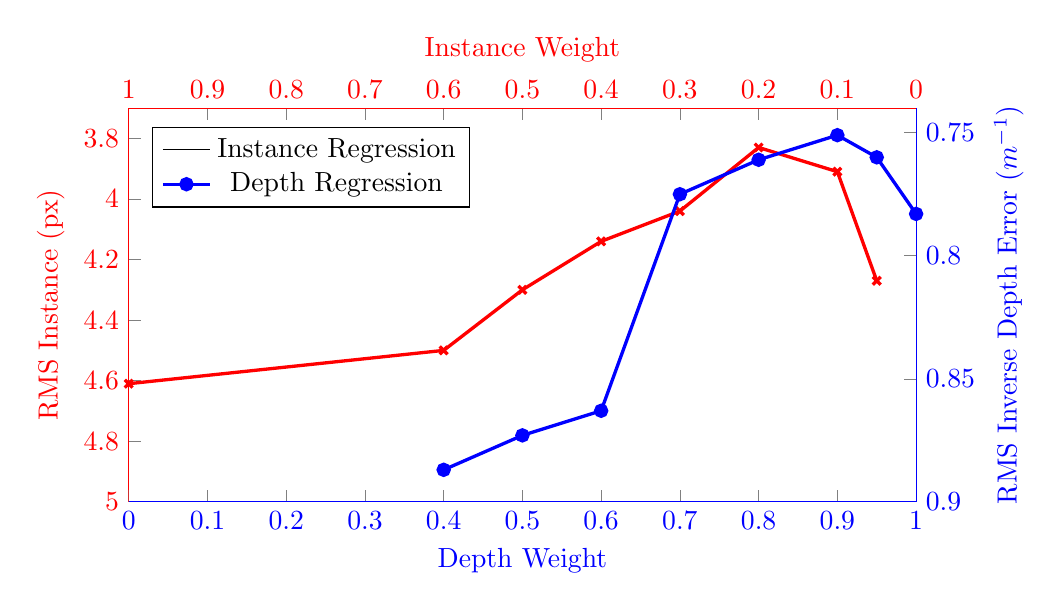
\begin{tikzpicture}
\pgfplotsset{
    compat=1.3,
    scale only axis,
    height=5cm,
    width=10cm, % \textwidth minus width of longest label text minus label offset
    legend style={at={(0.03,0.85)},anchor=west},
}

\pgfplotsset{
  axis line style={red},
  every axis label/.append style ={red},
  every tick label/.append style={red}  
}

\begin{axis}[
  axis y line*=left,
  axis x line*=top,
  ymin=3.7, ymax=5.0,
  x dir=reverse,
  xlabel=Instance Weight,
  ylabel=RMS Instance (px),
  xmin=0, xmax=1,
  y dir=reverse,
]
\addplot[mark=x,red,very thick]
  coordinates{
    (1.0,4.61)
    (0.6,4.50)
    (0.5,4.30)
    (0.4,4.14)
    (0.3,4.04)
    (0.2,3.83)
    (0.1,3.91)
    (0.05,4.27)
}; \label{plot_one}
\addlegendentry{Instance Regression}
\end{axis}

\pgfplotsset{
  axis line style={blue},
  every axis label/.append style ={blue},
  every tick label/.append style={blue}  
}

\begin{axis}[
  axis y line*=right,
  axis x line*=bottom,
  xlabel=Depth Weight,
  xmin=0, xmax=1,
  ymin=0.74, ymax=0.9,
  ylabel=RMS Inverse Depth Error ($m^{-1}$),
  y dir=reverse,
]
\addlegendimage{/pgfplots/refstyle=plot_one}\addlegendentry{Instance Regression}
\addplot[mark=*,blue,very thick]
  coordinates{
    (0.4,0.887)
    (0.5,0.873)
    (0.6,0.863)
    (0.7,0.775)
    (0.8,0.761)
    (0.9,0.751)
    (0.95,0.760)
    (1.0,0.783)
}; \label{plot_two}
\addlegendentry{Depth Regression}
\end{axis}
\end{tikzpicture}}
\end{subfigure}
\qquad\qquad
\begin{subfigure}[c]{0.3\linewidth}
\resizebox{\linewidth}{!}{
\begin{tabular}{cc|cc}
    \toprule
\multicolumn{2}{c|}{Task Weights} & Instance & Depth \\
Instance & Depth & RMS {[}px{]} & RMS {[}$m^{-1}${]}\\ 
    \midrule
1.0 & 0.0 & 4.61 & - \\ %
0.6 & 0.4 & 4.50 & 0.887 \\
0.5 & 0.5 & 4.30 & 0.873 \\
0.4 & 0.6 & 4.14 & 0.863 \\
0.3 & 0.7 & 4.04 & 0.775 \\
0.2 & 0.8 & 3.83 & 0.761 \\
0.1 & 0.9 & 3.91 & 0.751 \\
0.05 & 0.95 & 4.27 & 0.760 \\
0.0 & 1.0 & - & 0.783 \\ %
    \midrule
\multicolumn{2}{c|}{\textbf{Learned weights}} & \multirow{3}{*}{\textbf{4.06}} & \multirow{3}{*}{\textbf{0.744}} \\
\multicolumn{2}{c|}{\textbf{with task uncertainty}} && \\
\multicolumn{2}{c|}{\textbf{(this work, \sct{mt_loss})}} && \\
    \bottomrule
\end{tabular}}
\end{subfigure}
%%%%%%%%%%%%%%%%%%%%%%%%%%%%%%%%%%%%%%%%%%%%%%%%%%%%%%%%%%%%%

(b) Comparing loss weightings when learning \textbf{instance regression and depth regression}
%\noindent\rule{14cm}{0.4pt}

   \caption[Effect of varying task weights for multitask learning.]{\textbf{Learning multiple tasks improves the model's representation and individual task performance}. These figures and tables illustrate the advantages of multi-task learning for (a) semantic classification and depth regression and (b) instance and depth regression. Performance of the model in individual tasks is seen at both edges of the plot where $w=0$ and $w=1$. For some balance of weightings between each task, we observe improved performance for both tasks. All models were trained with a learning rate of $0.01$ with the respective weightings applied to the losses using the loss function in \eqn{basic_loss}. Results are shown using the Tiny CityScapes validation dataset using a down-sampled resolution of $128\times256$.}
\label{fig:scale_factor}
\end{figure*}

\subsection{Multi Task Learning with Homoscedastic Uncertainty}
\label{sec:multitask}

Multi-task learning concerns the problem of optimising a model with respect to multiple objectives. It is prevalent in many deep learning problems. The naive approach to combining multi objective losses would be to simply perform a weighted linear sum of the losses for each individual task:
\begin{equation}
\label{eqn:basic_loss}
L_{total}= \sum_i w_i L_{i}.
\end{equation}
This is the dominant approach used by prior work \citep{teichmann2016multinet,sermanet2013overfeat,liao2016understand,uhrig2016pixel}, for example for dense prediction tasks \citep{kokkinos2016ubernet}, for scene understanding tasks \citep{eigen2015predicting} and for rotation (in quaternions) and translation (in meters) for camera pose \citep{kendall2015posenet}. However, there are a number of issues with this method. Namely, model performance is extremely sensitive to weight selection, $w_i$, as illustrated in \fig{scale_factor}. These weight hyper-parameters are expensive to tune, often taking many days for each trial. Therefore, it is desirable to find a more convenient approach which is able to learn the optimal weights.

More concretely, let us consider a network which learns to predict pixel-wise depth and semantic class from an input image. In \fig{scale_factor} the two boundaries of each plot show models trained on individual tasks, with the curves showing performance for varying weights $w_i$ for each task. We observe that at some optimal weighting, the joint network performs better than separate networks trained on each task individually (performance of the model in individual tasks is seen at both edges of the plot: $w=0$ and $w=1$). At near-by values to the optimal weight the network performs worse on one of the tasks. However, searching for these optimal weightings is expensive and increasingly difficult with large models with numerous tasks. We next show how to learn optimal task weightings using ideas from probabilistic modelling. Additionally, we show a similar result for two regression tasks; instance segmentation and depth regression.

\subsection{Homoscedastic uncertainty as task-dependant uncertainty}
\label{sec:uncertainty}

In \cref{seg_unc}, we explained that there are two main types of uncertainty one can model \citep{kendall2017uncertainties}.
\begin{itemize}
\item \textit{Epistemic uncertainty} is uncertainty in the model, which captures what our model doesn’t know due to lack of training data. It can be explained away with increased training data.
\item \textit{Aleatoric uncertainty} captures our uncertainty with respect to information which our data cannot explain. Aleatoric uncertainty can be explained away with the ability to observe all explanatory variables with increasing precision.
\end{itemize}
However, we now go one step further than \cref{seg_unc}. Aleatoric uncertainty can again be divided into two sub-categories.
\begin{itemize}
\item \textit{Data-dependant} or \textit{Heteroscedastic} uncertainty is aleatoric uncertainty which depends on the input data and is predicted as a model output.
\item \textit{Task-dependant} or \textit{Homoscedastic} uncertainty is  aleatoric uncertainty which is not dependant on the input data. It is not a model output, rather it is a quantity which stays constant for all input data and varies between different tasks. It can therefore be described as task-dependant uncertainty.
\end{itemize}
In a multi-task setting, we show that the task uncertainty captures the relative confidence between tasks, reflecting the uncertainty inherent to the regression or classification task. It will also depend on the task's representation or unit of measure.  We propose that we can use homoscedastic uncertainty as a basis for weighting losses in a multi-task learning problem.

\subsection{Multi-task likelihoods}
\label{sec:mt_loss}

In this section we derive a multi-task loss function based on maximising the Gaussian likelihood with homoscedastic uncertainty.
Let $\f^\W(\x)$ be the output of a neural network with weights $\W$ on input $\x$. We define the following probabilistic model. 
For regression tasks we define our likelihood as a Gaussian with mean given by the model output:
\begin{equation}
p(\y | \f^\W(\x)) = \N(\f^\W(\x), \sigma^2)
\end{equation}
with an observation noise scalar $\sigma$. 
For classification we often squash the model output through a softmax function, and sample from the resulting probability vector:
% \newcommand{\softmax}{\text{softmax}}
\begin{equation}
p(\y | \f^\W(\x)) = \softmax(\f^\W(\x)).
\end{equation}

In the case of multiple model outputs, we often define the likelihood to factorise over the outputs, given some sufficient statistics. We define $\f^\W(\x)$ as our sufficient statistics, and obtain the following multi-task likelihood:
\begin{equation}
p(\y_1, ..., \y_K | \f^\W(\x)) = p(\y_1 | \f^\W(\x)) ... p(\y_K | \f^\W(\x))
\end{equation}
with model outputs $\y_1, ..., \y_K$ (such as semantic segmentation, depth regression, etc).

In \textit{maximum likelihood} inference, we maximise the log likelihood of the model.
In regression, for example, the log likelihood can be written as
\begin{equation}
\log p(\y | \f^{\W}(\x)) \propto 
-\frac{1}{2 \sigma^2}||\y - \f^{\W}(\x)||^2 - \log \sigma
\end{equation}
for a Gaussian likelihood (or similarly for a Laplace likelihood)
with $\sigma$ the model's observation noise parameter -- capturing how much noise we have in the outputs. We then maximise the log likelihood with respect to the model parameters $\W$ and observation noise parameter $\sigma$.

Let us now assume that our model output is composed of two vectors $\y_1$ and $\y_2$, each following a Gaussian distribution:
\begin{equation}
\begin{split}
p(\y_1, \y_2 | \f^\W(\x)) &= 
p(\y_1 | \f^\W(\x)) \cdot p(\y_2 | \f^\W(\x)) \\
&= 
\N(\y_1; \f^\W(\x), \sigma_1^2) \cdot
\N(\y_2; \f^\W(\x), \sigma_2^2).
\end{split}
\end{equation}

This leads to the \textit{minimisation} objective, $\cL(\W, \sigma_1, \sigma_2)$, (our loss) for our multi-output model:
\begin{equation}
\begin{split}
\cL(\W, \sigma_1, \sigma_2) &= 
- \log p(\y_1, \y_2 | \f^\W(\x)) \\
&\propto
\frac{1}{2 \sigma_1^2} ||\y_1 - \f^{\W}(\x)||^2
+ \frac{1}{2 \sigma_2^2} ||\y_2 - \f^{\W}(\x)||^2 
+ \log \sigma_1 \sigma_2 \\
&= \frac{1}{2 \sigma_1^2} \cL_1(\W) 
+ \frac{1}{2 \sigma_2^2} \cL_2(\W)
+ \log \sigma_1 \sigma_2
\end{split}
\end{equation}
Where we wrote $\cL_1(\W) = ||\y_1 - \f^{\W}(\x)||^2$ for the loss of the first output variable, and similarly for $\cL_2(\W)$.

% Rewriting this objective 

We interpret minimising this last objective with respect to $\sigma_1$ and $\sigma_2$ as learning the relative weight of the losses $\cL_1(\W)$ and $\cL_2(\W)$ adaptively, based on the data. As $\sigma_1$ -- the noise parameter for the variable $\y_1$ -- increases, we have that the weight of $\cL_1(\W)$ decreases. On the other hand, as the noise decreases, we have that the weight of the respective objective increases. The noise is discouraged from increasing too much (effectively ignoring the data) by the last term in the objective, which acts as a regulariser for the noise terms.

This construction can be trivially extended to multiple regression outputs. However, the extension to classification likelihoods is more interesting. We adapt the classification likelihood to squash a \textit{scaled} version of the model output through a softmax function:
\begin{equation}
p(\y | \f^\W(\x), \sigma) = \softmax( \frac{1}{\sigma^2} \f^\W(\x))
\end{equation}
with a positive scalar $\sigma$. The log likelihood for this output can then be written as 
\begin{equation}
\log p(\y = c | \f^\W(\x), \sigma) = \frac{1}{\sigma^2} f^\W_c(\x) - \log \sum_{c'} \exp \bigg( \frac{1}{\sigma^2} f^\W_{c'}(\x) \bigg)
\end{equation}
with $f^\W_c(\x)$ the $c$'th element of the vector $\f^\W(\x)$.

Next, assume that a model's multiple outputs are composed of a continuous output $\y_1$ and a discrete output $\y_2$, modelled with a Gaussian likelihood and a softmax likelihood, respectively. Like before, the joint loss is given as:
\begin{equation}
\begin{aligned}
\cL(\W, \sigma_1, \sigma_2) &= 
-\log p(\y_1, \y_2=c | \f^\W(\x)) \\
&= 
-\log \N(\y_1; \f^\W(\x), \sigma_1^2) \cdot
\softmax(\y_2=c; \f^\W(\x), \sigma_2) \\
&=
\frac{1}{2 \sigma_1^2} ||\y_1 - \f^{\W}(\x)||^2
+ \log \sigma_1
- \log p(\y_2 = c | \f^\W(\x), \sigma_2)
 \\
&= \frac{1}{2 \sigma_1^2} \cL_1(\W) 
+ \frac{1}{\sigma_2^2} \cL_2(\W)
+ \log \sigma_1 
+ \log \frac{
\sum_{c'} \exp \bigg( \frac{1}{\sigma_2^2} f^\W_{c'}(\x) \bigg)
}{
\bigg( \sum_{c'} \exp \bigg( f^\W_{c'}(\x) \bigg) \bigg)^{\frac{1}{\sigma_2^2} }
}
\\
&\approx \frac{1}{2 \sigma_1^2} \cL_1(\W) 
+ \frac{1}{\sigma_2^2} \cL_2(\W)
+ \log \sigma_1
+ \log \sigma_2,
\end{aligned}
\end{equation}
where again we write $\cL_1(\W) = ||\y_1 - \f^{\W}(\x)||^2$ for the Euclidean loss of $\y_1$, write $\cL_2(\W) = -\log \softmax (\y_2, \f^\W(\x))$ for the cross entropy loss of $\y_2$ (with $\f^{\W}(\x)$ not scaled), and optimise with respect to $\W$ as well as $\sigma_1$, $\sigma_2$.
In the last transition we introduced the explicit simplifying assumption $\frac{1}{\sigma_2^2} \sum_{c'} \exp \bigg( \frac{1}{\sigma_2^2} f^\W_{c'}(\x) \bigg) \approx \bigg( \sum_{c'} \exp \bigg( f^\W_{c'}(\x) \bigg) \bigg)^{\frac{1}{\sigma_2^2} }$ which becomes an equality when $\sigma_2^2 \rightarrow 1$. This has the advantage of simplifying the optimisation objective, as well as empirically improving results.

This last objective can be seen as learning the relative weights of the losses for each output. Large scale values $\sigma_2$ will decrease the contribution of $\cL_2(\W)$, whereas small scale $\sigma_2$ will increase its contribution. The scale is regulated by the last term in the equation. The objective is penalised when setting $\sigma_2$ too large (with the last term contributing a constant value $\log C$ -- with $C$ classes -- to the loss). 

The multi-task objective with homoscedastic task uncertainty now becomes:
\begin{equation}
\cL(\W, \sigma_1, \sigma_2, ..., \sigma_i) = \sum_i \frac{1}{2 \sigma_i^2} \cL_i(\W) + \log \sigma_i
\label{eqn:loss_ch2}
\end{equation}
over all tasks indexed by $i$. Again, we write $\cL_i(\W) = ||\y_i - \f^{\W}(\x)||^2$ for regression losses $\y_i$, and $\cL_i(\W) = -\log \softmax (\y_i, \f^\W(\x))$ for classification losses. This construction can be trivially extended to arbitrary combinations of discrete and continuous variables, allowing us to learn the relative weights of each loss in a principled and well-founded way. This loss is smoothly differentiable, and is well formed such that the task weights will not converge to zero. In contrast, directly learning the weights using a simple linear sum of losses \eqn{basic_loss} would result in weights which quickly converge to zero. In the following sections we introduce our experimental model and present empirical results.

%%%%%%%%%%%%%%%%%%%%%%%%%%%%%%%%%%%%%%%%%%%%%%%%%%%%%%%%%%%%%%%%%%%%%%%%%%%%%%%%%%%%%%%%%%%%%%

\subsection{Scene Understanding Model}

\begin{figure*}[t]
\resizebox{\linewidth}{!}{
\begin{subfigure}[t]{0.24\linewidth}
\begin{center}
		\includegraphics[width=\linewidth,trim={0px 60px 0 0px},clip]{results/segnet_107_output_0.jpg}
		\includegraphics[width=\linewidth,trim={0px 60px 0 0px},clip]{results/segnet_186_output_0.jpg}
		\includegraphics[width=\linewidth,trim={0px 60px 0 0px},clip]{results/segnet_242_output_0.jpg}
		\includegraphics[width=\linewidth,trim={0px 60px 0 0px},clip]{results/segnet_209_output_0.jpg}
  \caption{Input image}
\end{center}
\end{subfigure}
\begin{subfigure}[t]{0.24\linewidth}
\begin{center}
		\includegraphics[width=\linewidth,trim={0px 60px 0 0px},clip]{results/segnet_107_output_1.png}
		\includegraphics[width=\linewidth,trim={0px 60px 0 0px},clip]{results/segnet_186_output_1.png}
		\includegraphics[width=\linewidth,trim={0px 60px 0 0px},clip]{results/segnet_242_output_1.png}
		\includegraphics[width=\linewidth,trim={0px 60px 0 0px},clip]{results/segnet_209_output_1.png}
  \caption{Segmentation output}
\end{center}
\end{subfigure}
\begin{subfigure}[t]{0.24\linewidth}
\begin{center}
		\includegraphics[width=\linewidth,trim={0px 60px 0 0px},clip]{results/segnet_107_output_3.png}
		\includegraphics[width=\linewidth,trim={0px 60px 0 0px},clip]{results/segnet_186_output_3.png}
		\includegraphics[width=\linewidth,trim={0px 60px 0 0px},clip]{results/segnet_242_output_3.png}
		\includegraphics[width=\linewidth,trim={0px 60px 0 0px},clip]{results/segnet_209_output_3.png}
  \caption{Instance output}
\end{center}
\end{subfigure}
\begin{subfigure}[t]{0.24\linewidth}
\begin{center}
		\includegraphics[width=\linewidth,trim={0px 60px 0 0px},clip]{results/segnet_107_output_4.png}
		\includegraphics[width=\linewidth,trim={0px 60px 0 0px},clip]{results/segnet_186_output_4.png}
		\includegraphics[width=\linewidth,trim={0px 60px 0 0px},clip]{results/segnet_242_output_4.png}
		\includegraphics[width=\linewidth,trim={0px 60px 0 0px},clip]{results/segnet_209_output_4.png}
  \caption{Depth output}
\end{center}
\end{subfigure}}
	\caption[Qualitative results on the CityScapes dataset.]{\textbf{Qualitative results for multi-task learning of geometry and semantics for road scene understanding}. Results are shown on test images from the CityScapes dataset using our multi-task approach with a single network trained on all tasks. We observe that multi-task learning improves the smoothness and accuracy for depth perception because it learns a representation that uses cues from other tasks, such as segmentation (and vice versa).}
	\label{fig:cityscapesqual}
\end{figure*}

To understand semantics and geometry we first propose an architecture which can learn regression and classification outputs, at a pixel level. Our architecture is a deep convolutional encoder decoder network \citep{badrinarayanan2017segnet}. Our model consists of a number of convolutional encoders which produce a shared representation, followed by a corresponding number of task-specific convolutional decoders. A high level summary is shown in \fig{teaser}.

The purpose of the encoder is to learn a deep mapping to produce rich, contextual features, using domain knowledge from a number of related tasks. Our encoder is based on ResNet-101 \citep{he2016deep} (without the final fully connected layer). We apply this encoder in a convolutional manner over the input image, which results in a $2048$ dimensional shared feature representation. Inspired by the dilated convolutional approach of \citep{chen2016deeplab}, this encoder feature map is sub-sampled by a factor of 8 compared to the input image dimensions.

We then split the network into separate decoders (with separate weights) for each task. The purpose of the decoder is to learn a mapping from the shared features to an output. Each decoder consists of three convolutional layers with kernel size $3\times3$, $1\times1$ and $1\times1$ respectively, and feature size $512$, $512$ and the number of output dimensions respectively.

\textbf{Semantic Segmentation.}
We use the cross-entropy loss to learn pixel-wise class probabilities, averaging the loss over the pixels with semantic labels in each mini-batch.

\textbf{Instance Segmentation.}
An intuitive method for defining which instance a pixel belongs to is an association to the instance's centroid.
We use a regression approach for instance segmentation \citep{liang2015proposal}. This approach is inspired by \citep{leibe2008robust} which identifies instances using Hough votes from object parts. In this work we extend this idea by using votes from individual pixels using deep learning. We learn an instance vector, $\hat{x}_n$, for each pixel coordinate, $c_n$, which points to the centroid of the pixel's instance, $i_n$, such that $i_n=\hat{x}_n+c_n$. We train this regression with an $L_1$ loss using ground truth labels $x_n$, averaged over all labelled pixels, $N_I$, in a mini-batch: $\cL_{Instance} = \frac{1}{|N_I|} \sum_{N_I} \norm{x_n - \hat{x}_n}_1$.

\fig{instance} details the representation we use for instance segmentation. \fig{instance}(a) shows the input image and a mask of the pixels which are of an instance class (at test time inferred from the predicted semantic segmentation). \fig{instance}(b) and \fig{instance}(c) show the ground truth and predicted instance vectors for both $x$ and $y$ coordinates. We then cluster these votes using OPTICS \citep{ankerst1999optics}, resulting in the predicted instance segmentation output in \fig{instance}(d).

\begin{figure}[t]
\begin{center}
\begin{subfigure}[t]{0.24\linewidth}
  \includegraphics[width=\linewidth]{figures/input.png}
  \includegraphics[width=\linewidth]{figures/mask.png}
  \caption{Input Image\\and Mask}
\end{subfigure}
\begin{subfigure}[t]{0.24\linewidth}
  \includegraphics[width=\linewidth]{figures/gt_x.png}
  \includegraphics[width=\linewidth]{figures/gt_y.png}
  \caption{Instance\\Labels}
\end{subfigure}
\begin{subfigure}[t]{0.24\linewidth}
  \includegraphics[width=\linewidth]{figures/instance_x.png}
  \includegraphics[width=\linewidth]{figures/instance_y.png}
  \caption{Model\\Prediction}
\end{subfigure}
\begin{subfigure}[t]{0.24\linewidth}
  \includegraphics[width=\linewidth]{figures/segmentation.png}
  \includegraphics[width=\linewidth]{figures/instance_segmentation.png}
  \caption{Segmentation Output}
\end{subfigure}
\end{center}
   \caption[Instance centroid regression example.]{\textbf{Instance centroid regression training data.} For each pixel, we regress a vector pointing to the instance's centroid. The loss is computed with the mask, and $x$ and $y$ instance vectors.}
\label{fig:instance}
\end{figure}

One of the most difficult cases for instance segmentation algorithms to handle is when the instance mask is split due to occlusion. \fig{instancemask} shows that our method can handle these situations, by allowing pixels to vote for their instance centroid with geometry. Methods which rely on watershed approaches \citep{bai2016deep}, or instance edge identification approaches fail in these scenarios.

To obtain segmentations for each instance, we now need to estimate the instance centres, $\hat{i}_n$. We propose to consider the estimated instance vectors, $\hat{x}_n$, as votes in a Hough parameter space and use a clustering algorithm to identify these instance centres. OPTICS \citep{ankerst1999optics}, is an efficient density based clustering algorithm. It is able to identify an unknown number of multi-scale clusters with varying density from a given set of samples. We chose OPICS for two reasons. Crucially, it does not assume knowledge of the number of clusters like algorithms such as k-means \citep{macqueen1967some}. Secondly, it does not assume a canonical instance size or density like discretised binning approaches \citep{comaniciu2002mean}. Using OPTICS, we cluster the points $c_n+\hat{x}_n$ into a number of estimated instances, $\hat{i}$. We can then assign each pixel, $p_n$ to the instance closest to its estimated instance vector, $c_n+\hat{x}_n$.

\textbf{Depth Regression.}
We train with supervised labels using pixel-wise metric inverse depth using a $L_1$ loss function: $\cL_{Depth} = \frac{1}{|N_D|} \sum_{N_D} \norm{d_n-\hat{d_n}}_1$. Our architecture estimates inverse depth, $\hat{d}_n$, because it can represent points at infinite distance (such as sky). We can obtain inverse depth labels, $d_n$, from a RGBD sensor or stereo imagery. Pixels which do not have an inverse depth label are ignored in the loss.

\begin{figure}[t]
\begin{center}
\begin{subfigure}[t]{0.49\linewidth}
  \includegraphics[width=\linewidth,trim={350px 120px 0 100px},clip]{results/segnet_19_output_0.jpg}
  \caption{Input Image}
\end{subfigure}
\begin{subfigure}[t]{0.49\linewidth}
  \includegraphics[width=\linewidth,trim={350px 120px 0 100px},clip]{results/segnet_19_output_3.png}
  \caption{Instance Segmentation}
\end{subfigure}
\end{center}
   \caption[Instance segmentation with occlusion.]{This example shows two cars which are occluded by trees and lampposts, making the instance segmentation challenging. Our instance segmentation method can handle occlusions effectively. We can correctly handle segmentation masks which are split by occlusion, yet part of the same instance, By incorporating semantics and geometry.}
\label{fig:instancemask}
\end{figure}

\begin{table*}[t]
\centering
\resizebox{\textwidth}{!}{
\begin{tabular}{l|ccc|c|c|c}
    \toprule
& \multicolumn{3}{c|}{Task Weights} & Classification & Instance & Inverse Depth \\
Loss & Cls. & Inst. & Depth & IoU {[}$\%${]} & RMS Error {[}$px${]} & RMS Error {[}$px${]}\\ 
    \midrule
Class only & 1 & 0 & 0 & 43.1\% &-&-\\
Instance only & 0 & 1 & 0 &-& 4.61 &-\\
Depth only & 0 & 0 & 1 &-&-& 0.783 \\ 
    \midrule
Unweighted sum of losses & 0.333 & 0.333 & 0.333 & 43.6\% & 3.92 & 0.786 \\
% Unweighted sum of losses & 1.0 & 1.0 & 1.0 & 43.0\% & 4.04 & 0.768 \\
    \midrule
Approx. optimal weights & 0.8 & 0.05 & 0.15 & 46.3\% & 3.92 & 0.799 \\
    \midrule
2 task uncertainty weighting & \checkmark & \checkmark & & 46.5\% & 3.73 & - \\%done
2 task uncertainty weighting & \checkmark & & \checkmark & 46.2\% & - & 0.714 \\%done
2 task uncertainty weighting & & \checkmark & \checkmark & - & 4.06 & 0.744 \\%underway
    \midrule
3 task uncertainty weighting & \checkmark & \checkmark & \checkmark & \textbf{46.6\%} & \textbf{3.91} & \textbf{0.702} \\ %underway
    \bottomrule
\end{tabular}}
\caption[Quantitative improvement from multitask learning for scene understanding.]{Quantitative improvement when learning semantic segmentation, instance segmentation and depth with our multi-task loss. Experiments were conducted on the Tiny CityScapes dataset, sub-sampled to a resolution of $128\times 256$, results are shown from the validation set. We observe an improvement in performance when training with our multi-task loss, over both single-task models and weighted losses. Additionally, we observe an improvement when training on all three tasks ($3\times \checkmark$) using our multi-task loss, compared with all pairs of tasks alone (denoted by $2\times \checkmark$). This shows that our loss function can automatically learn an better performing weighting between the tasks.}
\label{tbl:multitasks}
\end{table*}


\afterpage{%
    \clearpage% Flush earlier floats (otherwise order might not be correct)
    \begin{landscape}% Landscape page
\begin{table}[t]
	\centering
	\resizebox{\linewidth}{!}{
		\begin{tabular}{l|c|c|c|c|c|c|c|c|c|c}
        \toprule
			& \multicolumn{4}{c|}{Semantic Segmentation} & \multicolumn{4}{c|}{Instance Segmentation} & \multicolumn{2}{c}{Monocular Disparity Estimation} \\
			Method & IoU class & iIoU class & IoU cat & iIoU cat & AP & AP 50\% & AP 100m & AP 50m & Mean Error {[}$px${]} & RMS Error {[}$px${]} \\ \toprule % & Runtime [s]\\ \hline \hline
			\multicolumn{11}{c}{\textbf{Classification, instance and depth methods (this work)}}\\ \midrule
			Multi-Task Learning & 78.5 & 57.4 & 89.9 & 77.7 & 17.7 & 32.3 & 22.4 & 33.7 & 5.55 & 10.36 \\ \midrule%& - \\
			\multicolumn{11}{c}{\textbf{Classification and instance methods}}\\ \midrule
			Uhrig et al. \citep{uhrig2016pixel} & 64.3 & 41.6 & 85.9 & 73.9 & 8.9 & 21.1 & 15.3 & 16.7 &-&-\\ \midrule%& - \\ \hline
			\multicolumn{11}{c}{\textbf{Instance only methods}}\\ \midrule
			Mask R-CNN \citep{he2017maskrcnn} &-&-&-&-& 26.2 & 49.9 & 37.6 & 40.1 & -& -\\ %& 60.0 \\ \hline
            Deep Watershed \citep{bai2016deep} &-&-&-&-& 19.4 & 35.3 & 31.4 & 36.8 & -& -\\ %& 60.0 \\ \hline
            R-CNN + MCG \citep{Cordts2016Cityscapes} &-&-&-&-& 4.6 & 12.9 & 7.7 & 10.3 & -& -\\ \midrule %& 60.0 \\ \hline
			\multicolumn{11}{c}{\textbf{Classification only methods}}\\ \midrule
			chen2016deeplab V3 \citep{chen2017rethinking} & 81.3 & 60.9 & 91.6 & 81.7 &-&-&-&-&-&-\\%& 
			PSPNet \citep{zhao2017pspnet} & 81.2 & 59.6 & 91.2 & 79.2 &-&-&-&-&-&-\\%& 
			%LRR-4x \citep{ghiasi2016laplacian} & 71.8 & 47.9 & 88.4 & 73.9 &-&-&-&-&-&-\\%& 
			Adelaide \citep{lin2015efficient} & 71.6 & 51.7 & 87.3 & 74.1 &-&-&-&-&-&-\\%& 4.0\\
			chen2016deeplab \citep{chen2016deeplab} & 70.4 & 42.6 & 86.4 & 67.7 &-&-&-&-&-&-\\%& 4.0\\
			Dilation \citep{YuKoltun2016} & 67.1 & 42.0 & 86.5 & 71.1 &-&-&-&-&-&-\\%& 4.0 \\
			FCN 8s \citep{long2015fully} & 65.3 & 41.7 & 85.7 & 70.1 &-&-&-&-&-&-\\%& 0.5 \\
			SegNet \citep{badrinarayanan2017segnet} & 57.0 & 32.0 & 79.1 & 61.9 &-&-&-&-&-&-\\%& 0.06 \\
            \bottomrule
		\end{tabular}}
	\caption[Quantitative results of our multitask scene understanding model.]{\textbf{CityScapes Benchmark \citep{Cordts2016Cityscapes}.} We show results from the validation dataset using the full resolution of $1024\times2048$ For the full leaderboard, please see \url{www.cityscapes-dataset.com/benchmarks}. The disparity (inverse depth) metrics were computed against the CityScapes depth maps, which are sparse and computed using SGM stereo \citep{hirschmuller2005accurate}. Note, these comparisons are not entirely fair, as many methods use ensembles of different training datasets.}
	\label{tbl:benchmarks}
\end{table}
\end{landscape}}


\subsection{Model Evaluation}
\label{sec:tasks}

We demonstrate the efficacy of our method on CityScapes \citep{Cordts2016Cityscapes}, a large dataset for road scene understanding. It comprises of stereo imagery, from automotive grade stereo cameras with a $22cm$ baseline, labelled with instance and semantic segmentations from 20 classes. Depth images are also provided, labelled using SGM \citep{Hirschmuller2008}, which we treat as ground truth to train our monocular depth regression algorithm. Additionally, we assign zero inverse depth to pixels labelled as sky. The dataset was collected from a number of cities in fine weather and consists of 3,250 training and 750 validation images at $2048\times1024$ resolution. 1,000 images are used for testing on an online evaluation server. 

In \tbl{multitasks} we compare individual models to multi-task learning models using a na{\"i}ve weighted loss or the task uncertainty weighting we propose in this Section. To reduce the computational burden, we train each model at a reduced resolution of $128\times256$ pixels. This clearly illustrates the benefit of multi-task learning, which obtains significantly better performing results than individual task models. For example, using our method we improve classification results from $43.1\%$ to $46.6\%$.

We also compare to a number of na{\"i}ve multi-task losses. We compare weighting each task equally and using approximately optimal weights. Using a uniform weighting results in poor performance, in some cases not even improving on the results from the single task model. Obtaining approximately optimal weights is difficult with increasing number of tasks as it requires an expensive grid search over parameters. However, even these weights perform worse compared with our proposed method. \fig{scale_factor} shows that using task uncertainty weights can even perform better compared to optimal weights found through fine-grained grid search. We believe that this is due to two reasons. First, grid search is restricted in accuracy by the resolution of the search. Second, optimising the task weights using a homoscedastic noise term allows for the weights to be dynamic during training. In general, we observe that the uncertainty term decreases during training which improves the optimisation process. 


\begin{figure*}[p]
\makebox[\textwidth][c]{
\resizebox{\linewidth}{!}{
\begin{subfigure}[t]{0.24\linewidth}
\begin{center}
		\includegraphics[width=\linewidth,trim={0px 60px 0 0px},clip]{results/segnet_18_output_0.jpg}
		\includegraphics[width=\linewidth,trim={0px 60px 0 0px},clip]{results/segnet_20_output_0.jpg}
		\includegraphics[width=\linewidth,trim={0px 60px 0 0px},clip]{results/segnet_43_output_0.jpg}
		\includegraphics[width=\linewidth,trim={0px 60px 0 0px},clip]{results/segnet_204_output_0.jpg}
		\includegraphics[width=\linewidth,trim={0px 60px 0 0px},clip]{results/segnet_149_output_0.jpg}
		\includegraphics[width=\linewidth,trim={0px 60px 0 0px},clip]{results/segnet_128_output_0.jpg}
		\includegraphics[width=\linewidth,trim={0px 60px 0 0px},clip]{results/segnet_114_output_0.jpg}
		\includegraphics[width=\linewidth,trim={0px 60px 0 0px},clip]{results/segnet_86_output_0.jpg}
		\includegraphics[width=\linewidth,trim={0px 60px 0 0px},clip]{results/segnet_51_output_0.jpg}
		\includegraphics[width=\linewidth,trim={0px 60px 0 0px},clip]{results/segnet_45_output_0.jpg}
		\includegraphics[width=\linewidth,trim={0px 60px 0 0px},clip]{results/segnet_19_output_0.jpg}
  \caption{Input image}
\end{center}
\end{subfigure}
\begin{subfigure}[t]{0.24\linewidth}
\begin{center}
		\includegraphics[width=\linewidth,trim={0px 60px 0 0px},clip]{results/segnet_18_output_1.png}
		\includegraphics[width=\linewidth,trim={0px 60px 0 0px},clip]{results/segnet_20_output_1.png}
		\includegraphics[width=\linewidth,trim={0px 60px 0 0px},clip]{results/segnet_43_output_1.png}
		\includegraphics[width=\linewidth,trim={0px 60px 0 0px},clip]{results/segnet_204_output_1.png}
		\includegraphics[width=\linewidth,trim={0px 60px 0 0px},clip]{results/segnet_149_output_1.png}
		\includegraphics[width=\linewidth,trim={0px 60px 0 0px},clip]{results/segnet_128_output_1.png}
		\includegraphics[width=\linewidth,trim={0px 60px 0 0px},clip]{results/segnet_114_output_1.png}
		\includegraphics[width=\linewidth,trim={0px 60px 0 0px},clip]{results/segnet_86_output_1.png}
		\includegraphics[width=\linewidth,trim={0px 60px 0 0px},clip]{results/segnet_51_output_1.png}
		\includegraphics[width=\linewidth,trim={0px 60px 0 0px},clip]{results/segnet_45_output_1.png}
		\includegraphics[width=\linewidth,trim={0px 60px 0 0px},clip]{results/segnet_19_output_1.png}
  \caption{Segmentation output}
\end{center}
\end{subfigure}
\begin{subfigure}[t]{0.24\linewidth}
\begin{center}
		\includegraphics[width=\linewidth,trim={0px 60px 0 0px},clip]{results/segnet_18_output_3.png}
		\includegraphics[width=\linewidth,trim={0px 60px 0 0px},clip]{results/segnet_20_output_3.png}
		\includegraphics[width=\linewidth,trim={0px 60px 0 0px},clip]{results/segnet_43_output_3.png}
		\includegraphics[width=\linewidth,trim={0px 60px 0 0px},clip]{results/segnet_204_output_3.png}
		\includegraphics[width=\linewidth,trim={0px 60px 0 0px},clip]{results/segnet_149_output_3.png}
		\includegraphics[width=\linewidth,trim={0px 60px 0 0px},clip]{results/segnet_128_output_3.png}
		\includegraphics[width=\linewidth,trim={0px 60px 0 0px},clip]{results/segnet_114_output_3.png}
		\includegraphics[width=\linewidth,trim={0px 60px 0 0px},clip]{results/segnet_86_output_3.png}
		\includegraphics[width=\linewidth,trim={0px 60px 0 0px},clip]{results/segnet_51_output_3.png}
		\includegraphics[width=\linewidth,trim={0px 60px 0 0px},clip]{results/segnet_45_output_3.png}
		\includegraphics[width=\linewidth,trim={0px 60px 0 0px},clip]{results/segnet_19_output_3.png}
  \caption{Instance output}
\end{center}
\end{subfigure}
\begin{subfigure}[t]{0.24\linewidth}
\begin{center}
		\includegraphics[width=\linewidth,trim={0px 60px 0 0px},clip]{results/segnet_18_output_4.png}
		\includegraphics[width=\linewidth,trim={0px 60px 0 0px},clip]{results/segnet_20_output_4.png}
		\includegraphics[width=\linewidth,trim={0px 60px 0 0px},clip]{results/segnet_43_output_4.png}
		\includegraphics[width=\linewidth,trim={0px 60px 0 0px},clip]{results/segnet_204_output_4.png}
		\includegraphics[width=\linewidth,trim={0px 60px 0 0px},clip]{results/segnet_149_output_4.png}
		\includegraphics[width=\linewidth,trim={0px 60px 0 0px},clip]{results/segnet_128_output_4.png}
		\includegraphics[width=\linewidth,trim={0px 60px 0 0px},clip]{results/segnet_114_output_4.png}
		\includegraphics[width=\linewidth,trim={0px 60px 0 0px},clip]{results/segnet_86_output_4.png}
		\includegraphics[width=\linewidth,trim={0px 60px 0 0px},clip]{results/segnet_51_output_4.png}
		\includegraphics[width=\linewidth,trim={0px 60px 0 0px},clip]{results/segnet_45_output_4.png}
		\includegraphics[width=\linewidth,trim={0px 60px 0 0px},clip]{results/segnet_19_output_4.png}
  \caption{Depth output}
\end{center}
\end{subfigure}}}
	\caption[Further qualitative results on the CityScapes dataset.]{\textbf{More qualitative results of our scene understanding model on test images from the CityScapes dataset.}}
	\label{fig:cityscapesquallarge}
\end{figure*}

\begin{figure}[p]
\begin{subfigure}[t]{\linewidth}
\begin{center}
  \includegraphics[width=0.32\linewidth]{plots/class_loss.eps}
  \includegraphics[width=0.32\linewidth]{plots/class_weight.eps}
  \includegraphics[width=0.32\linewidth]{plots/class_weight_zoom.eps}
  \caption{Semantic classification task}
\end{center}
\end{subfigure}
\begin{subfigure}[t]{\linewidth}
\begin{center}
  \includegraphics[width=0.32\linewidth]{plots/instance_loss.eps}
  \includegraphics[width=0.32\linewidth]{plots/instance_weight.eps}
  \includegraphics[width=0.32\linewidth]{plots/instance_weight_zoom.eps}
  \caption{Instance regression task}
\end{center}
\end{subfigure}
\begin{subfigure}[t]{\linewidth}
\begin{center}
  \includegraphics[width=0.32\linewidth]{plots/depth_loss.eps}
  \includegraphics[width=0.32\linewidth]{plots/depth_weight.eps}
  \includegraphics[width=0.32\linewidth]{plots/depth_weight_zoom.eps}
  \caption{Depth regression task}
\end{center}
\end{subfigure}
   \caption[Convergence of task weights during training.]{\textbf{Training plots showing convergence of homoscedastic noise and task loss} for an array of initialisation choices for the homoscedastic uncertainty terms for all three tasks. The left plot shows that the loss converges to the same minimum from varying initialisation choices. The centre plot shows the the homoscedastic noise value optimises to the same solution from a variety of initialisations. The plots on the right show a zoomed in view of the homoscedastic noise plot, showing the initialisation and convergence over a few hundred training iterations. Despite the network taking $10,000+$ iterations for the training loss to converge, the task uncertainty converges very rapidly after only $~100$ iterations.}
\label{fig:convergence}
\end{figure}


\subsection{Benchmarking}

In \cref{tbl:benchmarks} we benchmark our approach on the full-size $1024 \times 2048$ pixel CityScapes dataset \citep{Cordts2016Cityscapes}. This is a challenging benchmark and we compare to various other state-of-the-art methods for semantic segmentation, instance segmentation and depth prediction. Our approach is the first to perform all three tasks jointly. Although we do not outperform the best semantic segmentation methods, a lot of the techniques proposed by these algorithms are complimentary to ours.

\subsection{Analysis}

This loss is also robust to the value we use to initialise the weights.
One of the attractive properties of our approach to weighting multi-task losses is that it is robust to the initialisation choice for the homoscedastic noise parameters. \fig{convergence} shows that for an array of initial choices of $\log \sigma^2$ from $-2.0$ to $5.0$ the homoscedastic noise and task loss is able to converge to the same minima. Additionally, the homoscedastic noise terms converges after only $~100$ iterations, while the network requires $30,000+$ iterations to train. Therefore our model is robust to the choice of initial value for the weighting terms.
Interestingly, we observe that this loss allows the network to dynamically tune the weighting. Typically, the homoscedastic noise terms decrease in magnitude as training progresses.


An interesting question left unanswered is where the optimal location is for splitting the shared encoder network into separate decoders for each task? And, what network depth is best for the shared multi-task representation?

\section{Summary}

In this chapter, we investigated the problem of scene understanding and estimating the semantics and geometry of a scene from a single image. We briefly summarise the main conclusions within the three main themes of this dissertation.

\textbf{End-to-end deep learning.}
First, we presented SegNet, a deep convolutional network architecture for per-pixel output, capable of being trained end-to-end. The main motivation behind SegNet was the need to design an efficient architecture for road scene understanding which is efficient both in terms of memory and computational time. We analysed SegNet and compared it with other important variants to reveal the trade-offs involved in designing architectures for segmentation. Those which store the encoder network feature maps in full perform best but consume more memory during inference time. SegNet on the other hand is more efficient since it only stores the max-pooling indices of the feature maps and uses them in its decoder network to achieve good performance.

\textbf{Uncertainty.}
We presented a novel Bayesian deep learning framework to learn a mapping to aleatoric uncertainty from the input data, which is composed on top of epistemic uncertainty models based on Monte Carlo dropout. We derived a framework for both regression and classification applications. We showed that it is important to model \textit{aleatoric} uncertainty for:
\begin{itemize}
\item Large data situations, where epistemic uncertainty is explained away,
\item Real-time applications, because we can form aleatoric models without expensive Monte Carlo samples.
\end{itemize}
And \textit{epistemic} uncertainty is important for:
\begin{itemize}
\item Safety-critical applications, because epistemic uncertainty is required to understand examples which are different from training data,
\item Small datasets where the training data is sparse.
\end{itemize}

However aleatoric and epistemic uncertainty models are not mutually exclusive. We showed that the combination is able to achieve new state-of-the-art results on depth regression and semantic segmentation benchmarks.

\textbf{Geometry.}
Finally, in order to construct a scene understanding system, algorithms must learn both semantics and geometry. We showed how to formulate this as a multi-task learning problem. We construct a single model which is capable of learning a single representation of semantics and geometry. 

We showed that correctly weighting loss terms is of paramount importance for multi-task learning problems. We demonstrated that homoscedastic (task) uncertainty is an effective way to weight losses. We derived a principled loss function which can learn a relative weighting automatically from the data and is robust to the weight initialization. We showed that this can improve performance for scene understanding tasks with a unified architecture for semantic segmentation, instance segmentation and per-pixel depth regression. We demonstrated modelling task-dependant homoscedastic uncertainty improves the model's representation and each task's performance when compared to separate models trained on each task individually.
